%%%%%%%%%%%%%%%%%%%%%%% file template.tex %%%%%%%%%%%%%%%%%%%%%%%%%
%
% This is a general template file for the LaTeX package SVJour3
% for Springer journals.          Springer Heidelberg 2010/09/16
%
% Copy it to a new file with a new name and use it as the basis
% for your article. Delete % signs as needed.
%
% This template includes a few options for different layouts and
% content for various journals. Please consult a previous issue of
% your journal as needed.
%
%%%%%%%%%%%%%%%%%%%%%%%%%%%%%%%%%%%%%%%%%%%%%%%%%%%%%%%%%%%%%%%%%%%
%
% First comes an example EPS file -- just ignore it and
% proceed on the \documentclass line
% your LaTeX will extract the file if required
\begin{filecontents*}{example.eps}
%!PS-Adobe-3.0 EPSF-3.0
%%BoundingBox: 19 19 221 221
%%CreationDate: Mon Sep 29 1997
%%Creator: programmed by hand (JK)
%%EndComments
gsave
newpath
  20 20 moveto
  20 220 lineto
  220 220 lineto
  220 20 lineto
closepath
2 setlinewidth
gsave
  .4 setgray fill
grestore
stroke
grestore
\end{filecontents*}
%
\RequirePackage{fix-cm}
%
%\documentclass{svjour3}                     % onecolumn (standard format)
%\documentclass[smallcondensed]{svjour3}     % onecolumn (ditto)
\documentclass[smallextended]{svjour3}       % onecolumn (second format)
%\documentclass[twocolumn]{svjour3}          % twocolumn
%
\smartqed  % flush right qed marks, e.g. at end of proof
%
%设置图片浮动位置的宏包
\usepackage{subfigure} %插入多图时用子图显示的宏包
\usepackage[normalem]{ulem}
\usepackage{bbm}
\useunder{\uline}{\ul}{}
\usepackage{graphicx}
\usepackage{algorithmic}
\usepackage{algorithm}
\usepackage{amsmath,amsfonts,amssymb,amsbsy,bm,paralist,theorem,ifthen,color}
\usepackage{xcolor}
\usepackage{multirow}
\usepackage[numbers]{natbib}
\usepackage[misc]{ifsym}
\usepackage{footmisc} 
%设置图片浮动位置的宏包
\usepackage{subfigure} %插入多图时用子图显示的宏包
\usepackage[normalem]{ulem}
\useunder{\uline}{\ul}{}
%
% \usepackage{mathptmx}      % use Times fonts if available on your TeX system
%
% insert here the call for the packages your document requires
%\usepackage{latexsym}
% etc.
%
% please place your own definitions here and don't use \def but
% \newcommand{}{}
%
% Insert the name of "your journal" with
% \journalname{myjournal}
%
\begin{document}

\title{Dual Self-supervised Variational Autoencoder for Collaborative Filtering}

%\title{Self-supervised Variational Autoencoder for Recommender Systems\IEEEauthorrefmark{1}\\
%\thanks{$^*$ This work was supported in part by the National Natural Science Foundation of China (U1934220) and the Fundamental Research Funds for the Central Universities (GrantNo. 2019JBM316).}}


%\thanks{Grants or other notes
%about the article that should go on the front page should be
%placed here. General acknowledgments should be placed at the end of the article.}

%\subtitle{Do you have a subtitle?\\ If so, write it here}

%\titlerunning{Short form of title}        % if too long for running head


%\author{Jing Wang, Jun Wu, Caiyan Jia, Zhifei Zhang \\ \\(\Letter)\\ %etc.}
%\author{Xinyuan Liu\footnote{\label{note1}Indicates equal contribution.}, Lijuan Sun\footref{note1}\\ Songhe Feng(\Letter) \\  %etc.
%}
%\authorrunning{X. Liu, L. Sun, et al.}
%\authorrunning{J. Wang, et al.}

%\authorrunning{Short form of author list} % if too long for running head



\author{Jing Wang, Jun Wu(\Letter)\\
	Caiyan Jia, Zhifei Zhang\\
	\\ %etc.
}
%\author{Xinyuan Liu\footnote{\label{note1}Indicates equal contribution.}, Lijuan Sun\footref{note1}\\ Songhe Feng(\Letter) \\  %etc.
%}
%\authorrunning{X. Liu, L. Sun, et al.}
\authorrunning{J. Wang, et al.}


\institute{Jing Wang, Jun Wu, Caiyan Jia, Zhifei Zhang  \at
	School of Computer and Information Technology, Beijing Jiaotong University, Beijing, China\\
	\email{\{19125244, cyjia, zhfzhang, wuj\}@bjtu.edu.cn}
}




\date{Received: date / Accepted: date}
% The correct dates will be entered by the editor


\maketitle

\begin{abstract}
Variational autoencoder (VAE) is considered as an emerging model for ensuring competitive performance in recommender systems. However, existing VAE models may fail to provide satisfactory recommendation results in presence of highly sparse user-item interactions. 
%However, its performance is severely limited by the amount of training examples and, as a result, existing 
In this paper, we propose a Dual Self-supervised Variational Autoencoder (DSVAE) model to improve both the generalization ability of VAE model on the sparse interaction datasets and personalized characteristic of recommendation results. Specifically, we supplement the classical supervised  task of  recommendation with dual self-supervised tasks which contains two SSL tasks. One is to align the representations learned from different views, where views are generated by data augmentation, and the other is to discriminate reconstructed feedback data from the rest of user input feedback data. Furthermore, we aim to optimize a combined objective of recommendation task and pretext task, making them to reinforce each other during the learning process. Extensive experiment results on three real-world benchmarks validate the superiority of our DSVAE model to state-of-the-art VAE style recommendation techniques.
\keywords{ Recommender Systems \and Self-supervised Learning\and Variational Autoencoder }
% \PACS{PACS code1 \and PACS code2 \and more}
% \subclass{MSC code1 \and MSC code2 \and more}
\end{abstract}

\section{Introduction}
\label{sec1}
Nowadays, recommender systems have been an indispensable tool in various online applications, including E-commerce platforms, video recommendation, for different users in the situations of information overload. The core recommendation method in RSs is collaborative filtering (CF)
\cite{DBLP:journals/tweb/CachedaCFF11}, which analyzes the users and interdependencies among items, with the goal of identifying unobserved user-item associations. 
%CF is extensively investigated by the current literatures \cite{DBLP:books/sp/Aggarwal16}.
%In the context of collaborative filtering, latent factor model and matrix factorization model are predominant \cite{DBLP:conf/uai/GopalanHB15, DBLP:conf/icdm/HuKV08, DBLP:journals/computer/KorenBV09, DBLP:conf/nips/SalakhutdinovM07, DBLP:conf/uai/RendleFGS09}. 
As dominant models in CF, latent factor model and matrix factorization model \cite{DBLP:conf/uai/GopalanHB15, DBLP:conf/icdm/HuKV08, DBLP:journals/computer/KorenBV09, DBLP:conf/nips/SalakhutdinovM07, DBLP:conf/uai/RendleFGS09} gain substantial attention due to their simplicity and effectiveness. However, its performance is limited by inferior expressiveness of interaction data.

One of promising solutions to improve prediction is applying non-linear neural-based approaches to enhance expressiveness of models \cite{DBLP:conf/www/HeLZNHC17, DBLP:conf/wsdm/WuDZE16}, and an emerging method is Variational Autoencoder (VAE) \cite{DBLP:journals/corr/KingmaW13, DBLP:conf/www/LiangKHJ18,DBLP:conf/wsdm/WuDZE16}. It is a powerful generative model which generates new data by modeling the underlying probability distribution of input data so that the diversity of recommendations can be controlled by sampling multiple results from that distribution. 
When the observed user-item interactions are much less than the unobserved ones, VAE based CF model faces the challenge of data sparsity which leads to unsatisfied recommendation results.
%2021_Sang_WWWJ  Content information includes textual reviews, social network, geo-tag and knowledge graphs.
Incorporating content information to augment VAE is a promising solution to the problem of data sparsity.  Recently there exists a few tentative studies \cite{DBLP:journals/corr/abs-1808-01006,DBLP:conf/cikm/LeeSM17, DBLP:conf/pakdd/PangYW19, DBLP:conf/wsdm/RakeshWSL19, DBLP:conf/ictir/WuMO20, DBLP:conf/recsys/ZhangZHC20} which encompass VAE through augmenting structures to model both content information and user interaction information. Content information includes textual reviews, social network, geo-tag and knowledge graphs. However, each kind of side information is with its own characteristics so that it is hard to devise a generic approach to exploit different kinds of side information. 
When VAE is used to generate recommendation results, we expect that user-item interaction data can offer auxiliary signal to mitigate data sparsity problem. Besides, we hope that the recommendation results generated for different users can reflect obvious differences in order to construct personalized recommendation.
%For the above motivation

In order to overcome the above shortcomings, in this paper, we propose Dual Self-supervised Variational Autoencoder (DSVAE), which mitigates data sparsity problem and encourages personalized characteristic of recommendation list for user. DSVAE seamlessly integrates dual self-supervised pretext task with main recommendation task by jointly optimizing a unified objective function, where dual self-supervised learning strategy can be applied to most of VAE based collaborative filtering models. Dual SSL strategy consists of two key self-supervised tasks: $\left(1\right)$ with contrastive learning, exploring correlation between two views of the same user interaction data which are generated by data augmentation,  
%with data augmentation operator, exploring correlation between two views of same user interaction data by contrastive learning, 
and $\left(2\right)$ introducing contrastive loss to distinguish each user reconstructed feedback vector from the rest of user input feedback vector. Dual self-supervised learning strategy can explore additional supervision signal in the context of user-item interaction  sparsity and improve personalized characteristic of recommendation result. To the best of our knowledge, our DSVAE is the first model combining self-supervised learning with VAE based recommendation methods. Results from extensive experiments on three benchmarks show that DSVAE scheme outperforms several state-of-the-art interaction-only VAE based recommendation methods. Owing to dual self-supervised strategy, DSVAE achieves comparable performance with content aware VAE models.


The rest of this paper is organized as follows. Section \ref{sec2} reviews related work. Section \ref{sec3} elaborates the proposed DSVAE approach. Extensive experiments are conducted in Section \ref{sec4}, followed by the conclusion in Section \ref{sec5}. 

\section{Related Work}\label{sec2}
As a new collaborative filtering algorithm, DSVE can be seen as an integration of VAE and self-supervised
learning (SSL).


\subsection{Variational Autoencoder }\label{subsec2}
Variational autoencoder \cite{DBLP:journals/corr/KingmaW13, DBLP:conf/www/LiangKHJ18,DBLP:conf/wsdm/WuDZE16} predicts recommendation item list for user by reconstructing input interaction data, presenting unique advantage in collaborative filtering in recent years. It is an approach that consists of two parts: inference model and generative model. The inference model encodes interaction data into feature representation by learning its distribution, then the generative model decodes feature representation to generate meaningful outputs. VAE uses a variational bayesian method for training with an optimisation objective containing the sum of reconstruction loss of input data and KL-divergence between variational posterior and prior distribution. Unobserved interactions can be obtained by looking at reconstructed user feedback vector.

One explanation for the good performance achieved by VAE on the collaborative filtering is its probabilistic nature \cite{DBLP:conf/wsdm/TruongSL21}. VAE does not devote to extract deterministic feature representations, but rather learns distributions over these representations, allowing it to account for the uncertainty of latent space. Another advantage of VAE is that as all users share the same encoder/decoder network, the number of parameters required for VAE is independent of the number of users. \cite{DBLP:conf/iclr/LobelLGC20} This is in contrast to some traditional latent factor collaborative filtering models, where a unique latent vector is learned for each user.


Roughly speaking, existing methods of VAE based recommendation methods can be divided into two categories. The first manner is concern about the architecture of VAE, including introducing proper prior, optimizing network of encoder or decoder \cite{DBLP:conf/recsys/LiuWJY19, DBLP:conf/www/LiuJWWSWXY20, DBLP:conf/iclr/LobelLGC20, DBLP:conf/nips/MaZ0Y019, DBLP:conf/wsdm/ShenbinATMN20,  DBLP:conf/wsdm/TruongSL21}. eg., Rec-VAE \cite{DBLP:conf/wsdm/ShenbinATMN20} achieved good performance and the main contribution of it is the introduction of
composite prior distribution which is a mixture of standard Gaussian prior and the distribution of latent code from previous model iteration. With integrating the idea of clustering, MacridVAE \cite{DBLP:conf/nips/MaZ0Y019} designed unique encoder and decoder network which learned disentangled representations to enhance robustness and interpretability of  recommendation. Although effective, they still suffer from problem that they are are challenging to train on sparse user-item interactions. Thus, in order to mitigate the
sparsity of user-item interactions, the other methods concentrates on augmenting VAE with blending various content information \cite{DBLP:journals/corr/abs-1808-01006,DBLP:conf/cikm/LeeSM17, DBLP:conf/pakdd/PangYW19, DBLP:conf/wsdm/RakeshWSL19, DBLP:conf/ictir/WuMO20, DBLP:conf/recsys/ZhangZHC20}. eg., Split-Merge CVAE \cite{DBLP:conf/pakdd/PangYW19} expanded variational autoencoder with multiple condition labels, enforcing model to distinguish and cluster users in latent subspace. Although effective, side information is only accessible in some specific recommendation scenarios.

Unlike above methods, our approach focuses on exploring self-supervised learning to extract additional supervision signals to alleviate data sparsity problem as well as improve personalized characteristic of recommendation  results.

\subsection{Self-supervised Learning }\label{subsec2}

Self-supervised learning generally contains two components: auxiliary task  and loss function. The auxiliary task means that task being solved is not of genuine interest, but is solved only for the true purpose \cite{DBLP:conf/cvpr/He0WXG20}. Loss function is to measure the difference between prediction and target which in auxiliary task. Various self-supervised learning tasks have been used in CV. For example, S3VAE \cite{DBLP:conf/cvpr/ZhuMKG20} shuffled temporal order of sequential data, and trained a model to learn time-invariant representation to exclude any dynamic information. In NLP, masked language task is introduced in the BERT \cite{DBLP:conf/naacl/DevlinCLT19} model, to capture the dependencies among tokens.

Inspired by success of self-supervised learning, there have been many works introduced SSL to recommendation. SGL \cite{DBLP:conf/sigir/WuWF0CLX21} generated multiple views of nodes on user-item graph and designed tasks to learn discriminative node representation. Another model \cite{DBLP:journals/corr/abs-2007-12865} conducted self-supervised learning in training two-tower Deep Neural Net model for recommendations. It proposed two different data augmentation methods and leveraged contrastive learning to make sure the same examples after different augmentation could still be recognized exactly.

These methods research SSL on graph-based models and two-tower DNN models, achieving good performance. In this paper, DSVAE combines SSL with VAE based CF models. Remarkably, the strategy we proposed is specifically for most VAE based recommendation.

\begin{figure*}[htbp]
 \centerline{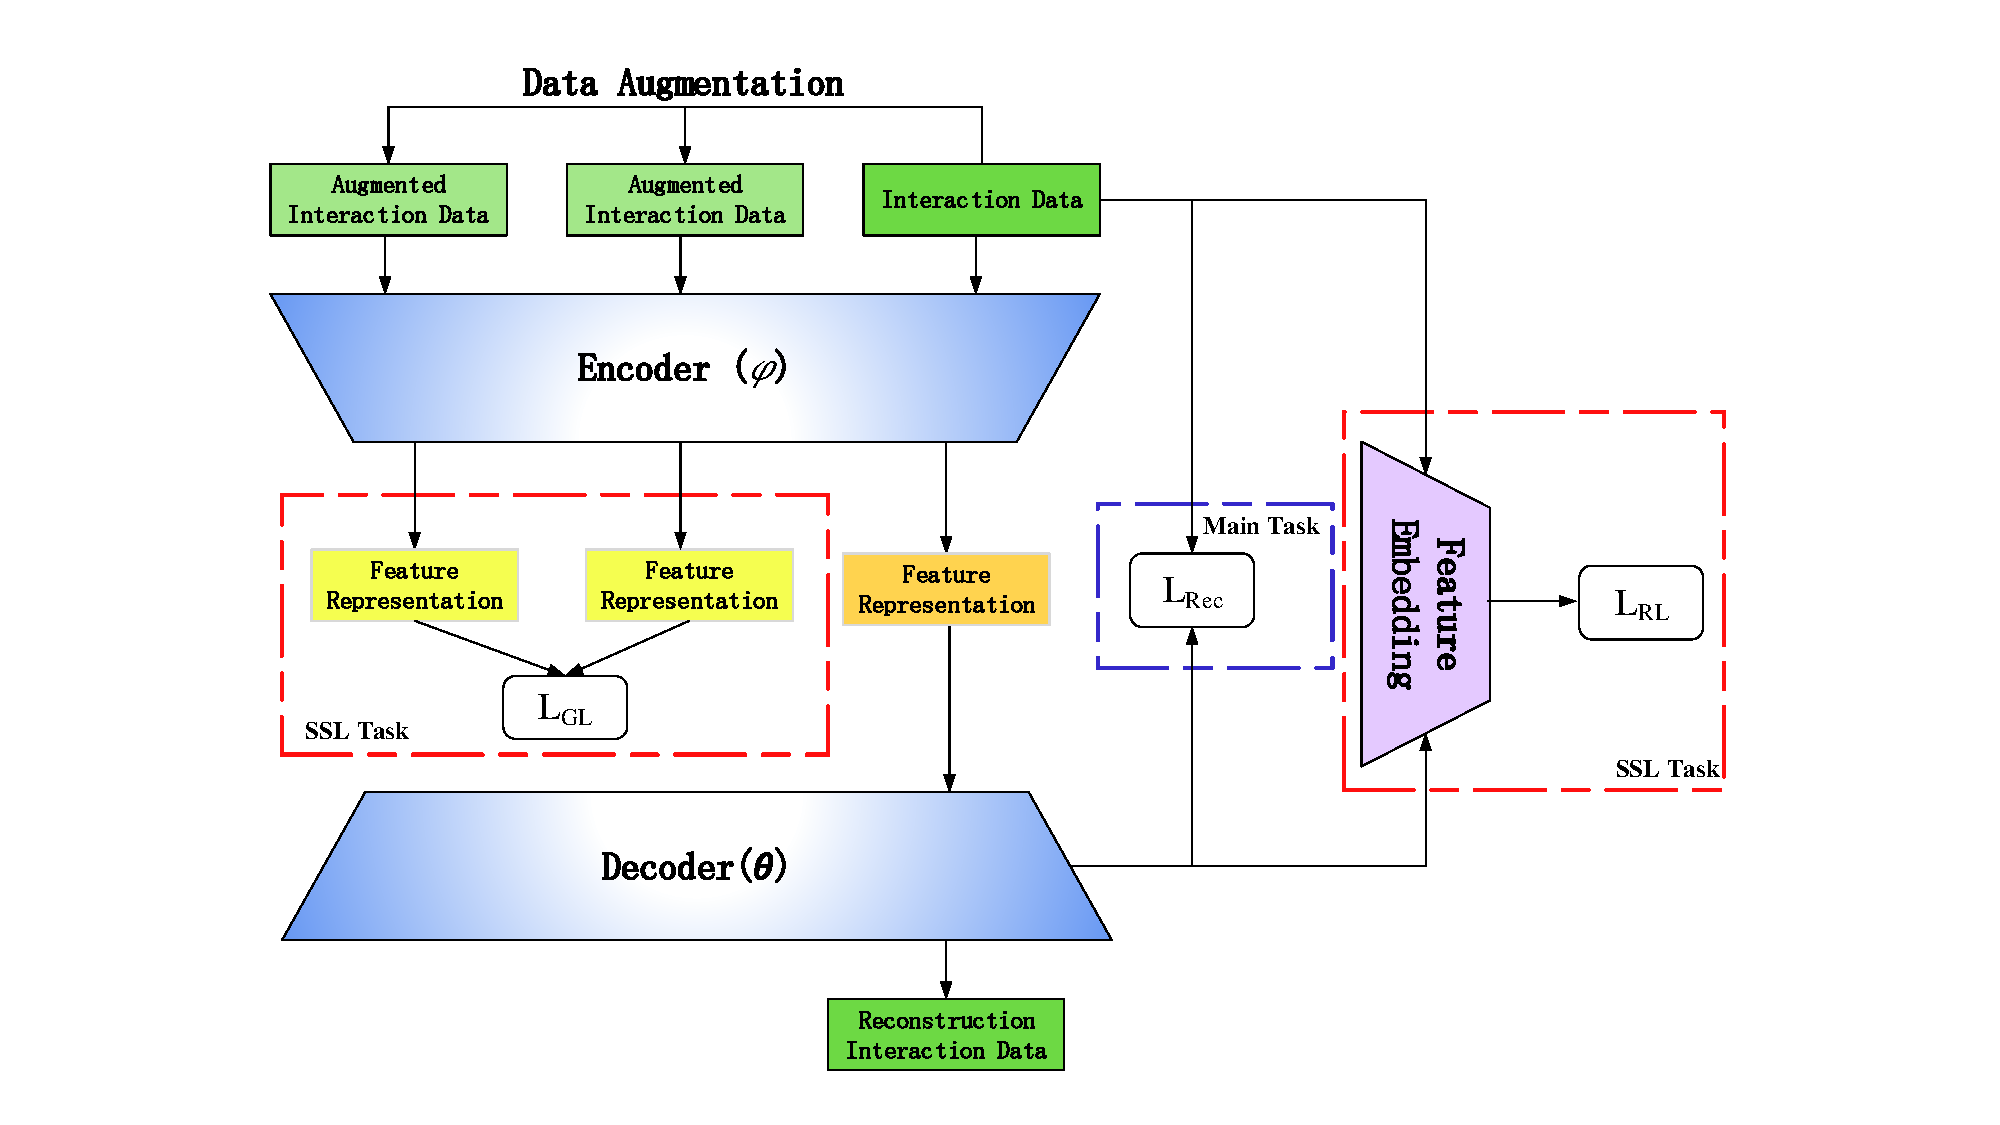
\includegraphics[width=1.2\textwidth]{fig/framework_v1.pdf}}
 \caption{ Model architecture of the proposed DSVAE algorithm.}
 % The right part presents the SSL auxiliary task,which enforces each user representation to be discriminative. And the left part illustrates main task of Top-N recommendation based on VAE.}
 \label{framework}
\end{figure*}

\section{The Proposed Method}\label{sec3}


\subsection{Notations}\label{subsec2}
In this paper, we denote scalars, vectors, and matrices using lower case, bold lower case, and bold upper case letters, e.g., $n,\mathbf{x}, \mathbf{X}$. Let $\mathbf{X}\in \mathbb{N}^{n\times m}$ denote the binary implicit feedback among $n$ users and $m$ items. Its element $x_{ij}\in \{0,1\}$ indicates whether the $j$-th item is interacted by the $i$-th user. $\mathbf{x}_i=[x_{i1}, ...,x_{im}]^\top\in\mathbb{N}^m $ is a binary vector demonstrating the click history of user $i$ on all items. The general goal of our method is to determine the feature representation $\mathbf{z}_i \in \mathbb{R}^d$ by defining some generative process from feature representation to preference feedback data,i.e., $p { \left( \mathbf{x}_i \lvert \mathbf{z}_i \right)}$. The dimensionality $d$ is usually fixed with a small value $\left(d \ll min\{n,m\}\right)$.

\subsection{Overview }\label{subsec2}
The overview architecture of the proposed DSVAE is illustrated in Fig. \ref{framework}, which is accomplish by two tasks: main supervised task and dual self-supervised task. Specially, main supervised task employs variational autoencoder to generate the user feedback data. Dual SSL task contains two SSL task for improving both the generalization ability of VAE model on the sparse interaction datasets and personalized characteristic of recommendation results. Finally, our model jointly optimizes the objective of both recommendation task and dual SSL task.

\subsection{Main task: Generating User Feedback Data }\label{33}
As depicted in Fig. \ref{framework}, in order to predict user perference, we introduce variational autoencoder to generate user feedback data, which terms as main recommendation task. Specifically, the VAE module consists of two main components: Encoder and Decoder.


\textbf{Encoder.} The encoder model takes user feedback data $\mathbf{x}_i$ as input, and transforms it into a latent feature space by parametric update functions $g_\phi$ which can output parameters $\mu \in \mathbb{R}^d $ and $\theta \in \mathbb{R}^d$ for Gaussian distribution. In our framework, $g_\phi$ is designed as multi-layer perceptrons (MLPs), and the inference of $\mathbf{z}_i$ for the corresponding $\mathbf{x}_i$ is performed as:

%learn the distribution of feature representation $\mathbf{z_u}$. approximates the true intractable posterior distribution $p(\mathbf{z_u}\lvert \mathbf{x_u})$ with a simpler variational distribution $q_\phi(\mathbf{z_u}\lvert \mathbf{x_u})$ which is assumed following a diagonal Gaussian distribution $ N(\mu,diag(\sigma^{2}))$. approximates the true intractable posterior distribution $p(\mathbf{z_u}\lvert \mathbf{x_u})$ with a simpler variational distribution $q_\phi(\mathbf{z_u}\lvert \mathbf{x_u})$.



\begin{equation}
q_\phi(\mathbf{z}_i\lvert\mathbf{x}_i)= N(\mu,diag(\sigma^{2})) \text{, with } \mu,\sigma^2=g_\phi(\mathbf{x}_i)
\label{eq1}
\end{equation}

The feature representation $\mathbf{z}_i$ is sampled from $q_\phi(\mathbf{z}_i\lvert\mathbf{x}_i)$ and then passed to the subsequent decoder layer as input.

%where $g_\phi$, known as encoder, is a neural network that outputs parameters $\mu$ and $\sigma$ for Gaussian distribution $q_\phi(\mathbf{z_u}\lvert\mathbf{x_u})$. Then the feature representation $\mathbf{z_u}$ is sampled from $q_\phi(\mathbf{z_u}\lvert\mathbf{x_u})$.

\textbf{Decoder.} In decoder layer, we suppose that reconstructed user feedback $\mathbf{x}_i$ is sampled from a generative process $p_{\theta} { \left( \mathbf{x}_i \lvert \mathbf{z}_i \right) = Mult(n,\pi(\mathbf{z}_i)) }$. The generator is a deterministic neural network $f_\theta(\mathbf{z}_i)$ parameterized by $\theta$, the output of which is normalized via a $softmax$ function to produce a probability vector $\pi\left(\mathbf{z}_i\right)$ over the entire item set.


%, which is assumed to be subject to a  multinomial distribution: $p_{\theta} { \left( \mathbf{x_u} \lvert \mathbf{z_u} \right)} = Mult(n_u,\pi(\mathbf{z_u}))$. We employ a neural network $f_\theta:\mathbb{R}^k\longrightarrow\mathbb{R}^{\lvert I \rvert}$, parameterized by $\theta$, to perform the generative process. The output of this transformation is normalized via a $softmax$ function to produce a probability vector $\pi\left(\mathbf{z_u}\right)$ over the entire item set.


\begin{equation}
\pi(\mathbf{z}_i)=softmax(f_\theta(\mathbf{z}_i))
\label{eq2}
\end{equation}
\begin{equation}
\mathbf{x}_i \sim  Mult(n_i,\pi(\mathbf{z}_i))
\label{eq3}
\end{equation}

And the log-likelihood for $\mathbf{x}_i$ is:

\begin{equation}
\log{
p_{\theta} { \left( \mathbf{x}_i \lvert \mathbf{z}_i \right) }
}=
\sum_{j}{
x_{ij}\log{
\pi_{j}\left( \mathbf{z}_i \right) 
}
 }
\label{eq4}
\end{equation}

All the above models can be trained by minimizing the negative of evidence lower bound (ELBO) in Eq. \ref{eq5} below

\begin{equation}
\begin{aligned}
\log p\left(\mathbf{x}_i;\theta\right) \geq& \mathbb{E}_{q_{\phi}\left(\mathbf{z}_i\mid\mathbf{x}_i\right)}\left[\log p_{\theta}\left(\mathbf{x}_i\mid\mathbf{z}_i\right)\right]\\ & - KL\left(q_{\phi}\left(\mathbf{z}_i\mid\mathbf{x}_i\right)\parallel P\left(\mathbf{z}_i\right)\right)\\&
\equiv \mathcal{L}_{main}\left(\mathbf{x}_i;\theta,\phi\right)\\
\label{eq5}
\end{aligned}
\end{equation}
%$\mathbb{E}_{q_{\phi}\left(\mathbf{z_u}\mid\mathbf{x_u}\right)}\left[\log p_{\theta}\left(\mathbf{x_u}\mid\mathbf{z_u}\right)\right]$
%$KL\left(q_{\phi}\left(\mathbf{z_u}\mid\mathbf{x_u}\right)\parallel P\left(\mathbf{z_u}\right)\right)$
where $P\left(\mathbf{z}_i\right)$ is the prior, which is assumed to be $N\left(0,\mathbf{I}\right)$. The first term denotes the reconstruction loss between $\mathbf{x}_i$ and $\hat{\mathbf{x}}_i$, and the second term is the KL divergence, which prevents the conditional
$q_{\phi}\left(\mathbf{z}_i\mid\mathbf{x}_i\right)$ from deviating from the Gaussian prior $N\left(0,\mathbf{I}\right)$.

\begin{algorithm}[t]
	\caption{The Algorithm of \textbf{DSVAE}}
	\begin{algorithmic}
		\label{Algorithm one}
		\STATE {\bfseries Inputs:}
		 Implicit feedback matrix $\mathbf{X}\in\mathbb{N}^{n\times m}$, hyper-parameters $\lambda_1, \lambda_2, \tau_1, \tau_2$, max training epochs: B, batch size N.\\
	%	\quad $\mathcal{X}$: The unseen instance\\
		\STATE {\bfseries Output:}
		 $\theta, \phi$

		\STATE \textbf{1.}  \textbf{while} {epoch $\leq$ B}, do\\
	    \STATE\ \quad //End-to-end optimization
	    \STATE \textbf{2.}  \quad \textbf{for} {sample mini-batch $\left\{\mathbf{x}_i\right\}_{i=1}^n$ }, do\\
		
		\STATE \textbf{3.}  \quad \quad  \textbf{for} {$\mathbf{x}\in\left\{1,2,...,n\right\}$}, do\\
		 \STATE\ \quad //Construct data augmentations
		\STATE \textbf{4.}  \quad \quad \quad $\mathbf{x}_i^{\prime} = \mathbf{P^{\prime}} \odot \mathbf{x}_i\text{,  } \mathbf{x}_i^{\prime\prime} = \mathbf{P^{\prime\prime}} \odot \mathbf{x}_i$\\
		\STATE\ \quad //Feature representation learning via inference network
		\STATE \textbf{5.}   \quad \quad \quad $q_\phi(\mathbf{z}_i\lvert\mathbf{x}_i)= N(\mu,diag(\sigma^{2}))$\\
		\STATE \textbf{6.}  \quad \quad \quad $q_\phi(\mathbf{z}_i^{\prime}\lvert\mathbf{x}_i^{\prime})= N(\mu^{\prime},diag(\sigma^{\prime 2}))$\\
		\STATE \textbf{7.} \quad \quad \quad $q_\phi(\mathbf{z}_i^{\prime\prime}\lvert\mathbf{x}_i^{\prime\prime})= N(\mu^{\prime\prime},diag(\sigma^{\prime\prime 2}))$\\
		 \STATE\ \quad //generating reconstruction via generation network
		\STATE \textbf{8.}  \quad\quad \quad $\log{p_{\theta} { \left( \mathbf{x}_i \lvert\mathbf{z}_i\right)}}=\sum_{j}{x_{ij}\log{\pi_{j}\left( \mathbf{z}_i \right) }}$
		\STATE \textbf{9.}  \quad \quad \textbf{end for}
		\STATE\ \quad //Multi-Task optimization
		\STATE \textbf{10.}  \quad  \quad  $\mathcal{L} = \mathcal{L}_{main} + \lambda_1 \mathcal{L}_{gcl} + \lambda_1 \mathcal{L}_{rcl}$\\
		\STATE \textbf{11.} \quad  \quad Update $\theta$ and $\phi$ of VAE to minimize $\mathcal{L}$;
		\STATE \textbf{12.} \quad \textbf{end for}
		\STATE \textbf{13.} \textbf{end while}
		%\quad $\mathcal{Y}$: The Final Predicted Label;\\
	\end{algorithmic}
\end{algorithm}


                 
           

\subsection{Dual Self-supervised Learning Task}\label{23-}
As illustrated in Fig. \ref{framework}, self-supervised learning is introduced to improve both the generalization ability of VAE model on the sparse interaction datasets and personalized characteristic of recommendation results. Thus, two SSL task are defined as follows: %$1)$ Generating different views of user feedback by data augmentation and maximizing agreement between two augmented views of one user compared to that of other users; $2)$ Encouraging the matching between reconstruction user feedback $\hat{\mathbf{x}}_u$ and input user feedback $\mathbf{x_u}$, while pushing the $ \mathbf{\hat{x}_u}$ away from the rest of user feedback.



\textbf{Generalization ability enhancing self-supervised learning task.}\label{231}  
In order to enhance the generalization ability of VAE, we construct SSL task which aligns the representations learned from different views. The SSL task includes two procedures: data augmentation and contrastive learning, respectively.

%General contrastive self-supervised learning method requires transforming input data (via data augmentation operations) to generate new training data for constructing pertask. 
%Thus, we augment user feedback data in training set to obtain two views of one user. With augmented views, we conduct contrastive learning to align the representations learned from different views.



(1) \textbf{Data Augmentation.} Given user history interaction, the key idea is to create two augmented examples by masking part of user interaction. With this operation, we term different augmented examples as different views for the same user interaction, in which case our method can explore internal correlation between them. For each user feedback vector, we can randomly mask the value of positive items with a ratio $\alpha$, which can be expressed as follows:

\begin{equation}
\mathbf{X^{\prime}} = \mathbf{P^{\prime}} \odot \mathbf{X}\text{,  } \mathbf{X^{\prime\prime}} = \mathbf{P^{\prime\prime}} \odot \mathbf{X}
\label{eq6}
\end{equation}

where $\mathbf{P^{\prime}},\mathbf{P^{\prime\prime}}\in\left\{ \ 0,1 \right\}^{\lvert m \rvert}$ are independent masking vectors which are applied on feedback matrix $\mathbf{X}$ to generate two augmented views $\mathbf{X}^{\prime}$ and $\mathbf{X}^{\prime\prime}$. As such, this augmentation operation is expected to learn internal relationship between $\mathbf{X}^{\prime}$ and $\mathbf{X}^{\prime\prime}$.

(2) \textbf{Contrastive Learning.} With augmented views $\mathbf{X}^{\prime}$ and $\mathbf{X}^{\prime\prime}$,  we further employ contrastive learning to align the representations $\mathbf{z}_i^{\prime}$ and $\mathbf{z}_i^{\prime\prime}$ which are learned from different views. % by minimizing contrastive loss.
Here, we treat $\{(\mathbf{x}_i^{'},\mathbf{x}_i^{''}) \mid i \in \mathbf{U}\}$ as positive pair and
$\{(\mathbf{x}_i^{'},\mathbf{x}_j^{''}) \mid i,j \in \mathbf{U}, i \neq j\}$ as negative pair, where $\mathbf{U}$ is the set of users. To encourage the above properties, contrastive loss is represented as


\begin{equation}
\mathcal{L}_{gcl} = \sum_{i\in U}-\log\frac{\exp(s(\mathbf{z}_i^{'},\mathbf{z}_i^{''})/\tau_1)}{\sum_{j\in \mathbf{U}} \exp(s(\mathbf{z}_i^{'},\mathbf{z}_j^{''})/\tau_1)}
\label{eq7}
\end{equation}

\begin{equation}
\mathbf{Z}^{\prime} = g_{\phi}\left(\mathbf{X}^{\prime}\right), \mathbf{Z}^{\prime\prime}=g_{\phi}\left(\mathbf{X}^{\prime\prime}\right)
\label{eq8}
\end{equation}


where $g_{\phi}$ is encoder network mentioned in Section \ref{33}  which serves to learn feature representations matrix $\mathbf{Z}^{\prime}$ and $\mathbf{Z}^{\prime\prime}$. $s(\cdot) $ is cosine similarity, $\tau_1$ is a tunable hyper-parameter for the softmax temperature.  
By minimizing contrastive loss, $\mathbf{z}_i^{\prime}$ is enforce to be more similar to positive sample $\mathbf{z}_i^{\prime\prime}$ than other negative samples $\mathbf{z}_j^{\prime}$. 

\textbf{Personalized characteristic enhancing self-supervised learning task.} Unlike contrastive learning method mentioned above, which generates positive pair by data augmentation, the reconstruction and input matrix of VAE naturally fit into the contrastive term. To be specific, given user feedback matrix $\mathbf{X}$ and its reconstruction $\hat{\mathbf{X}}\in \mathbb{N}^{n\times m}$, we separately take  $\{(\hat{\mathbf{x}}_i,\mathbf{x}_i) \mid i \in \mathbf{U}\}$ as positive pair and $\{(\hat{\mathbf{x}}_i,\mathbf{x}_j) \mid i,j \in \mathbf{U}, i \neq j\}$ as negative pair. 
 

Then contrastive learning is adopted to optimize VAE by maximizing the agreement between user feedback vector and its own reconstruction. It encourages reconstruction to be as close as possible to the corresponding user feedback while being different from all rest user feedback. The contrastive loss is defined as,

\begin{equation}
\mathcal{L}_{rcl} = \sum_{i\in U}-\log\frac{\exp(s(h\left(\hat{\mathbf{x}}_i\right),h\left(\mathbf{x}_i\right)/\tau_2)}{\sum_{j\in \mathbf{N}_i} \exp(s(h\left(\hat{\mathbf{x}}_i\right),h\left(\mathbf{x}_j\right))/\tau_2)}
\label{eq9}
\end{equation}

here $h(\cdot)$ is designed as multi-layer perceptrons to extra feature embedding. $\mathbf{N}_i$ is negative sample set, $s(\cdot) $ is cosine similarity and $\tau_2$ is a tunable hyper-parameter for the softmax temperature. 

As  such, minimizing $\mathcal{L}_{rcl}$ can lead to more personalized recommendation result, i.e. distinguishing each reconstruction different from the others.

\subsection{Optimizing Multi-task Learning}\label{35}
%\subsubsection{Multi-task Training}\label{subsubsec2}
To enable SSL strategy learned representation to boost main recommendation performance, we optimize a combined objective of recommendation task and pretext task,
%we leverge a multi-task strategy to optimize them jointly. Intuitively, a linear weighted sum approach is as follows:


\begin{equation}
\mathcal{L} = \mathcal{L}_{main} + \lambda_1 \mathcal{L}_{gcl} + \lambda_2 \mathcal{L}_{rcl}
\label{eq10}
\end{equation}
here $\mathcal{L}_{gcl}$ and $\mathcal{L}_{rcl}$ are defined respectively in Eq.(\ref{eq7}) and Eq.(\ref{eq9}); $\lambda_1$ and $\lambda_2$ are hyper-parameters to control the strength of contrastive SSL loss; $\mathcal{L}_{VAE}$ is defined in Eq.(\ref{eq5}); 

The algorithmic framework of our proposed DSVAE method is given in Algorithm \ref{Algorithm one}. We randomly initialize parameters of encoder, decoder and feature embedding layer. A training epoch consists of two tasks: main recommendation task and dual SSL task.


\section{Experiment}\label{sec4}
In this section, we evaluate the proposed DSVAE model on three datasets by comparing with state-of-the-art methods.


\begin{table}
    %\renewcommand\arraystretch{1.0}
    \begin{center}
    \caption{Statistics of three datasets.} \label{tab1}
    \setlength{\tabcolsep}{2.5mm}{
    \begin{tabular}{cccccc}
     %   \toprule
        \hline \hline
          \textbf{Datasets} & \textbf{ML-1M}   & \textbf{Douban Book} & \textbf{Epinions}\\
          \hline
       % \midrule
          Users   & 6,040     & 13,024  & 18,088\\
          Items   & 3,706     & 22,347  & 261,649\\
          Ratings & 1,000,209 & 792,062 & 764,352\\
          Density & 2.7\%     & 0.255\% & 0.019\%\\
          User Information  & Age, Gender, Occupation &$*$           & $*$                      \\
        \hline \hline
      %   \bottomrule
    \end{tabular}}
    \end{center}
\end{table}

\subsection{Experimental Setup}\label{41}
To comprehensively and effectively evaluate the performance of our proposed DSVAE approach, we conduct experiments on three real-world datasets: 
\begin{itemize}
\item ML-1M \cite{DBLP:journals/tiis/HarperK16}: ML-1M collects user-movie interaction data from movie domain, and contains 6,040 users, 3,706 items and 1,000,209 ratings which are 10 discrete numbers within range of $\left[0.5,5\right]$ and density of ratings is 2.7\%.
User content information is also included, i.e., age, gender, occupation.

%\item ML-20M \cite{DBLP:conf/recsys/MassaA07}: ML-20M is a different scale of ML datasets. It contains 136,677 users, 22,347 items and 9,990,682 ratings which are 5 discrete numbers within range of $\left[1,5\right]$ and density of ratings is 0.353\%.

\item Douban Book \cite{DBLP:journals/tmm/ZhaoQX16}: Douban is the largest book review website in China, where user can rate or review books. It includes 13,024 users, 22,347 items and 792,062 ratings which are 5 discrete numbers within range of $\left[1,5\right]$ and density of ratings is 0.255\%.

\item Epinions \cite{DBLP:conf/recsys/MassaA07}:
Epinions is extracted from consumer review website Epinions. It contains 18,088 users, 261,649 items and 764,352 ratings which are 5 discrete numbers within range of $\left[1,5\right]$ and density of ratings is 0.019\%.

\end{itemize}

Table \ref{tab1} summarizes the characteristics of these employed experimental datasets. All the datasets are processed following \cite{DBLP:conf/www/LiangKHJ18}. We binarize explicit data by keeping ratings of four and higher and reserve users who have bought or rated at least five items.


%\textbf{Metrics:}
Two widely used collaborative filtering evaluation metrics are adopted for performance comparisons, i.e., Recall and NDCG.

\begin{itemize}
\item Recall: Recall ratio of the ground truth item. Recall is used to test whether recommendation item is in the top-K list. 

\begin{equation}
\mathbf{Recall}@k(i) = \frac{\lvert \mathbf{R}_i \cap \mathbf{T}_i \rvert }
{\lvert \mathbf{T}_i \rvert}
\label{eq11}
\end{equation}

Here, $\mathbf{R}_i$ stands for the set of recommender items to user $i$. It's obtained by sorting likelihood of items which is predicted by decoder in VAE, excluding items from the training set. $\mathbf{T}_i$ denotes the set of favorite items of user $u$.

\item NDCG: Normalized Discounted Cumulative Gain (NDCG)  is adopted to measure the item ranking accuracy which assigns higher scores to top ranked items to consider the position of correctly recommended items.


\begin{equation}
\mathbf{NDCG} @k\left(i\right) = \frac{ \mathbf{DCG}@k\left(i\right)
 }{\mathbf{IDCG}@k\left(i\right)}
 \label{eq12}
\end{equation}

\begin{equation}
\mathbf{DCG}@k(i) = \sum_{n=1}^k \frac{ 2^{\mathbbm{1} \left( \mathbf{R}_i  \in \mathbf{T}_i\right)}-1}
{\log\left(\mathbf{n+1} \right)}
\label{eq13}
\end{equation}

where IDCG is the DCG value with perfect ranking, $\mathbf{R}_i$ denotes the set of recommendation items to user $i$ and $\mathbf{T}_i$ denotes the set of favorite items of user $i$, $\mathbbm{1}$ is the indicator 
function.
\end{itemize} 




\begin{table}
    %\renewcommand\arraystretch{1.0}
    \begin{center}
    \caption{Performance comparison with several rating-only VAE based CF models.} \label{tab2}
   % \linespread{2.5} 
    \renewcommand\arraystretch{1.5}
    \setlength{\tabcolsep}{2mm}{
\begin{tabular}{ccccccc}
%\begin{tabular}{ccccccc}
\hline\hline
Data                          & Metric    & Mult-VAE & Improve & RecVAE & Improve & DSVAE  \\ \hline
\multirow{4}{*}{Douban Book}  & NDCG@25   & 0.1321   & 19.9\%  & 0.1418 & 11.7\%  & \textbf{0.1584} \\
                              & NDCG@50   & 0.1530   & 16.1\%  & 0.1633 & 8.8\%   & \textbf{0.1776} \\
                              & Recall@25 & 0.1785   & 8.7\%   & 0.1771 & 9.5\%   & \textbf{0.1940} \\
                              & Recall@50 & 0.2383   & 4.7\%   & 0.2418 & 3.2\%   & \textbf{0.2495} \\ \hline
\multirow{4}{*}{ML-1M} & NDCG@25   & 0.2977   & 17.8\%  & 0.3224 & 8.8\%   & \textbf{0.3507} \\
                              & NDCG@50   & 0.3388   & 13.5\%  & 0.3773 & 2.0\%   & \textbf{0.3847} \\
                              & Recall@25 & 0.3532   & 14.2\%  & 0.3842 & 5.0\%   & \textbf{0.4032} \\
                              & Recall@50 & 0.4602   & 8.3\%   & 0.4939 & 1.0\%   & \textbf{0.4982} \\ \hline
\multirow{4}{*}{Epinions}     & NDCG@25   &\textbf{0.0466}          & -10.6\%  &0.0346        & 21.7\%  & 0.0421        \\
                              & NDCG@50   &\textbf{0.0564}          & -10.0\%  & 0.0422        & 20.8\%  & 0.0510        \\
                              & Recall@25 & \textbf{0.0845}          & -11.7\%   & 0.0648       & 16.7\%   & 0.0756        \\
                              & Recall@50 & \textbf{0.1217}          & -10.1\%   & 0.0929       & 18.9\%   & 0.1105        \\ \hline \hline


\end{tabular}}
\end{center}
\end{table}


%\textbf{Baselines:} 
We compare the proposed approach with four state-of-the-art methods, including two interaction-only VAE based recommendation approaches, and two content-aware VAE based recommendation approaches. Interaction-only VAE based recommendation approaches including Mult-VAE and RecVAE which are frequently used as comparison algorithms in VAE based CF methods. Content-aware VAE based recommendation approaches including  Split-Merge CVAE and JVAE-CF which use side information to alleviate data sparsity problem. We demonstrate the effectiveness of SSL by comparing with content-aware VAE models.


%Mult-VAE is classical VAE based approach, RecVAE is the best performance VAE based approach. 
%They are frequently used as comparison algorithms in VAE based collaborative filtering method. Content-aware VAE based recommendation approaches including  Split-Merge CVAE and JVAE-CF which use content information to alleviate data sparsity. 


For all comparison methods, we use the source code provided by the corresponding authors to reproduce experiment result or directly adopt best result presented in original paper.


\begin{itemize}
\item Mult-VAE \cite{DBLP:conf/www/LiangKHJ18}: A typical VAE based CF approach, which applies variational autoencoder model with multinomial likelihood to approximate recommendation ranking loss and improves the predictive performance. And it uses Bayesian inference for parameter estimation.

\item Rec-VAE \cite{DBLP:conf/wsdm/ShenbinATMN20}: A complex variant of Mult-VAE, which proposes a new approach to set $\beta$ hyper-parameter for Kullback-Leibler term in objective function and replaces Gaussian distribution prior with composite distribution prior. The composite distribution prior is a mixture of standard Gaussian prior and feature representation distribution.  


\item Split-Merge CVAE \cite{DBLP:conf/pakdd/PangYW19}: An conditional variational autoencoder which concentrates on
learning with label verification signals to ensure an exclusive latent mean factor for users with the same labels and leverages split-merge framework to handle complex multi-label combinations. Content information aims to promote model to distinguish and cluster users in latent subspace.

\item JVAE-CF \cite{DBLP:conf/cikm/LeeSM17}: JVAE-CF encompasses VAE through augmenting structures to model both content information and user interaction information, which adds additional latent variable to extract high-level features associated with auxiliary information.
\end{itemize}

Moreover, to verify the effectiveness of each component used by DSVAE, a series of degenerate variants of DSVAE are also included for the comparisons:

\begin{itemize}
\item DSVAE-wGL: A degenerate variant of DSVAE. The difference between DSVAE-wGL and DSVAE is that the former does not use generated data to construct $\mathcal{L}_{gcl}$
\item DSVAE-wRL: A weak version of DSVAE and an upgraded version of RecVAE, which omits $\mathcal{L}_{rcl}$ loss.
\end{itemize}

%\textbf{Implementation Details:}
The parameters of all baselines are adopted from their original papers. 
As for DSVAE method, we take RecVAE as the VAE model and inherit the optimal values of hyper-parameters from RecVAE. For the unique part of DSVAE, we fine-tuned dual SSL task hyper-parameters to achieve best performance. In detail, the softmax temperature $\tau_1$ and $\tau_2$, the number of negative sample $\mathbf{N}_i$ and dropout ratio $\alpha$ is discussed in Section \ref{45}. DSVAE is implemented in PyTorch, the optimizer is Adam and hyper-parameters are automatically tuned according to the TPE method.


 %Before conducting the experiments, we give the range of the required variables. In detail, the softmax temperature $\tau_1$ and $\tau_2$ are set among $\left\{0.1, 0.3,...,0.9\right\}$ to make node representations more discriminative. The coefficient parameter $\lambda_1$ and $\lambda_2$ are chosen from $\left\{0, 0.01, 0.05, 0.1, 0.2\right\}$ to balance the effect of dual SSL task. The number of negative sample $\mathbf{N}_i$ is set to 80 for ML-1M, 128 for Douban Book and 150 for Epinions. The dropout ratio $\alpha$ is set to 0.5. DSVAE is implemented in PyTorch, the optimizer is Adam and hyper-parameters are automatically tuned according to the TPE method.



\subsection{Performance comparison with several interaction-only VAE based CF models}\label{subsec2}
We compare our DSVAE with two interaction-only VAE based CF methods (Mult-VAE, Rec-VAE), and the corresponding quantitative results in terms of NDCG and Recall are tabulated in Table \ref{tab2}, where the best performance is boldfaced and percentage indicates the relative improvement of our approach over other compared methods.

As shown in Table \ref{tab2}, our proposed model achieves 0.3847 in terms of NDCG@25, which is respectively 8.8\% and 17.8\% superior over RecVAE and Mult-VAE on ML-1M dataset. And our proposed model achieves 0.1418 in terms of NDCG@25 , which is respectively 19.9\% and 11.7\% superior over RecVAE and Mult-VAE on Douban Book dataset. However, the performance of RecVAE on Epinion datasets is worse than Mult-VAE so that DSVAE is not as good as Mult-VAE. The experiments mentioned above powerfully demonstrate the effectiveness of DSVAE, and we attribute the success to the superiority of dual self-supervised task. Particularly, we observe that improvements on Douban Book and Epinions are more significant than ML-1M. This might be caused by data characteristics. Specifically, in Douban Book and Epinions, user-item interaction data is too sparse to guide the feature representation learning in VAE, while benefiting from the self-supervised learning task, DSVAE obtains auxiliary supervisions information to assist the feature representation learning.




\begin{table}
    %\renewcommand\arraystretch{1.0}
    \begin{center}
    \caption{Performance comparison with content aware VAE based CF models on dataset ML-1M.}\label{tab3}
    \setlength{\tabcolsep}{2.0mm}{
    \begin{tabular}{cccccc}
        \hline \hline
          \textbf{Model}  & \textbf{JVAE-CF} &\textbf{Improve}  &\textbf{Split-Merge CVAE} &\textbf{Improve}  &\textbf{DSVAE}\\\hline

          NDCG@25  &0.2963 &7.1\% &0.2905 & 9.2\% &\textbf{0.3171}\\
          NDCG@50  &0.2794 &27.8\% &0.2543 &40.5\% &\textbf{0.3572}\\
          Recall@25  &0.3423 &4.5\% &\textbf{0.3750} &-4.6\% & 0.3577\\
          Recall@50  & 0.4256  & 9.7\%   & 0.4500           & 3.8\%   & \textbf{0.4669}\\ \hline\hline
       
    \end{tabular}}
    \end{center}
\end{table}
\subsection{Performance comparison with content aware VAE based CF models}\label{subsec2}
Next, we compare our DSVAE with two content aware VAE based CF methods (Split-Merge CVAE, JVAE-CF) on ML-1M which contains user information. For fair comparison, we conduct DSVAE with the same backbone as Split-Merge CVAE and JVAE-CF. The experiment results are summarized in Table \ref{tab3}. %, where the best performance is boldfaced and percentage indicates the relative improvement of our approach over other compared methods. 
We can find that DSVAE outperforms Split-Merge CVAE and JVAE-CF. It is worth noting that Split-Merge CVAE and JVAE-CF exploits both interaction data and content information, while DSVAE only uses interaction data. This observation demonstrates that DSVAE can add additional supervised information which is as useful as content information.
\begin{table} 
    %\renewcommand\arraystretch{1.0}
    \begin{center}
    \caption{Performance of our proposed DSVAE model with DSVAE-wRL,DSVAE-wCL and RecVAE with the evaluation metric NDCG@{25,50}, Recall@{25,50} on ML-1M, Douban Book and Epinions Datasets.}\label{tab4}
     \renewcommand\arraystretch{1.5}
    \setlength{\tabcolsep}{2.0mm}{
    
\begin{tabular}{ccccccc}
\hline
Data                          & Metric    & RecVAE & DSVAE-wrcl & DSVAE-wgcl & DSVAE   \\ \hline\hline
\multirow{4}{*}{Douban Book}  & NDCG@25   & 0.1418   & 0.1516  & 0.1532 & \textbf{0.1584}   \\
                              & NDCG@50   & 0.1633   & 0.1772  & 0.1741    & \textbf{0.1776} \\
                              & Recall@25 & 0.1771   & 0.1881   & 0.1855   & \textbf{0.1940} \\
                              & Recall@50 & 0.2418   & 0.2476   & 0.2462   & \textbf{0.2495} \\ \hline
\multirow{4}{*}{ML-1M} & NDCG@25   & 0.3224   & 0.3418  & 0.3465   & \textbf{0.3507} \\
                              & NDCG@50   & 0.3773   & 0.3776  & 0.3834   & \textbf{0.3847} \\
                              & Recall@25 & 0.3842   & 0.3979  & 0.3886   & \textbf{0.4032} \\
                              & Recall@50 & 0.4939   & 0.5003   & 0.4911   & \textbf{0.4982} \\ \hline
\multirow{4}{*}{Epinions}     & NDCG@25   & 0.0346           & 0.0384       & 0.0378  & \textbf{0.0421}       \\
                              & NDCG@50   & 0.0422           & 0.0470       &0.0474   & \textbf{0.0510}       \\
                              & Recall@25 & 0.0648            & 0.0672       &0.0669   & \textbf{0.0756}        \\
                              & Recall@50 & 0.0929            &  0.0999      &0.1037    & \textbf{0.1105}       \\ \hline \hline
       
    \end{tabular}}
    \end{center}
\end{table}



\subsection{Ablation Experiments}\label{subsec2}
In this section, we conduct an ablation study on DSVAE to further analyze the contribution of two SSL tasks. 
Specifically, we compare our proposed DSVAE method with RecVAE, DSVAE-wgcl and DSVAE-wrcl. The performance comparison is shown in Table \ref{tab4}. We have the following observations:


\textbf{Effect of $\mathcal{L}_{gcl}$:} To illustrate the effect of $\mathcal{L}_{gcl}$ in VAE based recommendation task, we first make comparison between DSVAE and DSVAE-wgcl on three real-world data sets. As shown in Table \ref{tab4}, DSVAE significantly outperforms DSVAE-wgcl on three datasets, which shows that our proposed $\mathcal{L}_{gcl}$ is effective for VAE based recommendation models. Exploring correlation between two fractions of the same user interaction is beneficial to learn a better feature representation. In addition, DSVAE-wrcl outperforms RecVAE even without $\mathcal{L}_{rcl}$. This observation illustrates the superiority of our $\mathcal{L}_{gcl}$ contrastive loss in VAE based recommendation models.

\textbf{Effect of $\mathcal{L}_{rcl}$:} To demonstrate the necessity of $\mathcal{L}_{rcl}$, we compare DSVAE with DSVAE-wRC and DSVAE-wgcl with RecVAE. From Table \ref{tab4}, we observe that DSVAE outperforms DSVAE-wrcl on three datasets, which verifies the effectiveness of $\mathcal{L}_{rcl}$. Besides, by comparing RecVAE with DSVAE-wgcl, we find the latter outperforms the former significantly, which also verifies the superiority of our proposed $\mathcal{L}_{rcl}$.

%By comparing RecVAE, DSVAE, DSVAE-wgcl, DSVAE-wrcl, we find that whether improvement of $\mathcal{L}_{gcl}$ and $\mathcal{L}_{rcl}$ will boost performance of RecVAE. Particularly, DSVAE-wrcl obtains more performance gain than DSVAE-wgcl on denser datasets such as ML-1M and DSVAE-wrcl performs worse than DSVAE-wgcl on sparser dataset such as Douban Book. This observation indicates that our proposed $\mathcal{L}_{gcl}$ benefit more in a more sparser ratings situation.

\begin{figure*}[!htb]
\centering
\subfigure[Effect of $\tau_1$ (temperature hyper-parameter) ]
{\label{lambda}
    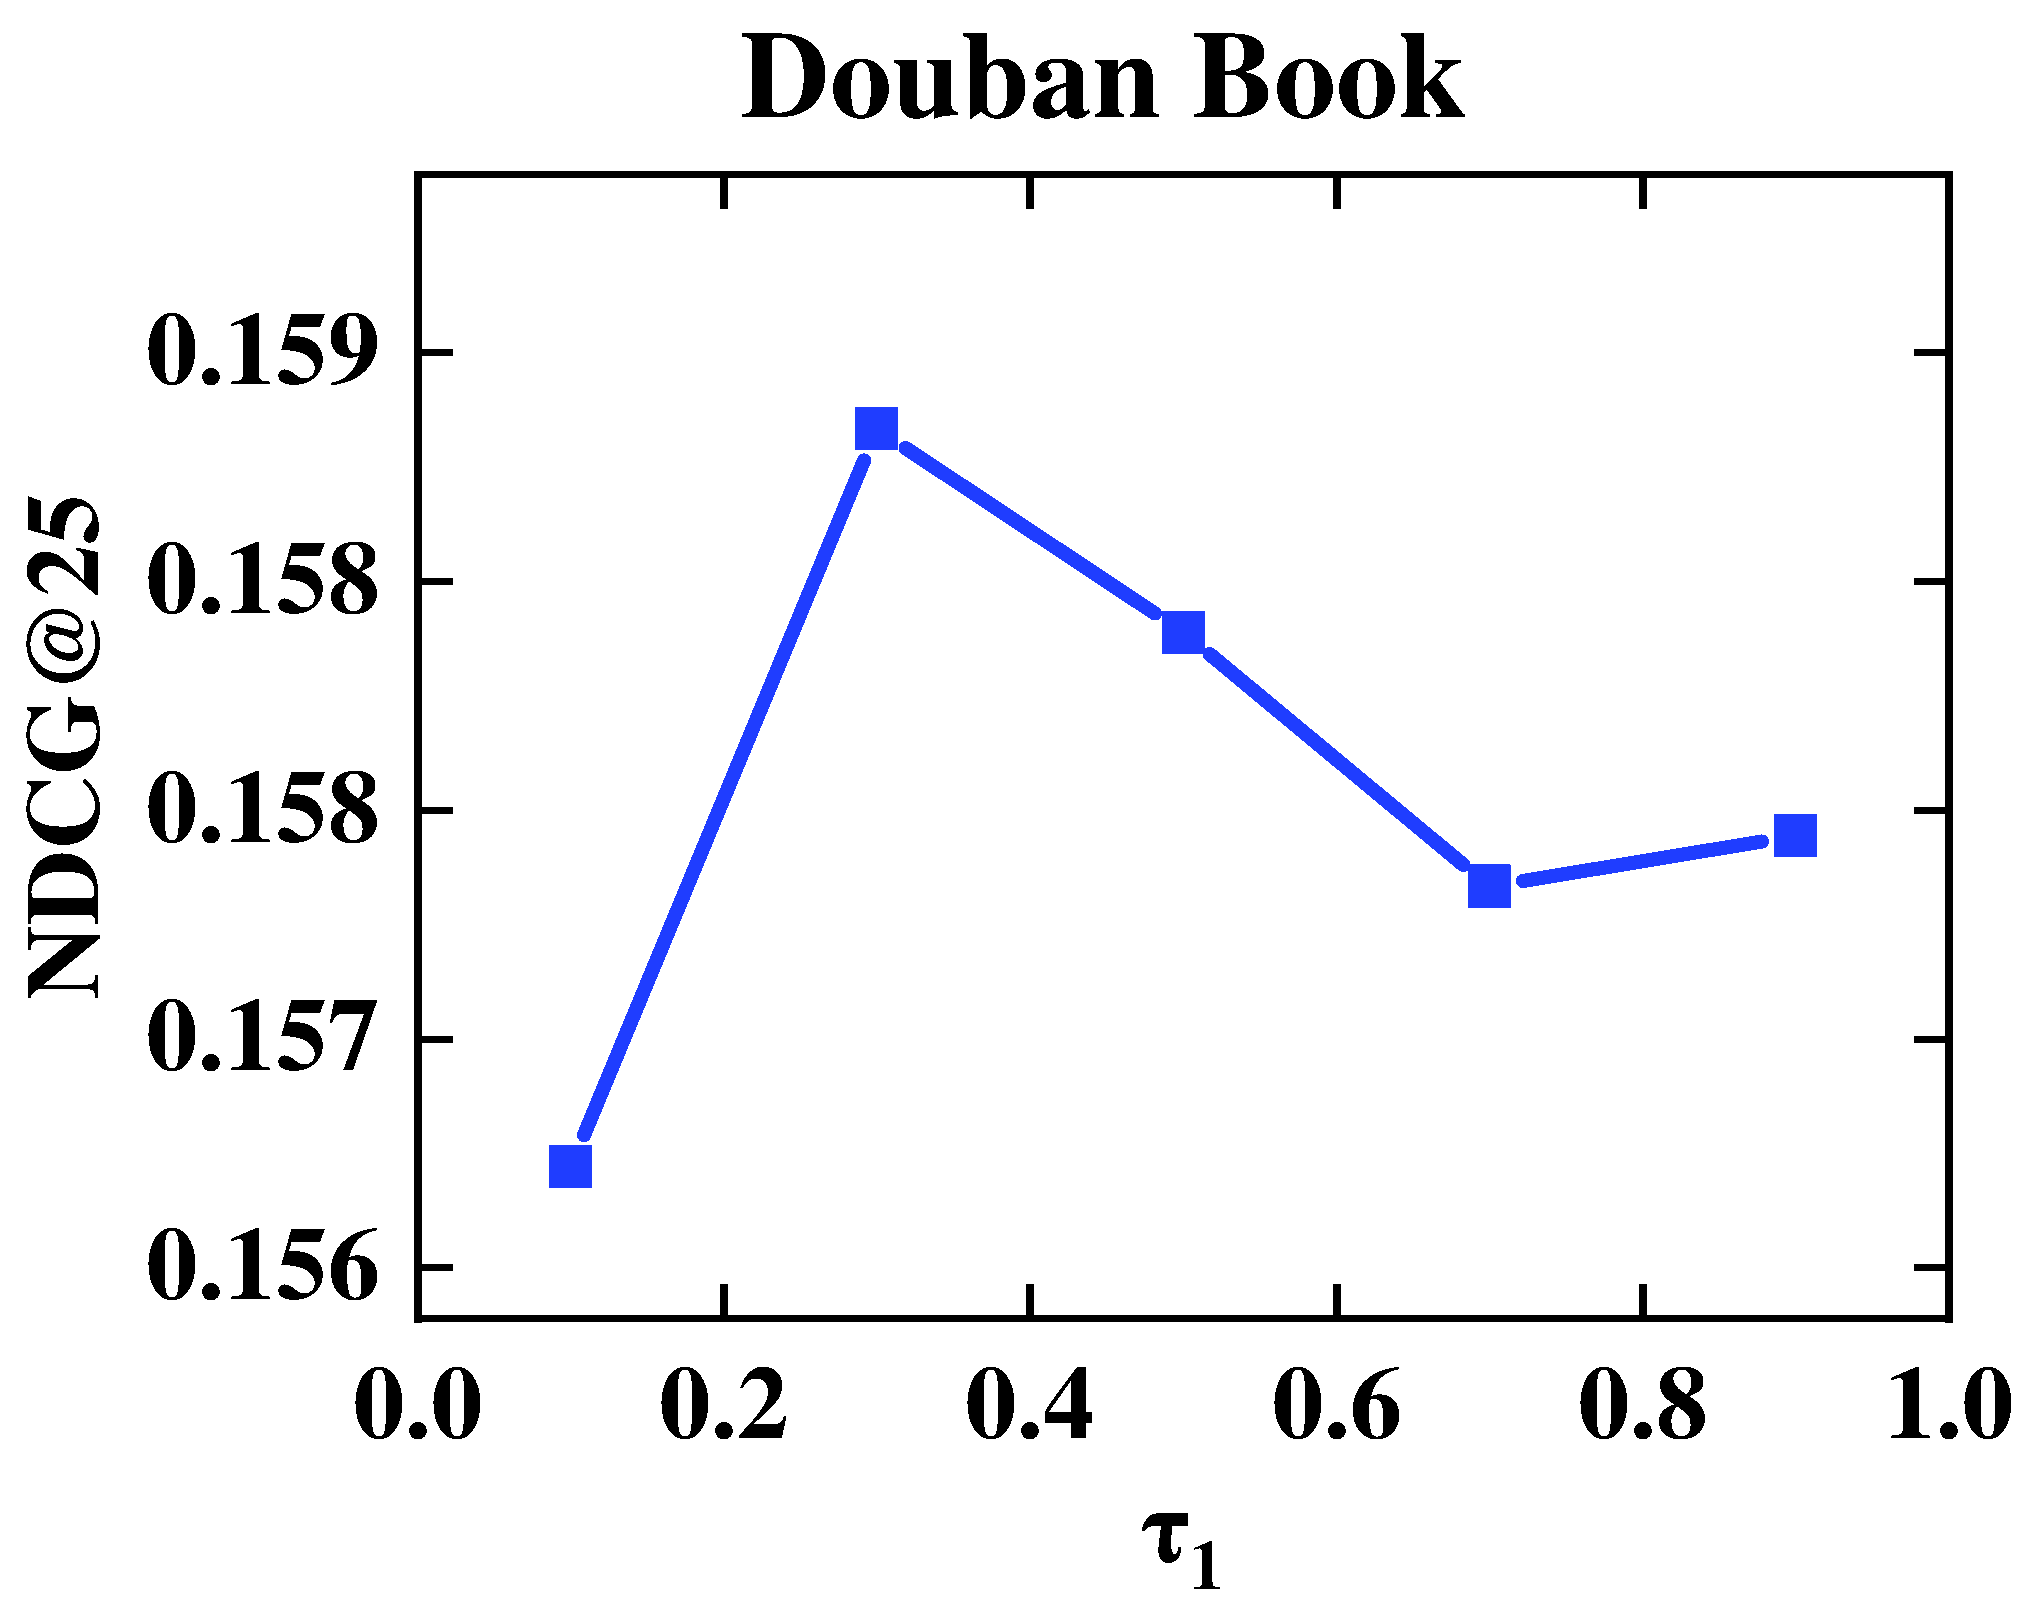
\includegraphics[width=0.25\textwidth]{fig/par/1.pdf}
    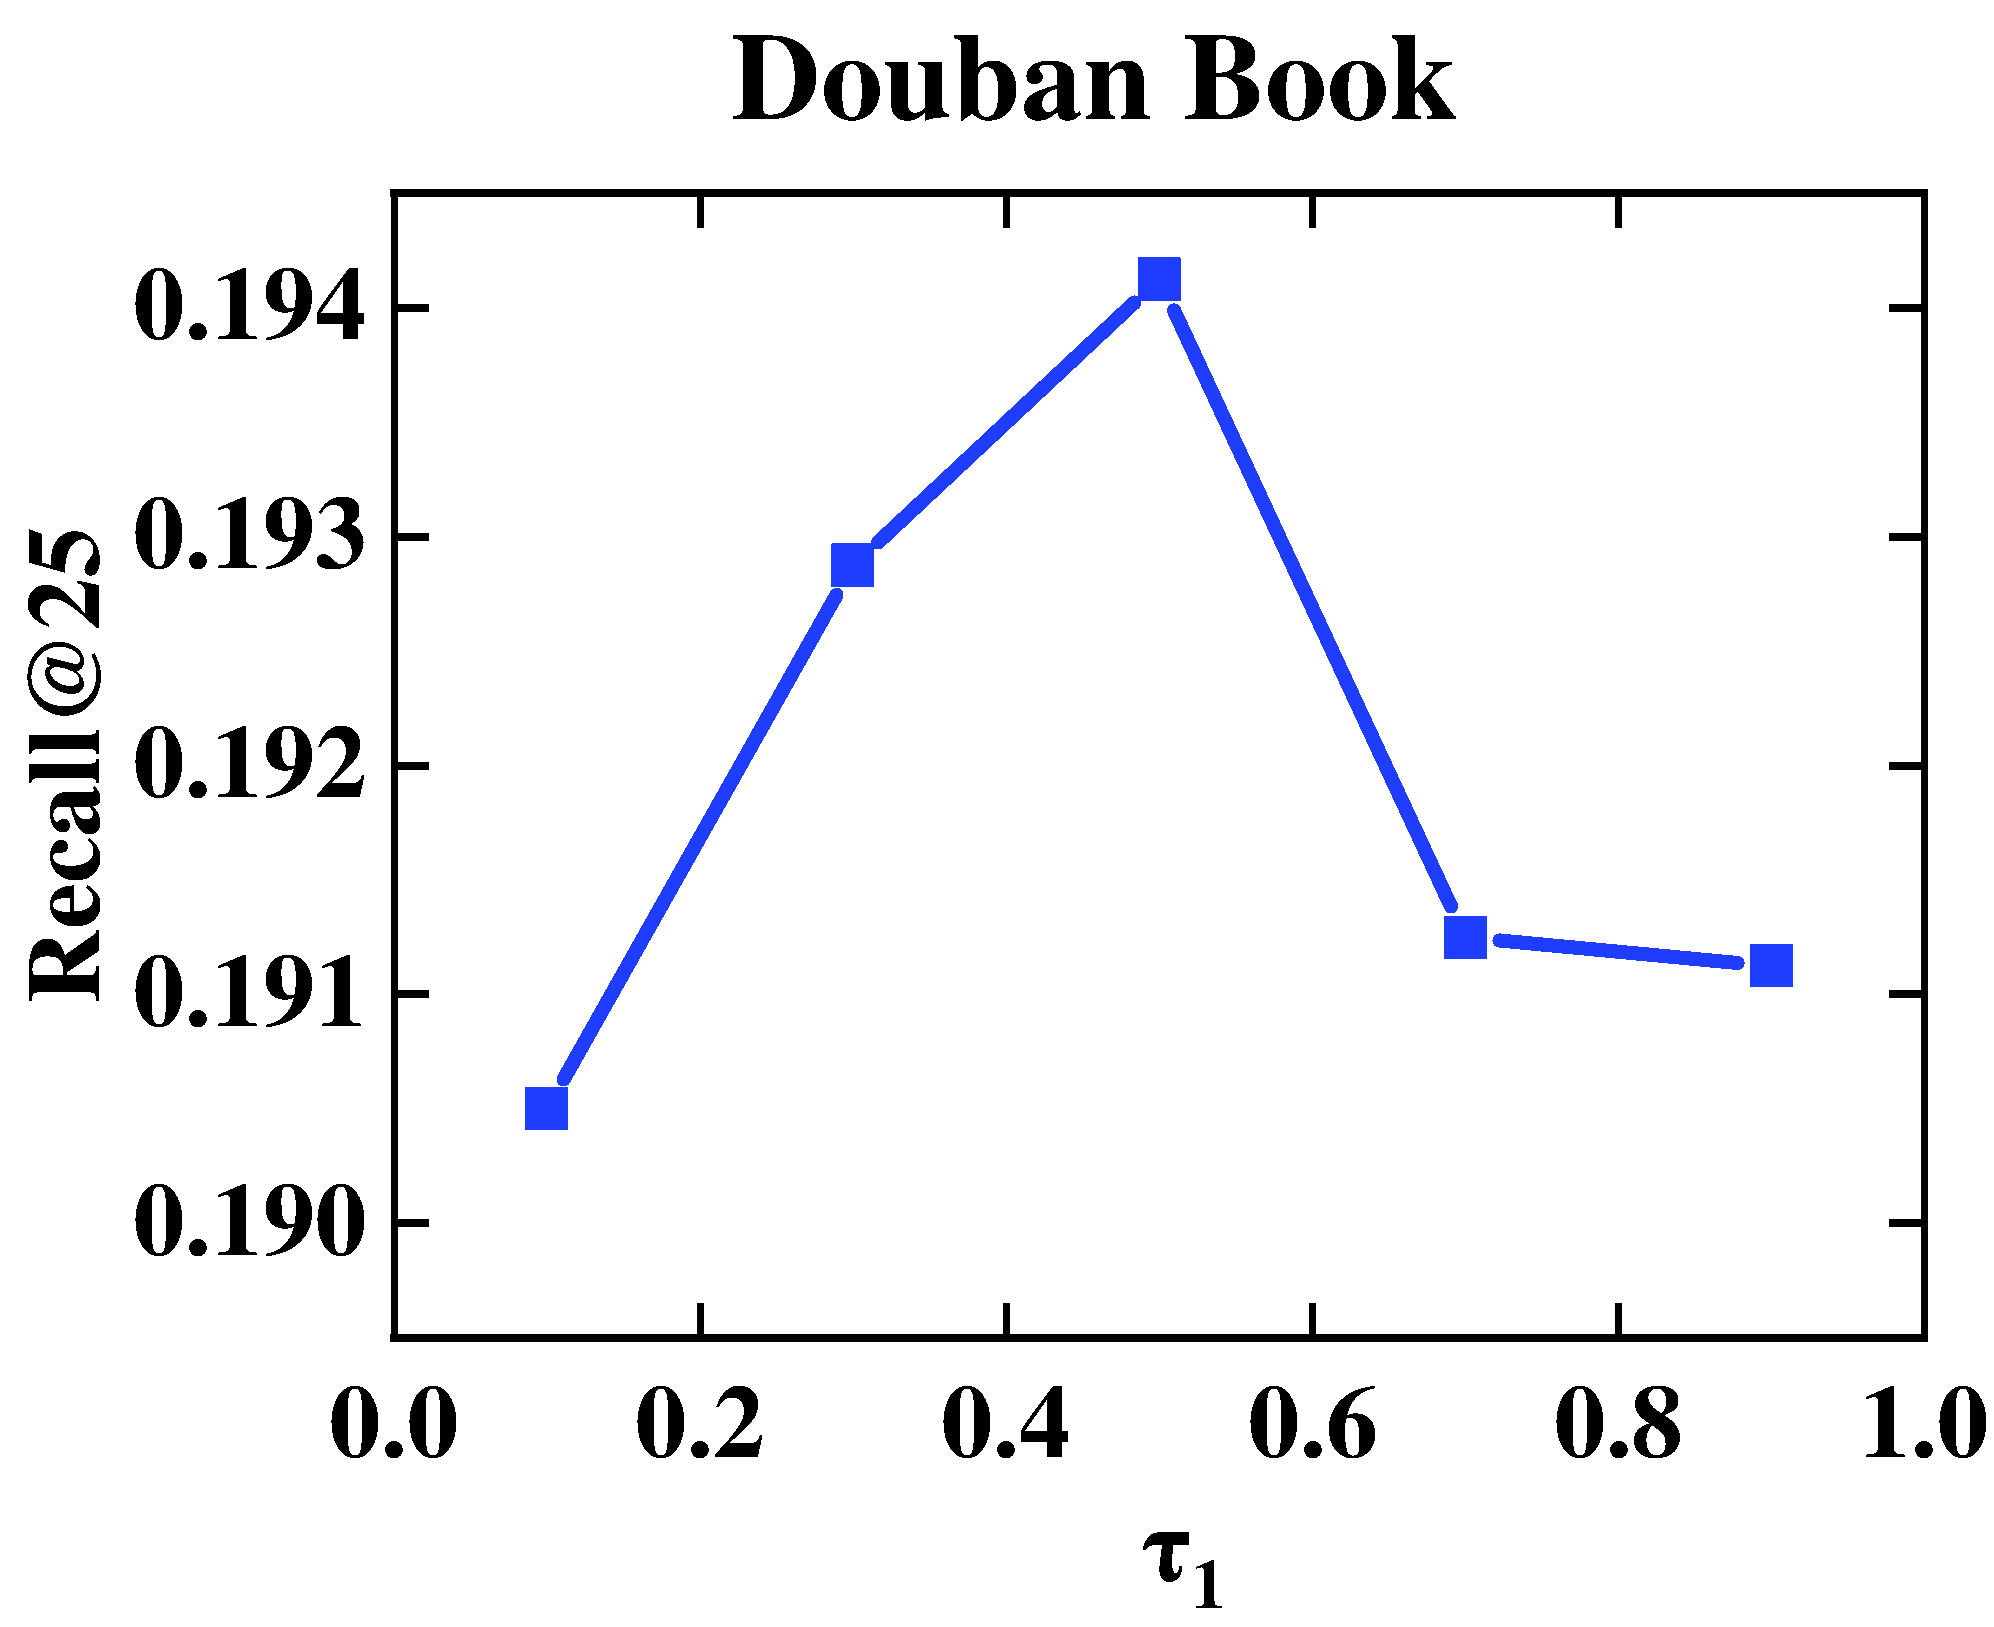
\includegraphics[width=0.25\textwidth]{fig/par/2.pdf}
    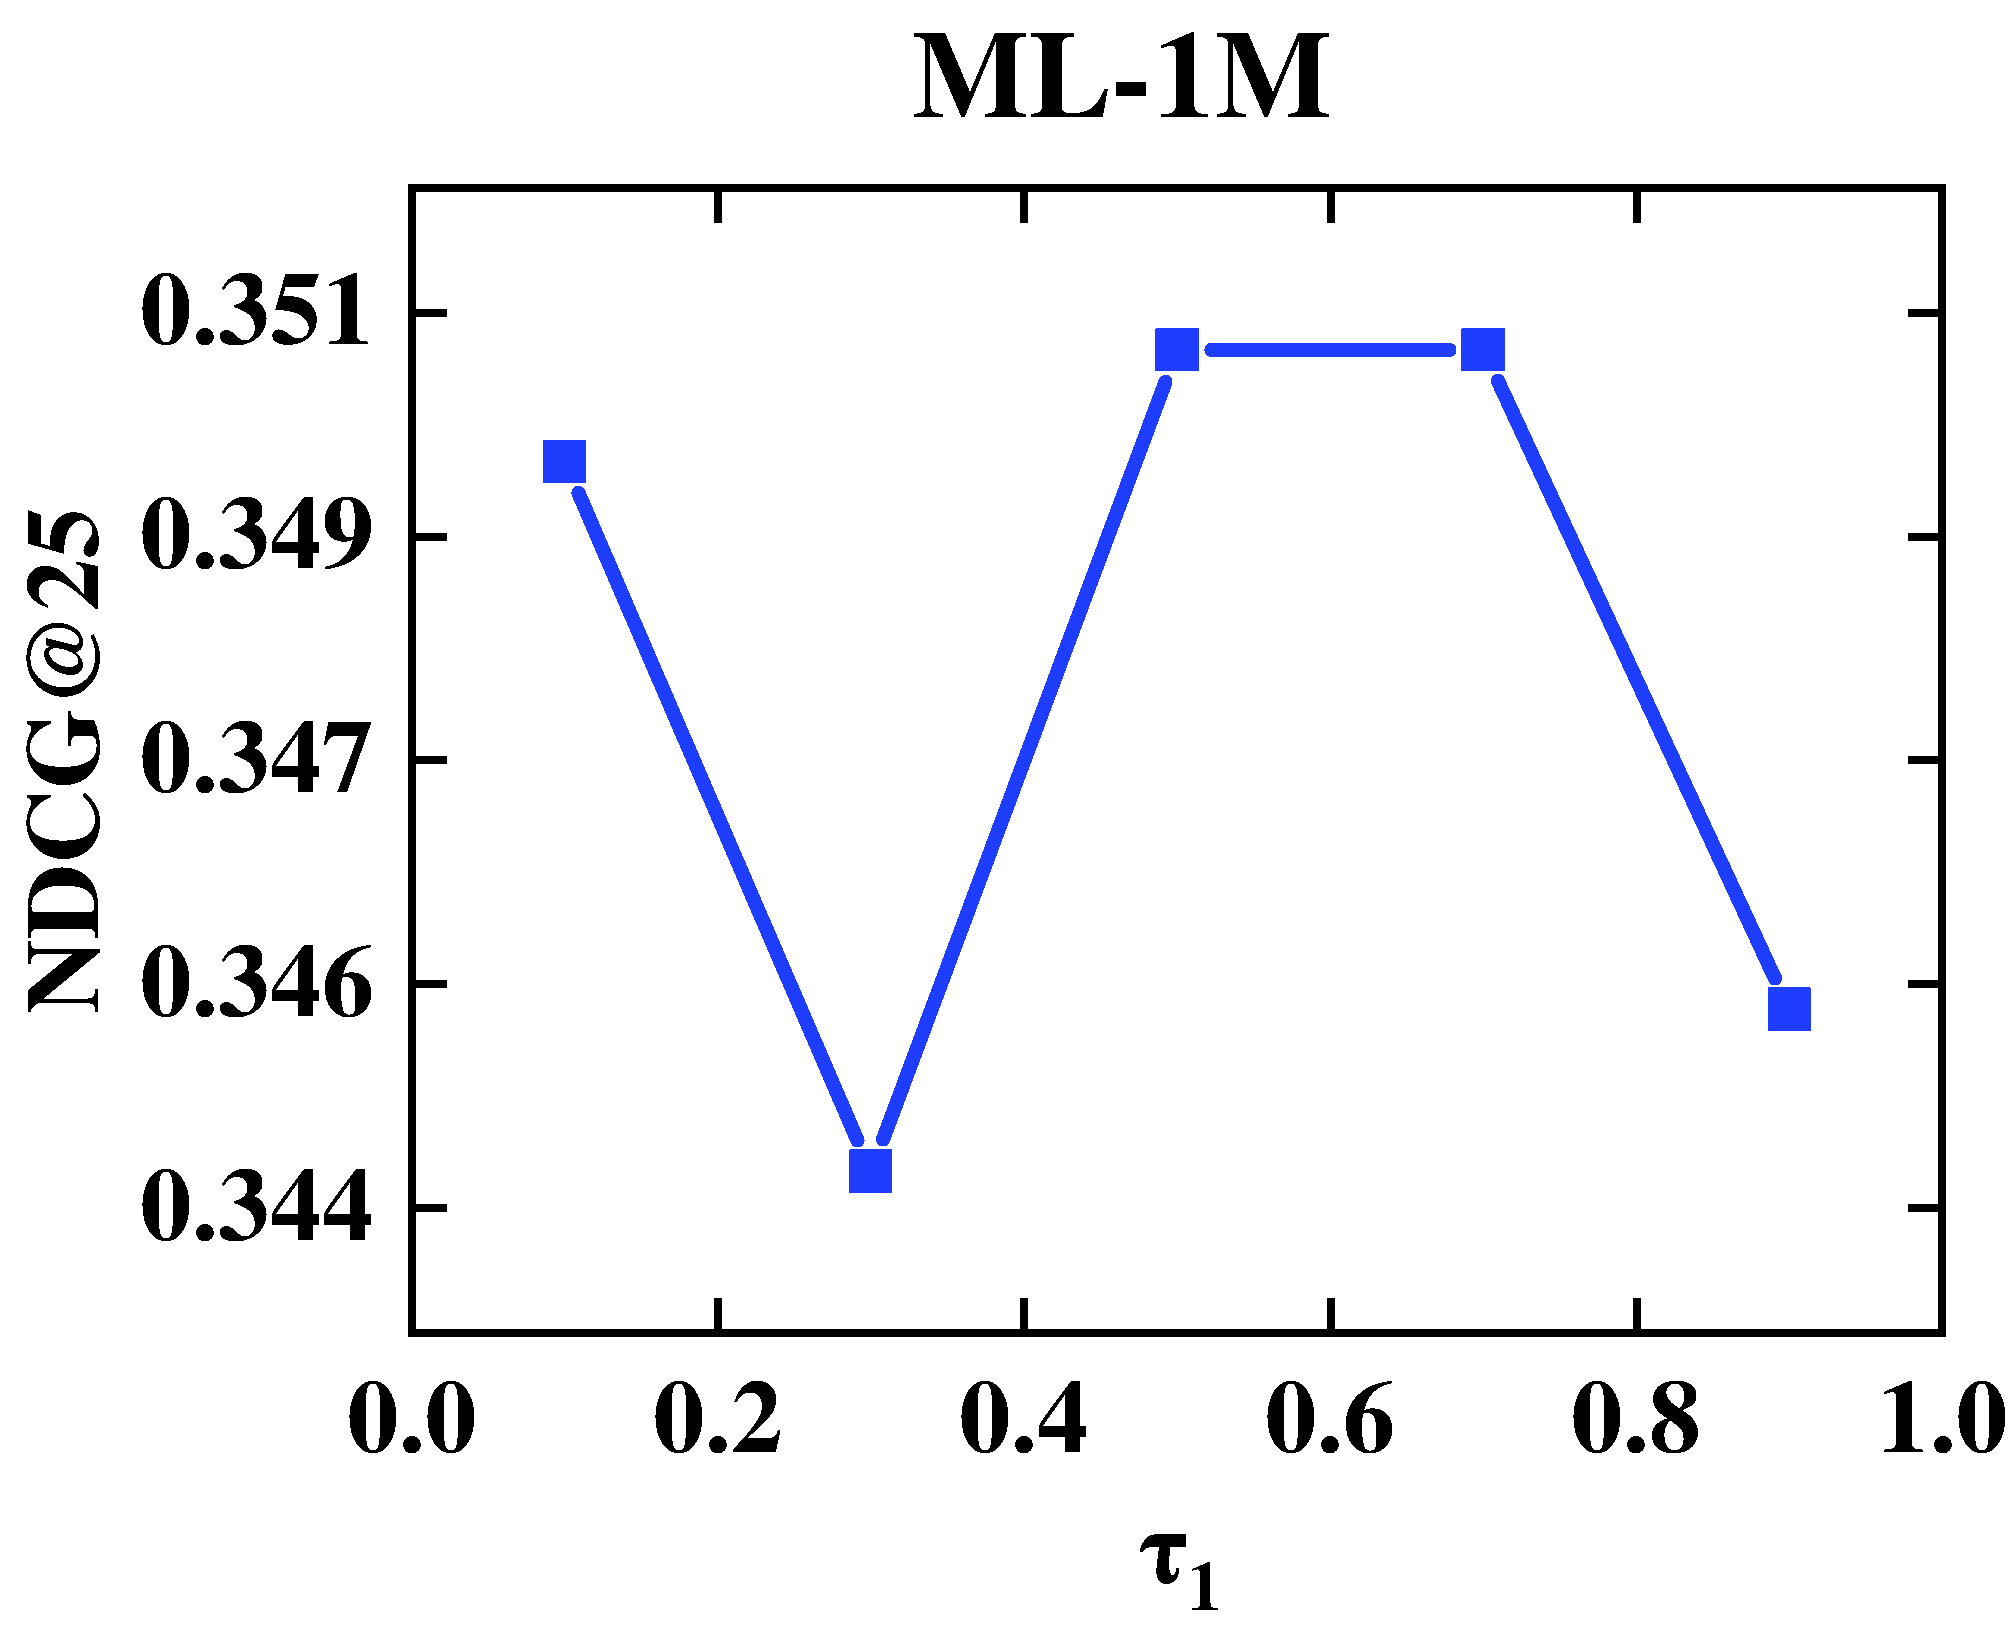
\includegraphics[width=0.25\textwidth]{fig/par/3.pdf}
    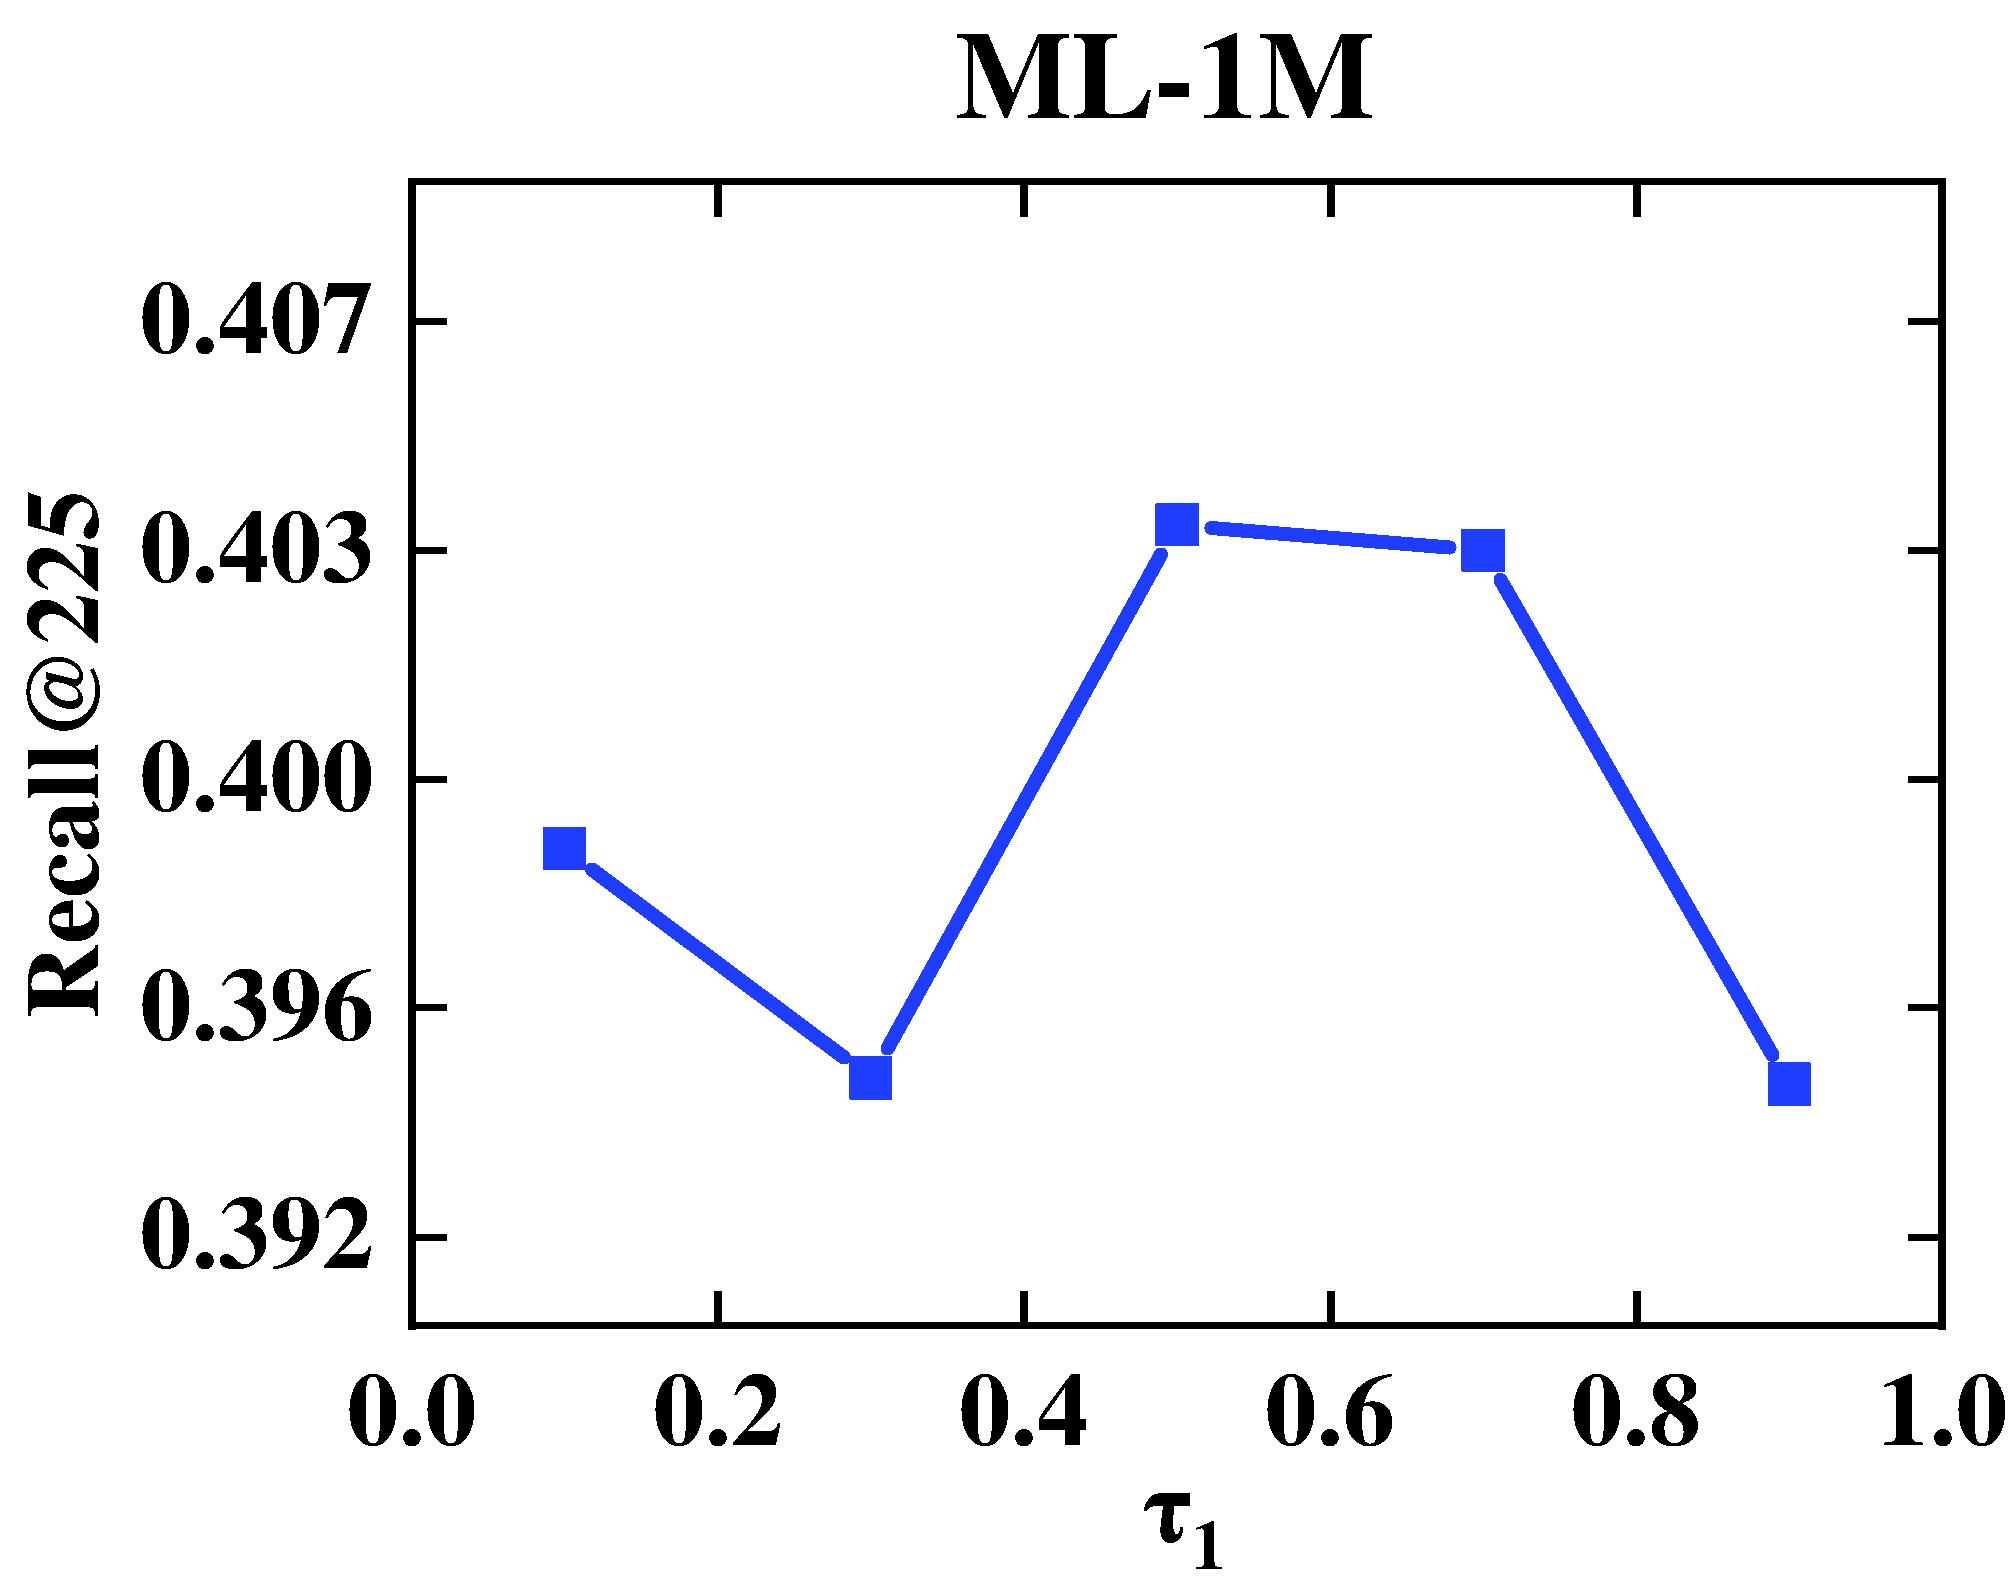
\includegraphics[width=0.25\textwidth]{fig/par/4.pdf}}
\subfigure[Effect of $\tau_2$ (temperature hyper-parameter)]
{\label{tau}
    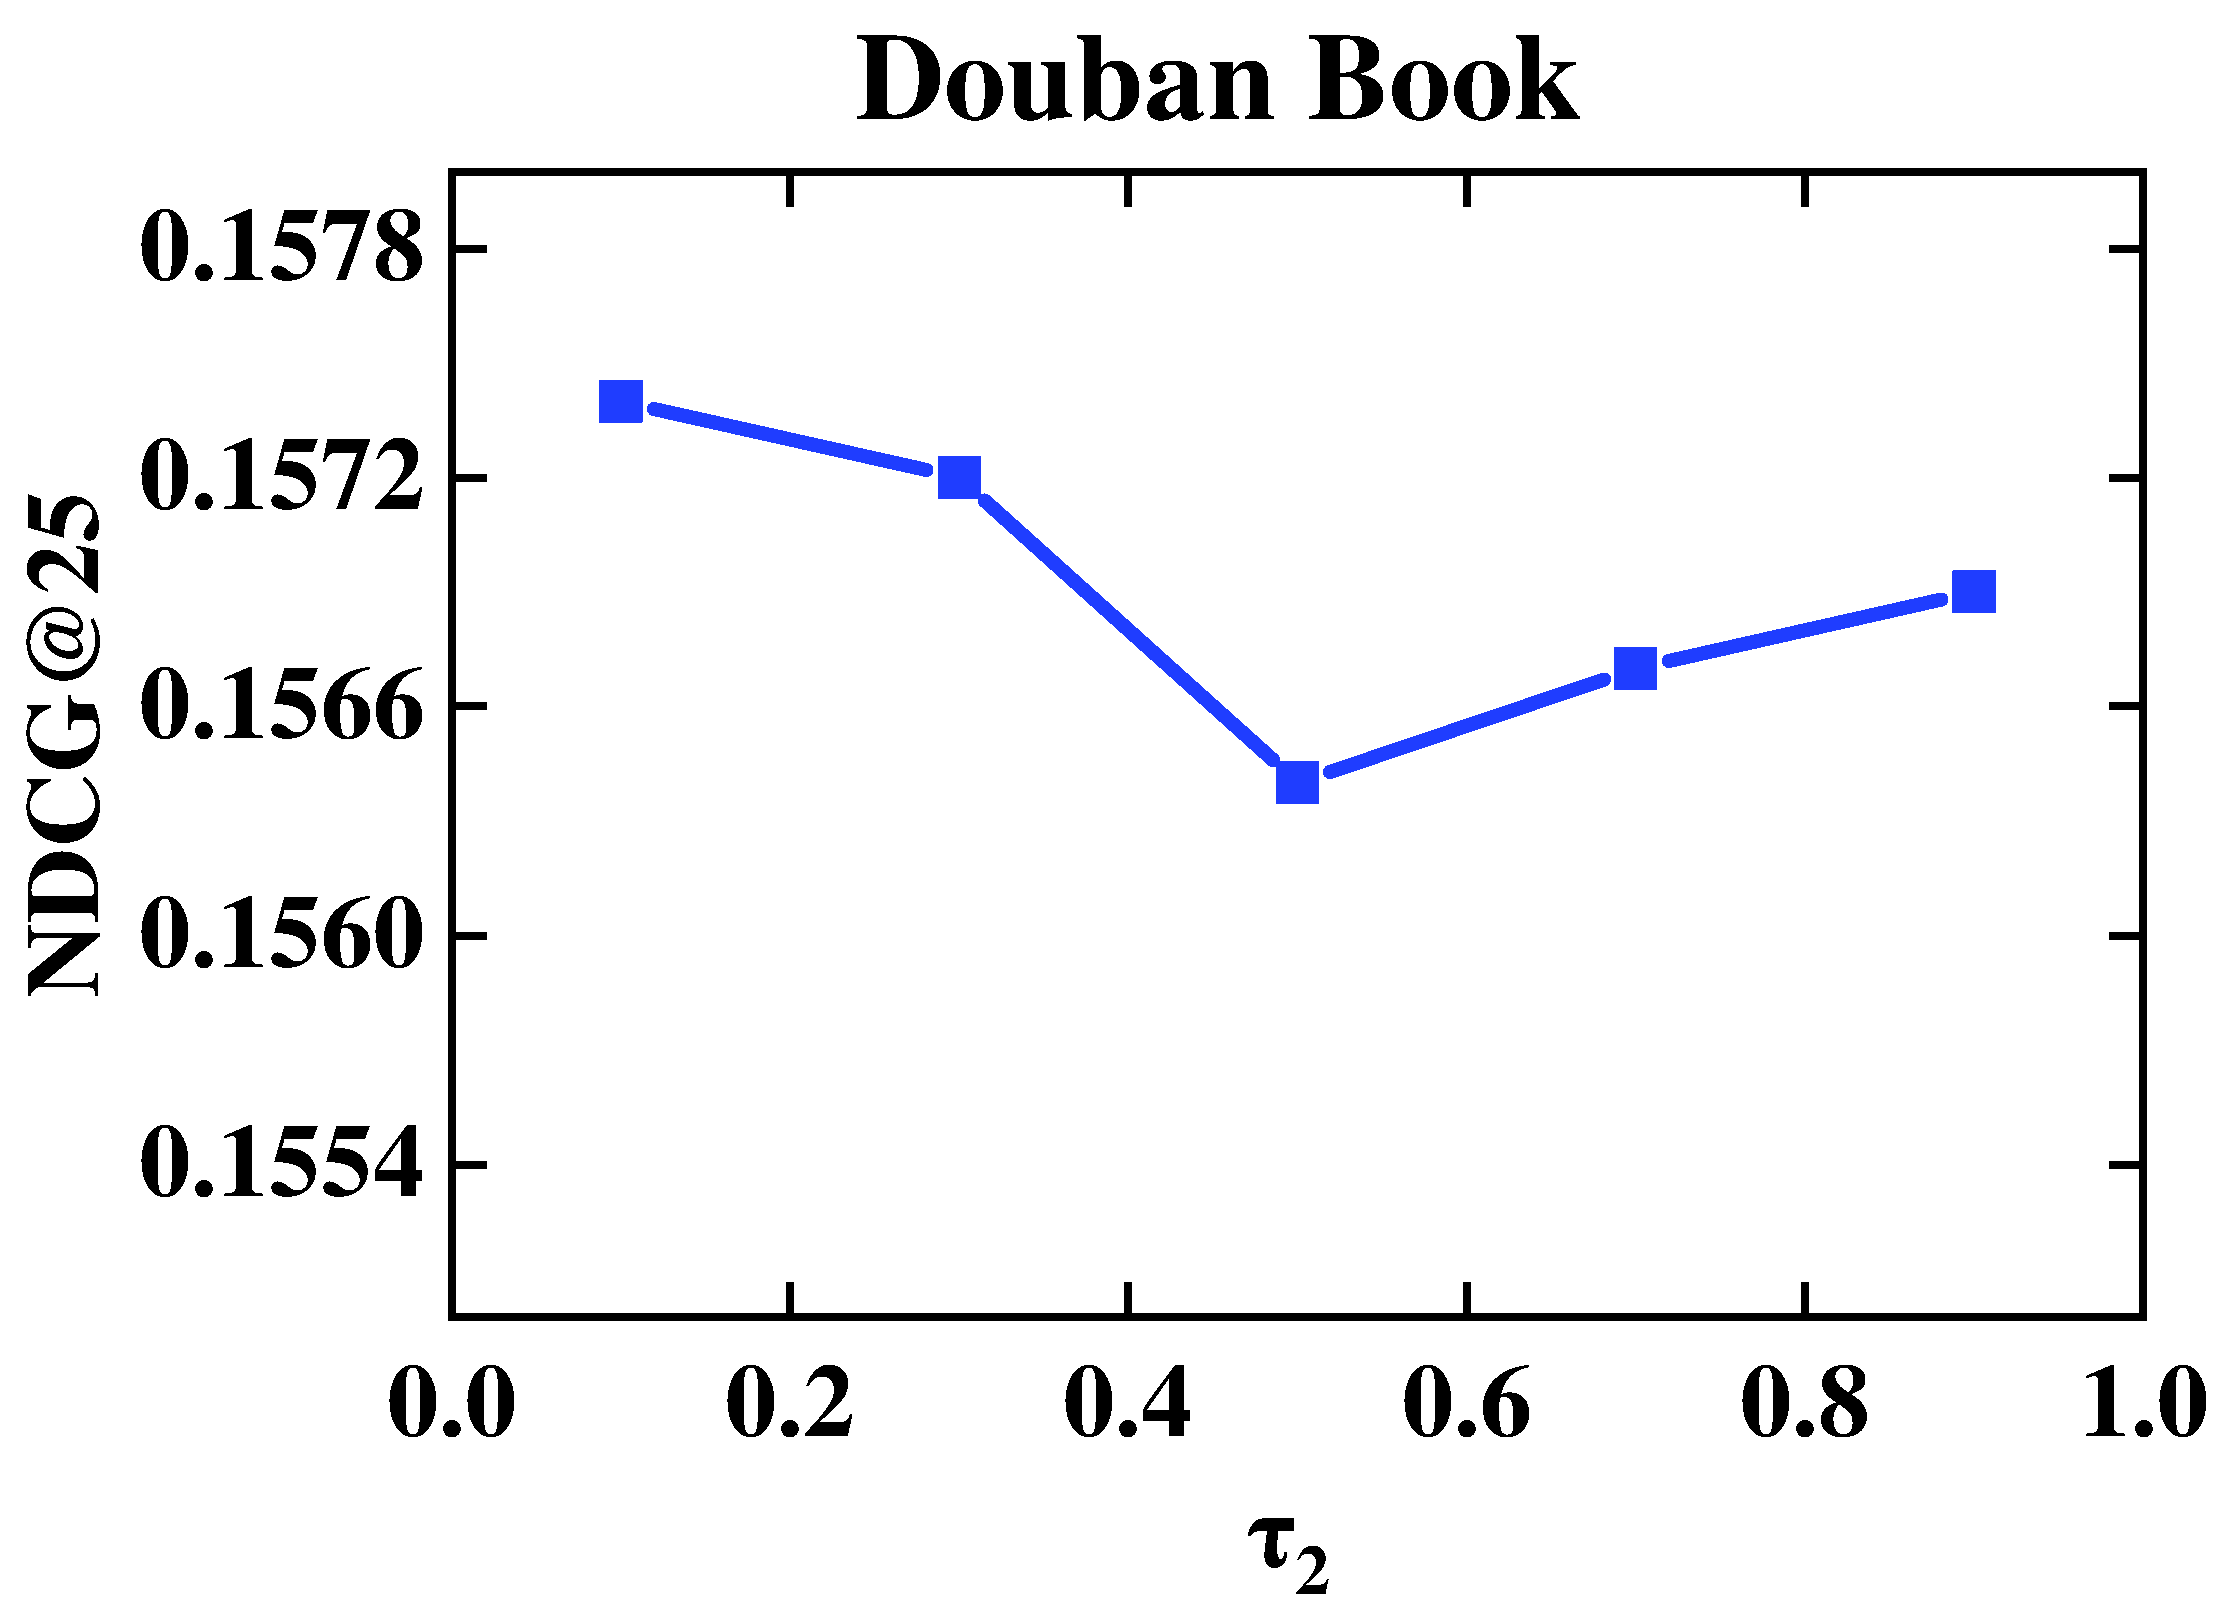
\includegraphics[width=0.25\textwidth]{fig/par/5.pdf}
    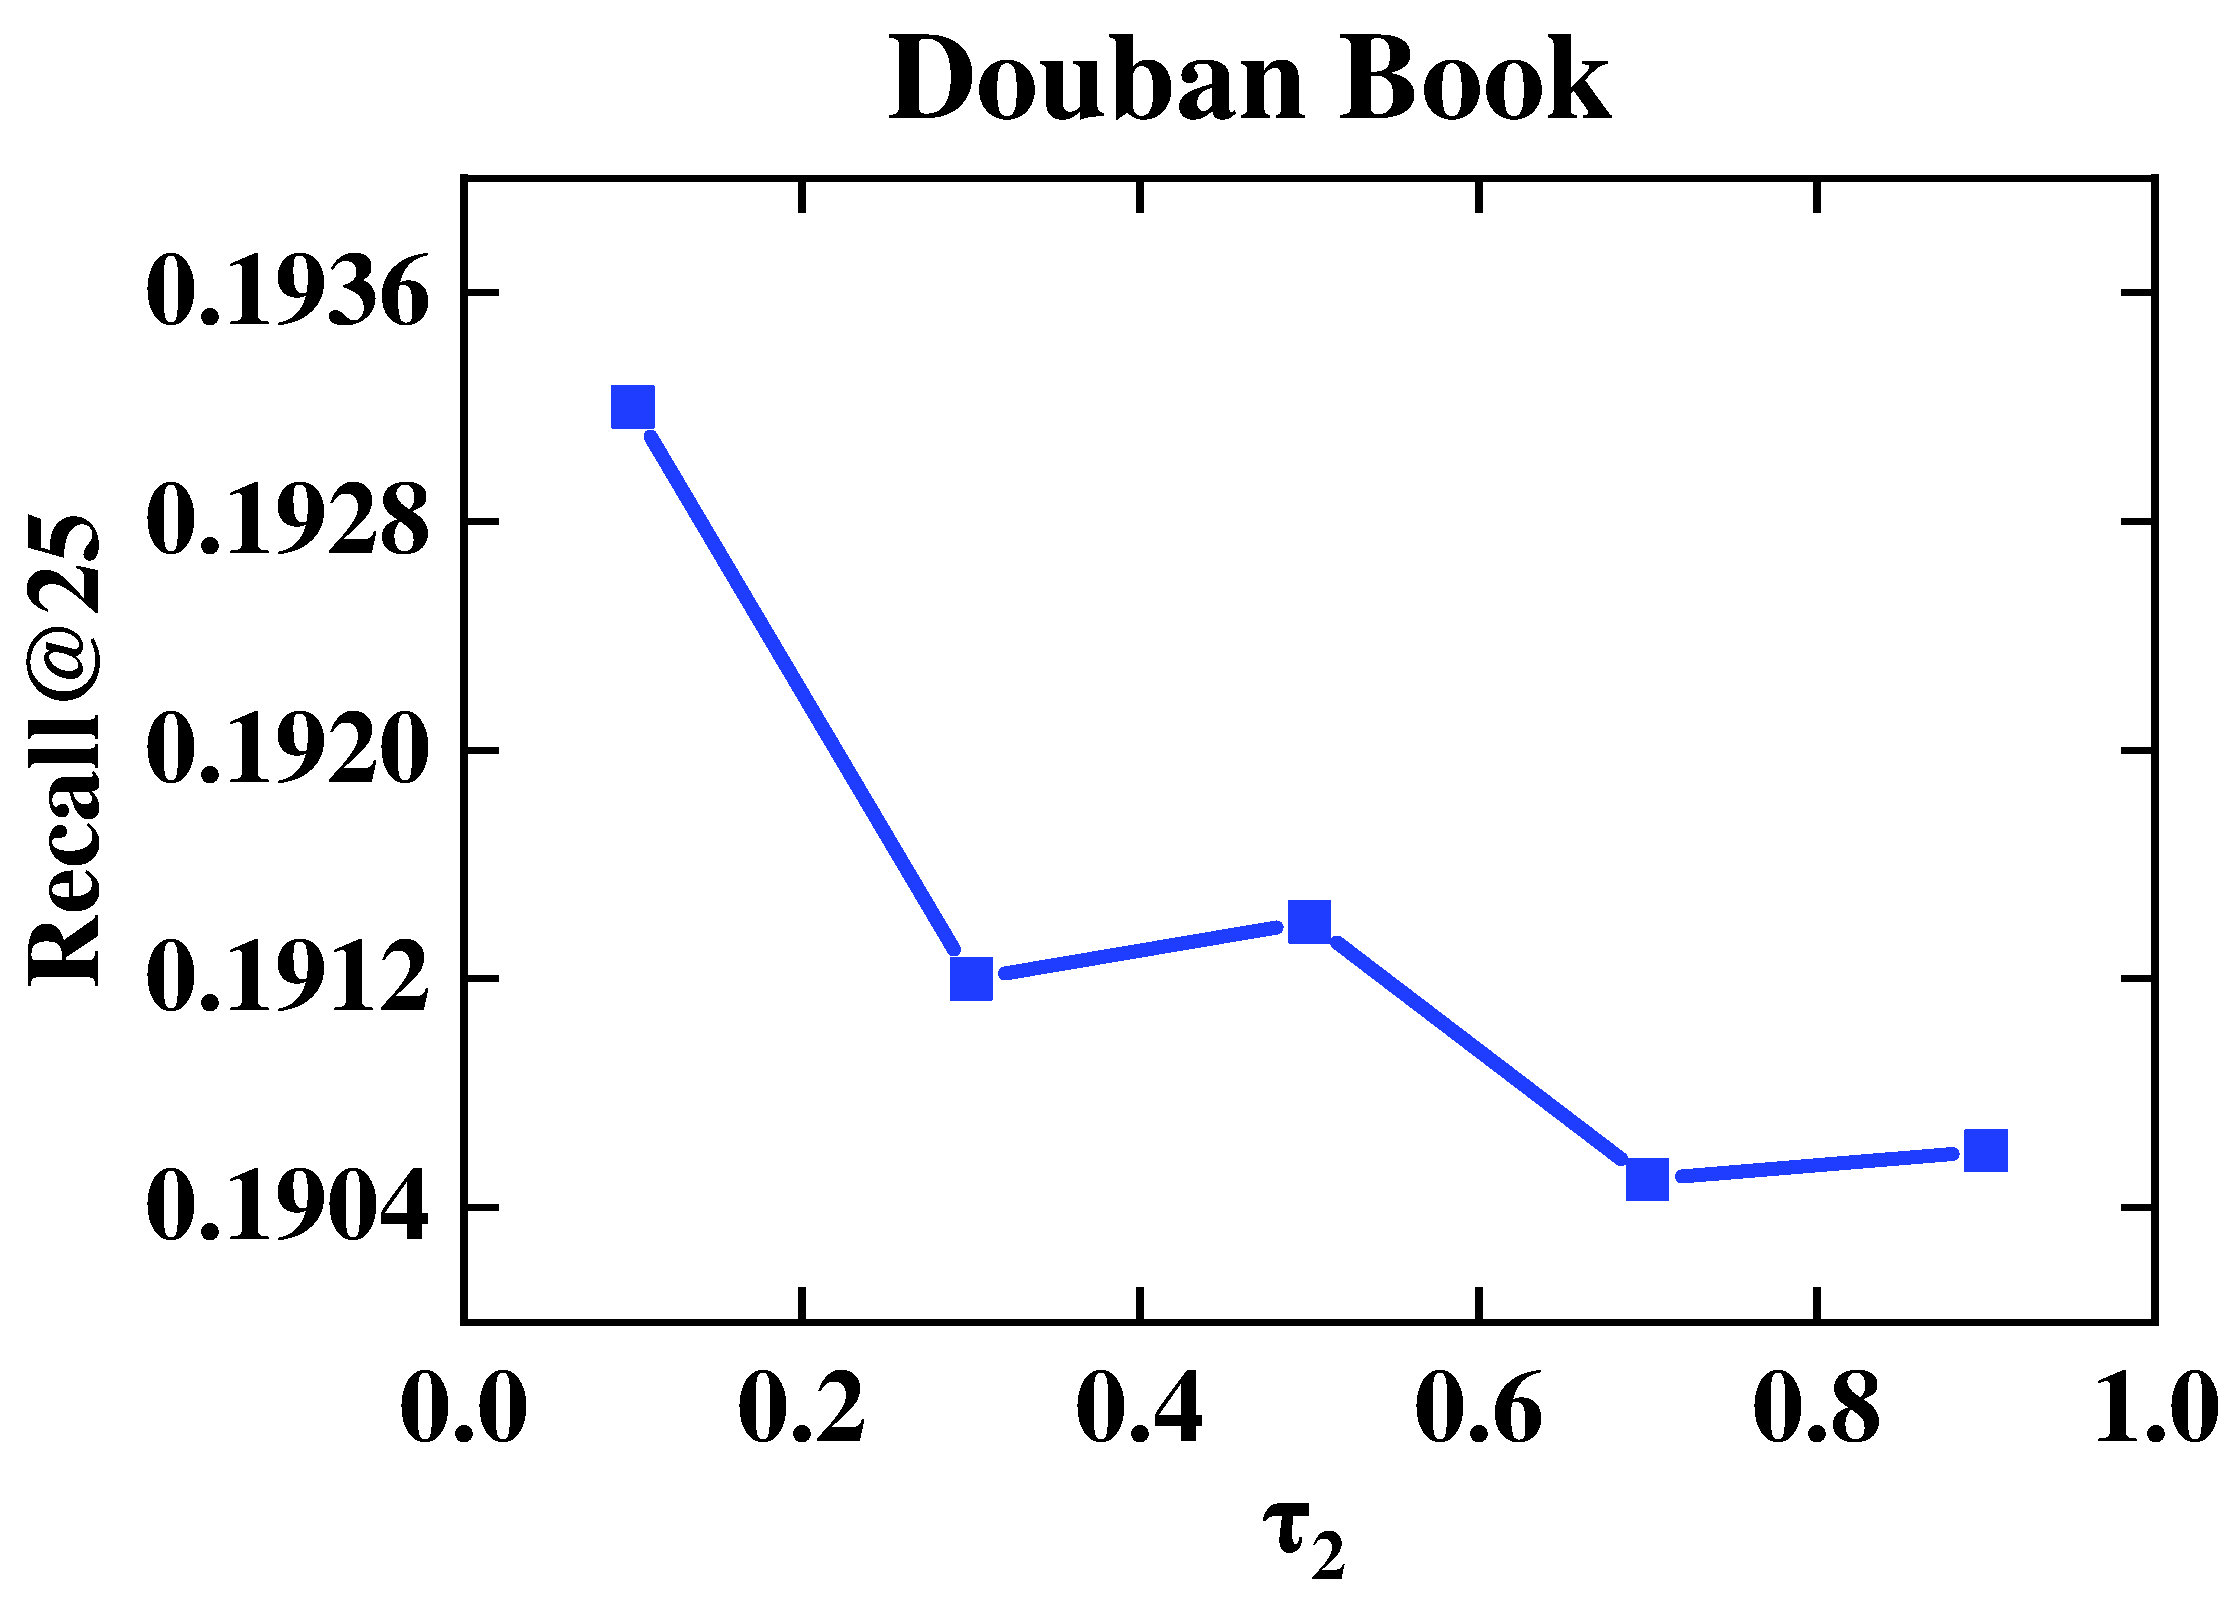
\includegraphics[width=0.25\textwidth]{fig/par/6.pdf}
    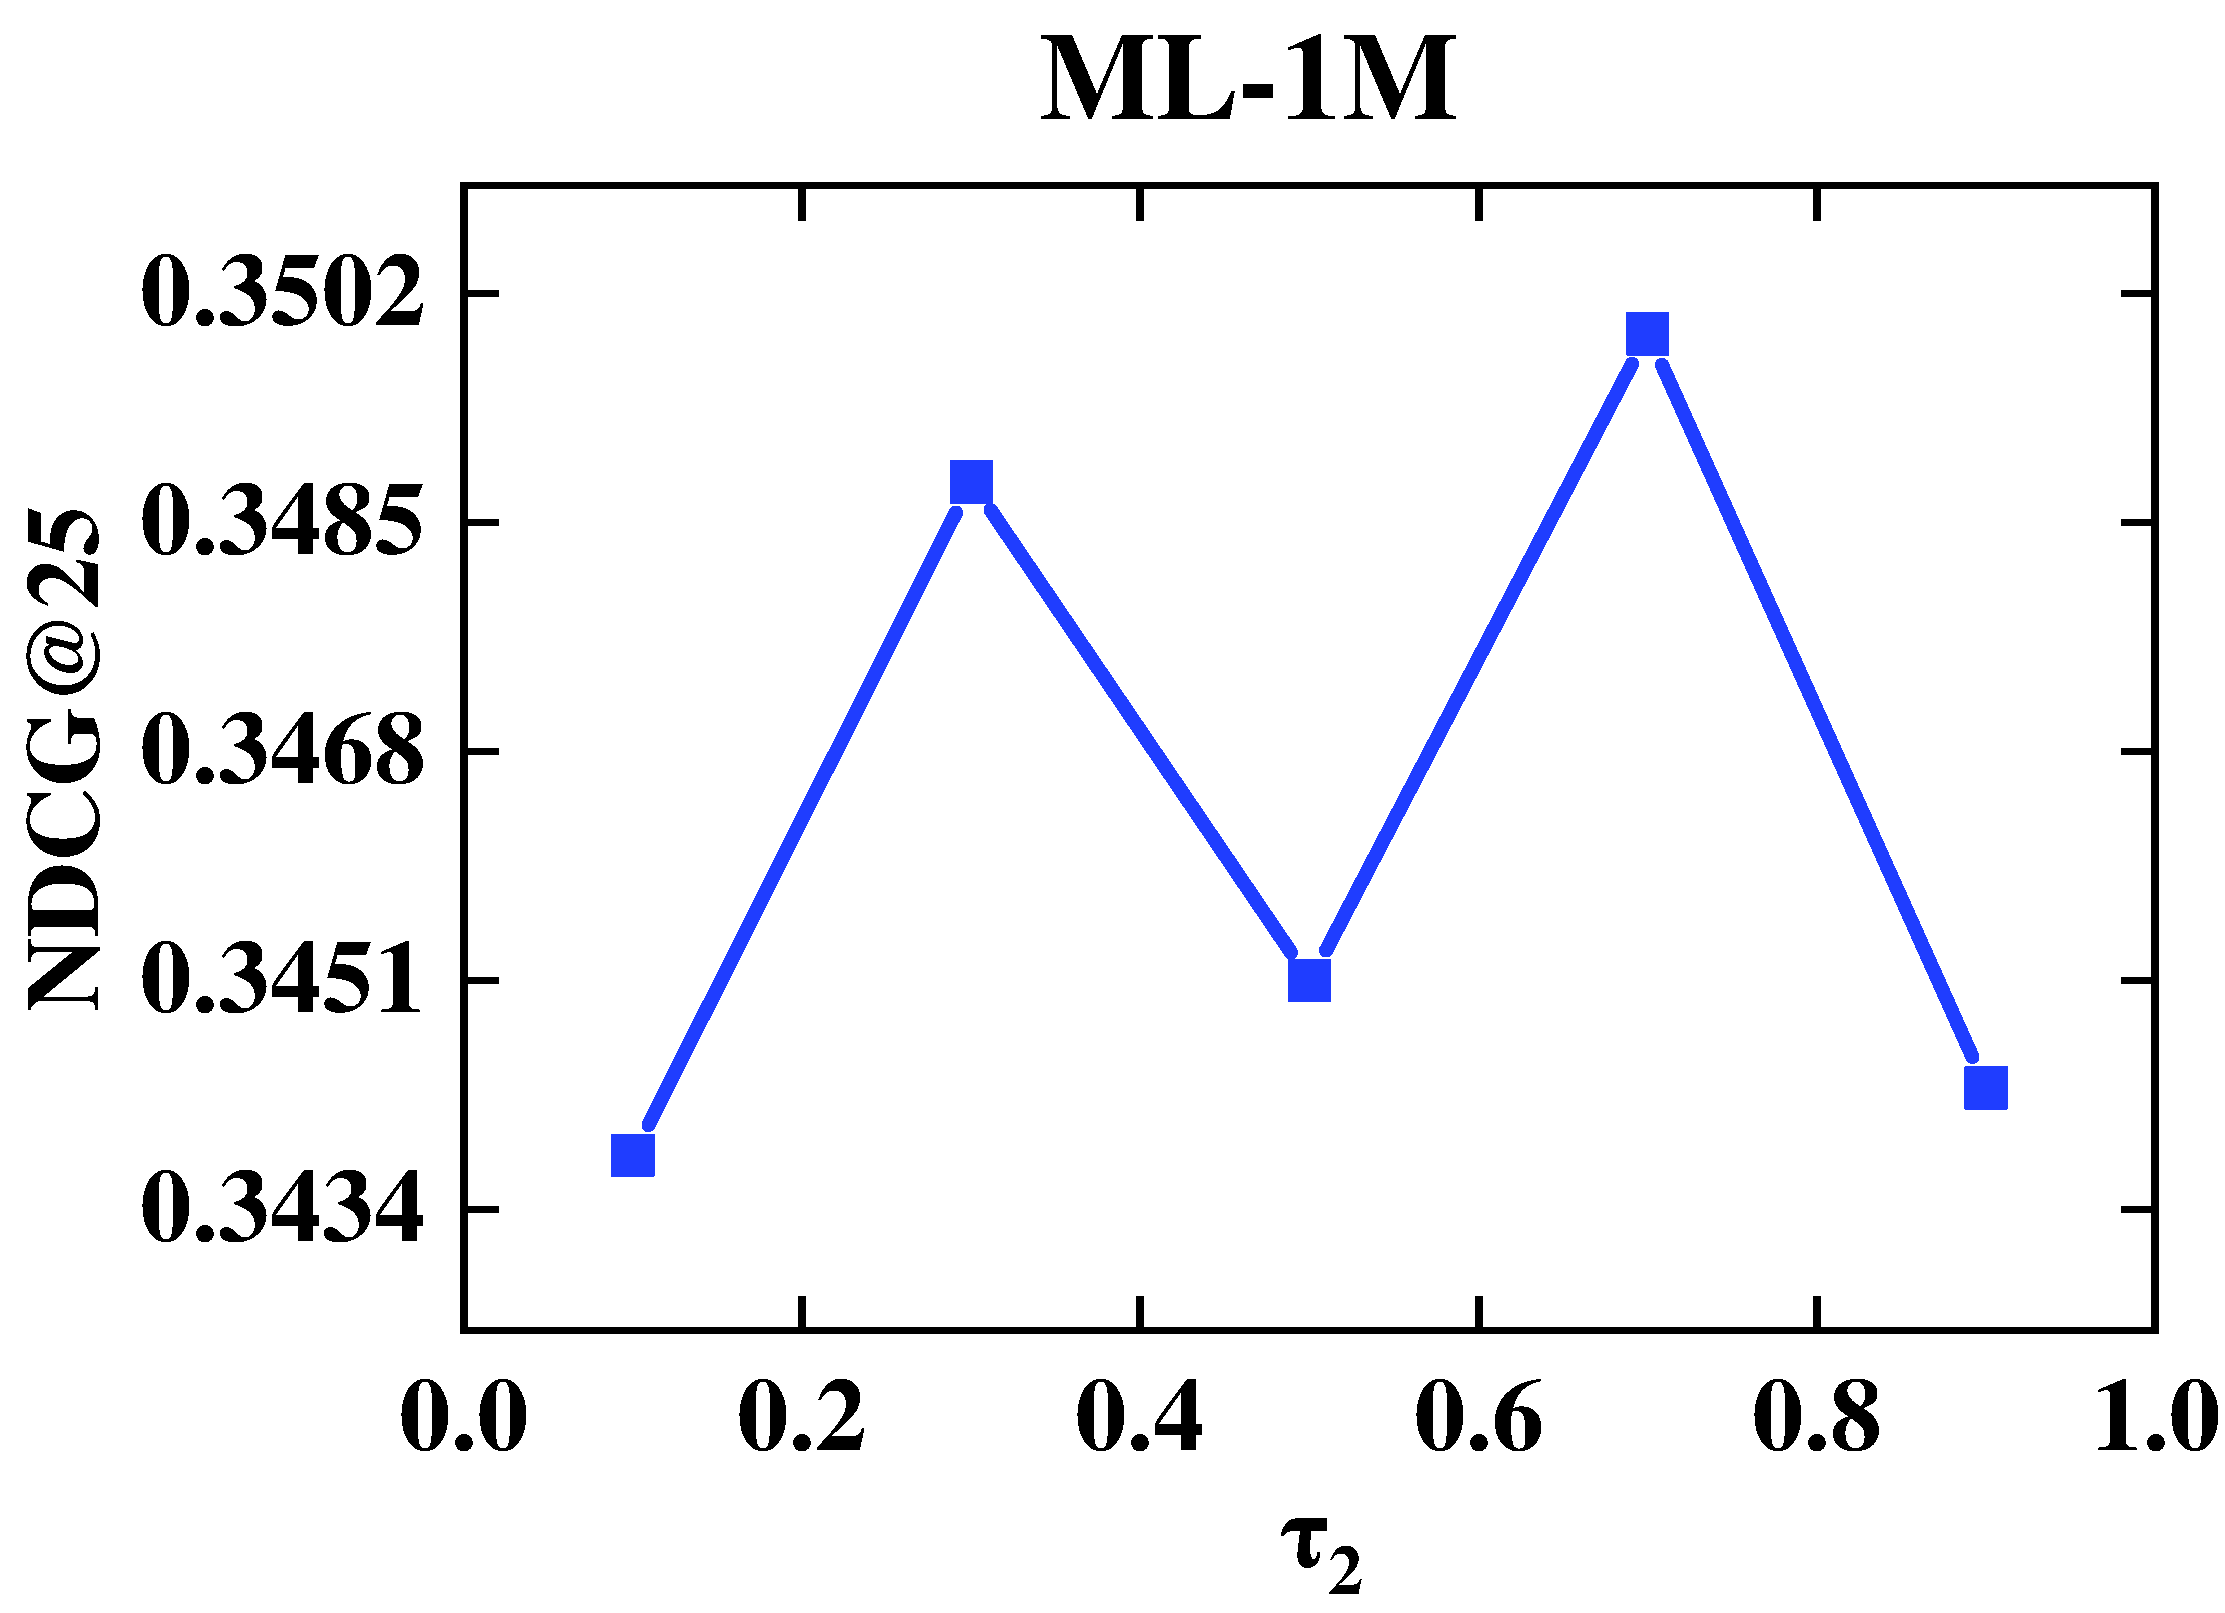
\includegraphics[width=0.25\textwidth]{fig/par/7.pdf}
    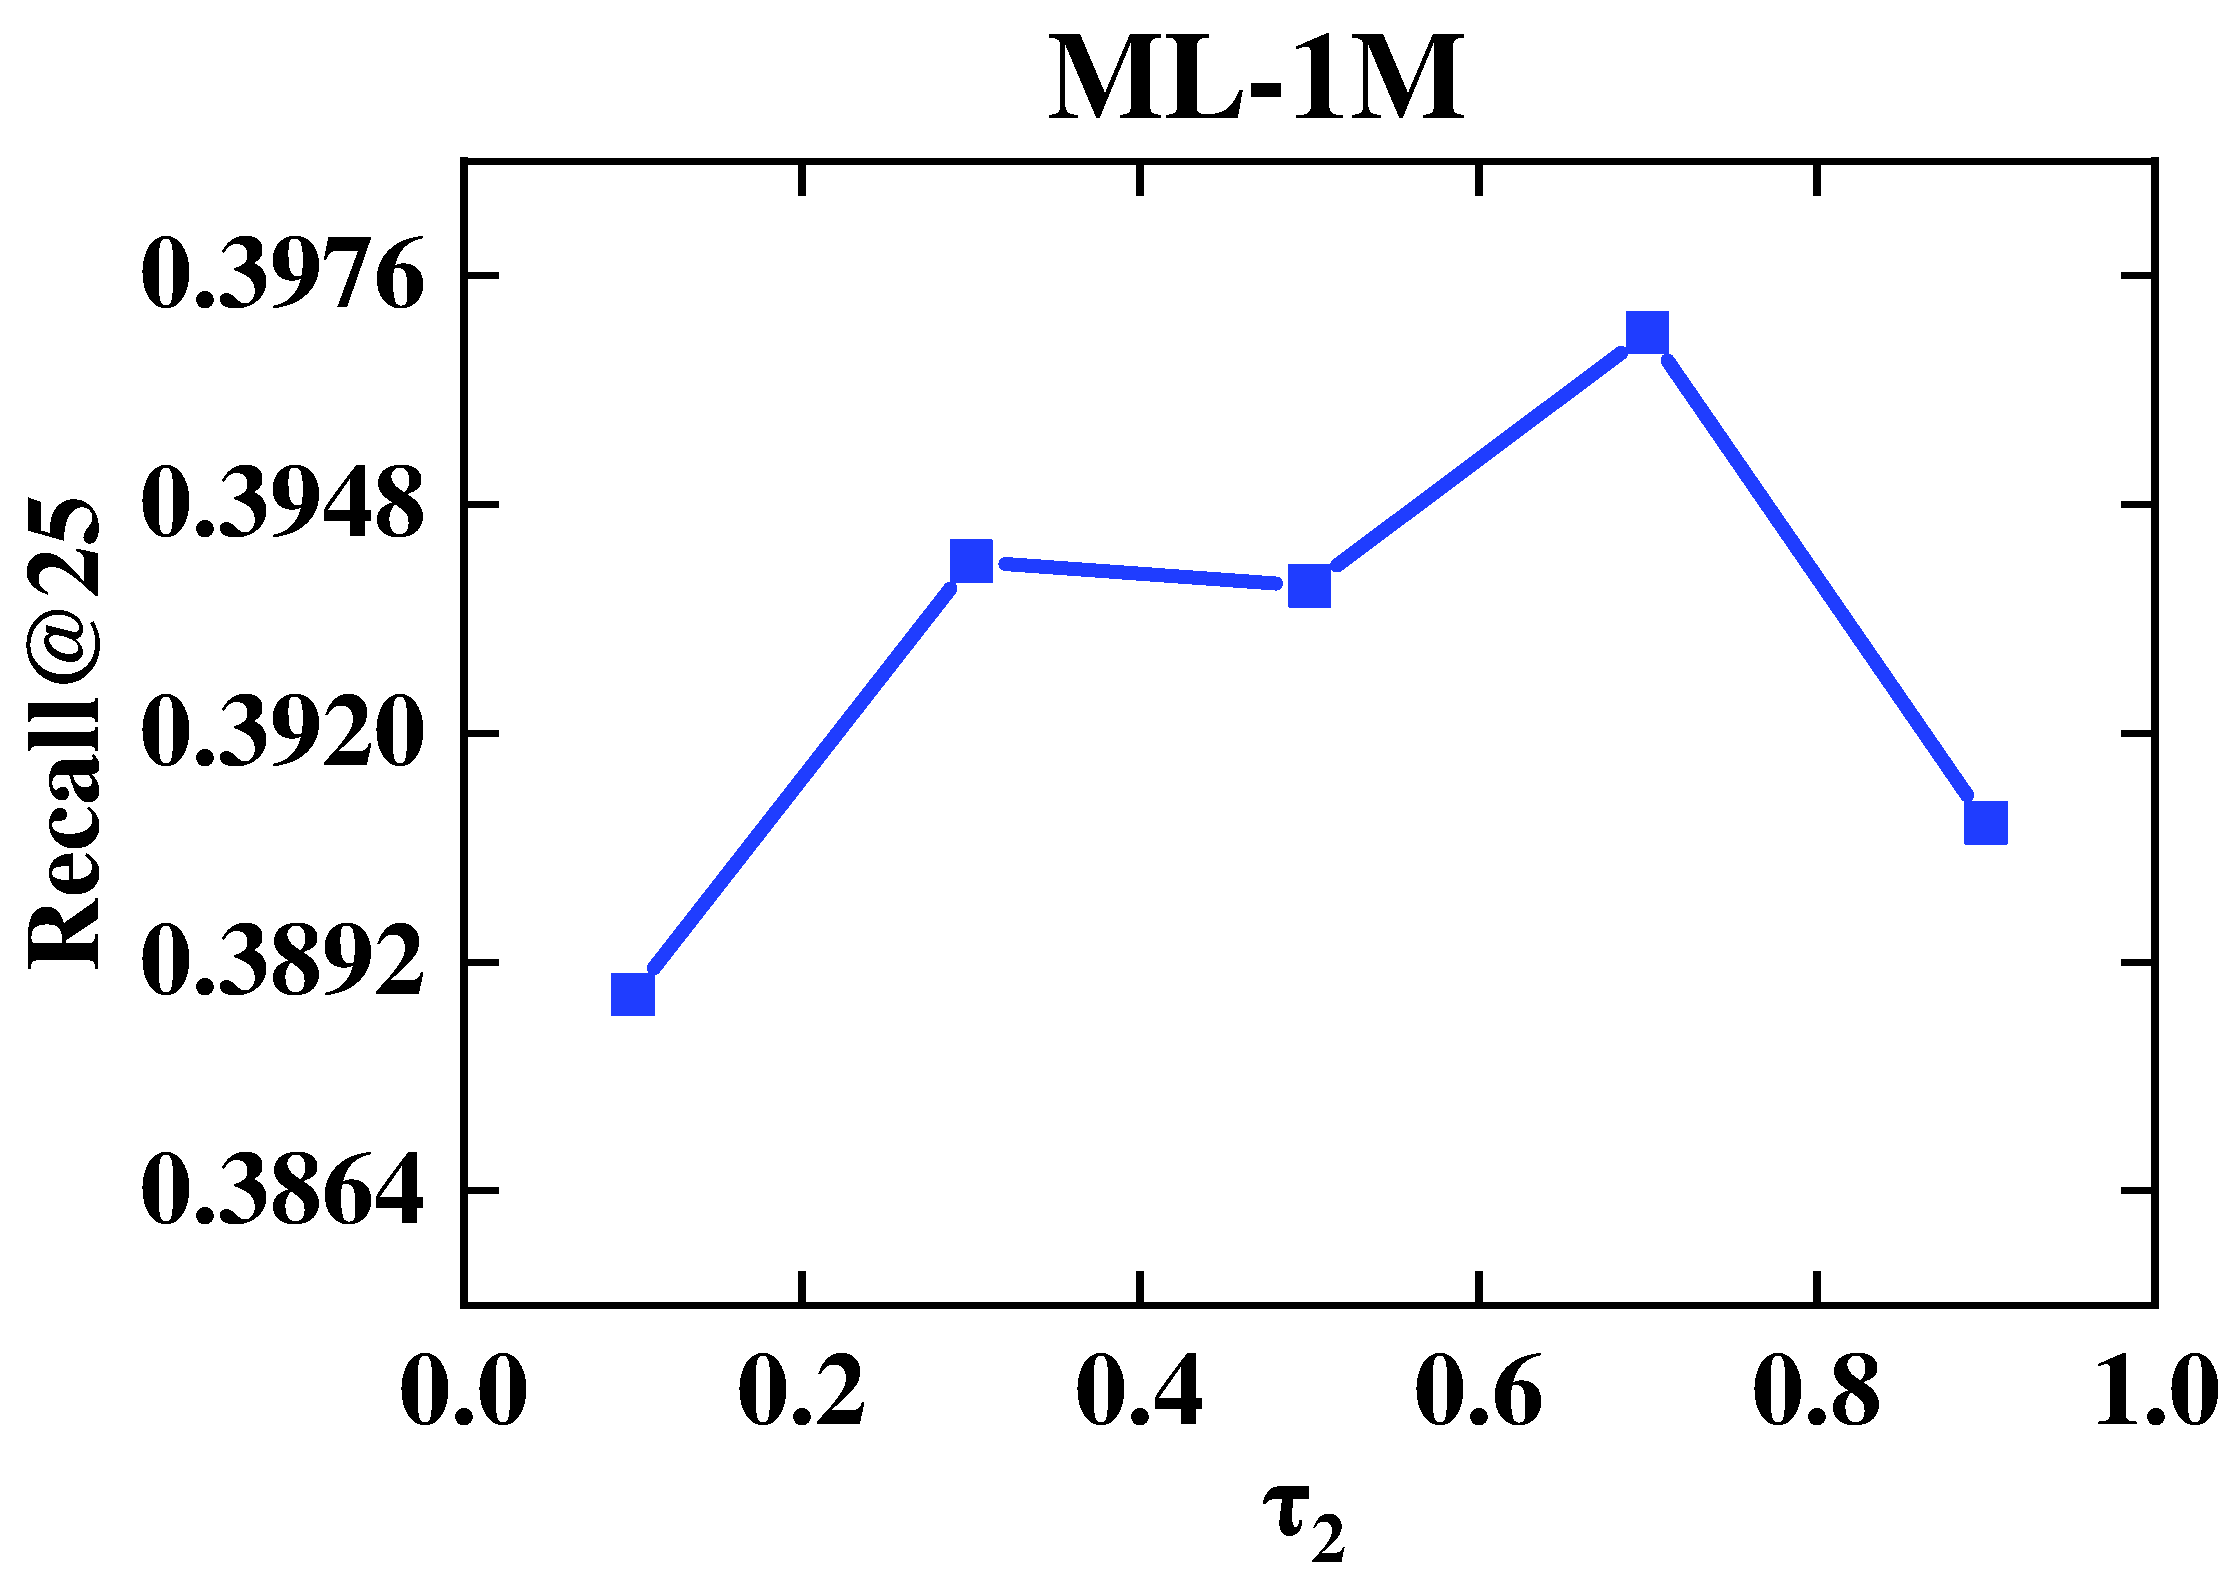
\includegraphics[width=0.25\textwidth]{fig/par/8.pdf}}

\caption{Impact of $\tau_1$ and $\tau_2$ on ML-1M, Douban Book } \label{tau}
\end{figure*}

\begin{table}[]
\begin{center}
    \caption{The Optimal Value of $\tau_1$, $\tau_2$, $\alpha$, $\mathbf{N}_i$ for DSVAE}\label{tab5}
\begin{tabular}{cccc}
\hline \hline
\textbf{Parameters} & \textbf{ML-1M} & \textbf{Douban Book} & \textbf{Epinions} \\ \hline
$\tau_1$ & 0.5 & 0.5 & 0.05   \\
$\tau_2$ & 0.2 & 0.2 & 0.03 \\
$\alpha$  & 0.5 & 0.5 & 0.5    \\
$\mathbf{N}_i$   & 80  & 128 & 150 \\ \hline \hline
\end{tabular}
\end{center}
\end{table}

\subsection{Impact of Hyper-parameters}\label{45}
Furthermore, we study the performance of our proposed method given different parameter settings. The parameter includes $\tau$ (temperature parameter in contrastive loss), $\alpha$ (dropout ratio in data augmentation), $\mathbf{N}_i$ (the number of negative samples). Fig. \ref{tau}, Fig. \ref{alpha} and Fig. \ref{N_u} respectively illustrate how DSVAE performs under different $\tau$, $\alpha$ and $\mathbf{N}_i$ configurations. We study the sensitivity
analysis of DSVAE in the following subsections. Due to the space limitation, we omit the results on Epinions which have a similar trend to that on ML-1M and Douban Book. And the empirically optimal values of these hyper-parameters are shown in Table \ref{tab5}.


\subsubsection{Effect of SSL weight $\tau$}\label{subsubsec2}
The temperature parameter $\tau_1$ and $\tau_2$ control penalties strength on hard negative samples \cite{DBLP:journals/corr/abs-2012-09740}. To investigate the effect of $\tau$ empirically, we conduct the experiments
under different $\tau$ configuration and express the comparing
results in Fig. \ref{tau}.
As described in Fig. \ref{tau}, with the increasing of $\tau_1$ and $\tau_2$, the performance of  DSVAE at first increases and later decreases. And such phenomenon is intuitive, i.e.,
algorithm with smaller $\tau_1$ and $\tau_2$ indicates that too much attention to a few negative samples will loss the supremacy of adding multiple negative samples in the SSL objective; and larger $\tau_1$ and $\tau_2$ will lead model fall short in the ability to discriminate hard negatives samples.

\begin{figure*}[!htb]
\centering
%\subfigure[Effect of $\tau_1$ (temperature hyper-parameter) ]
{\label{lambda}
    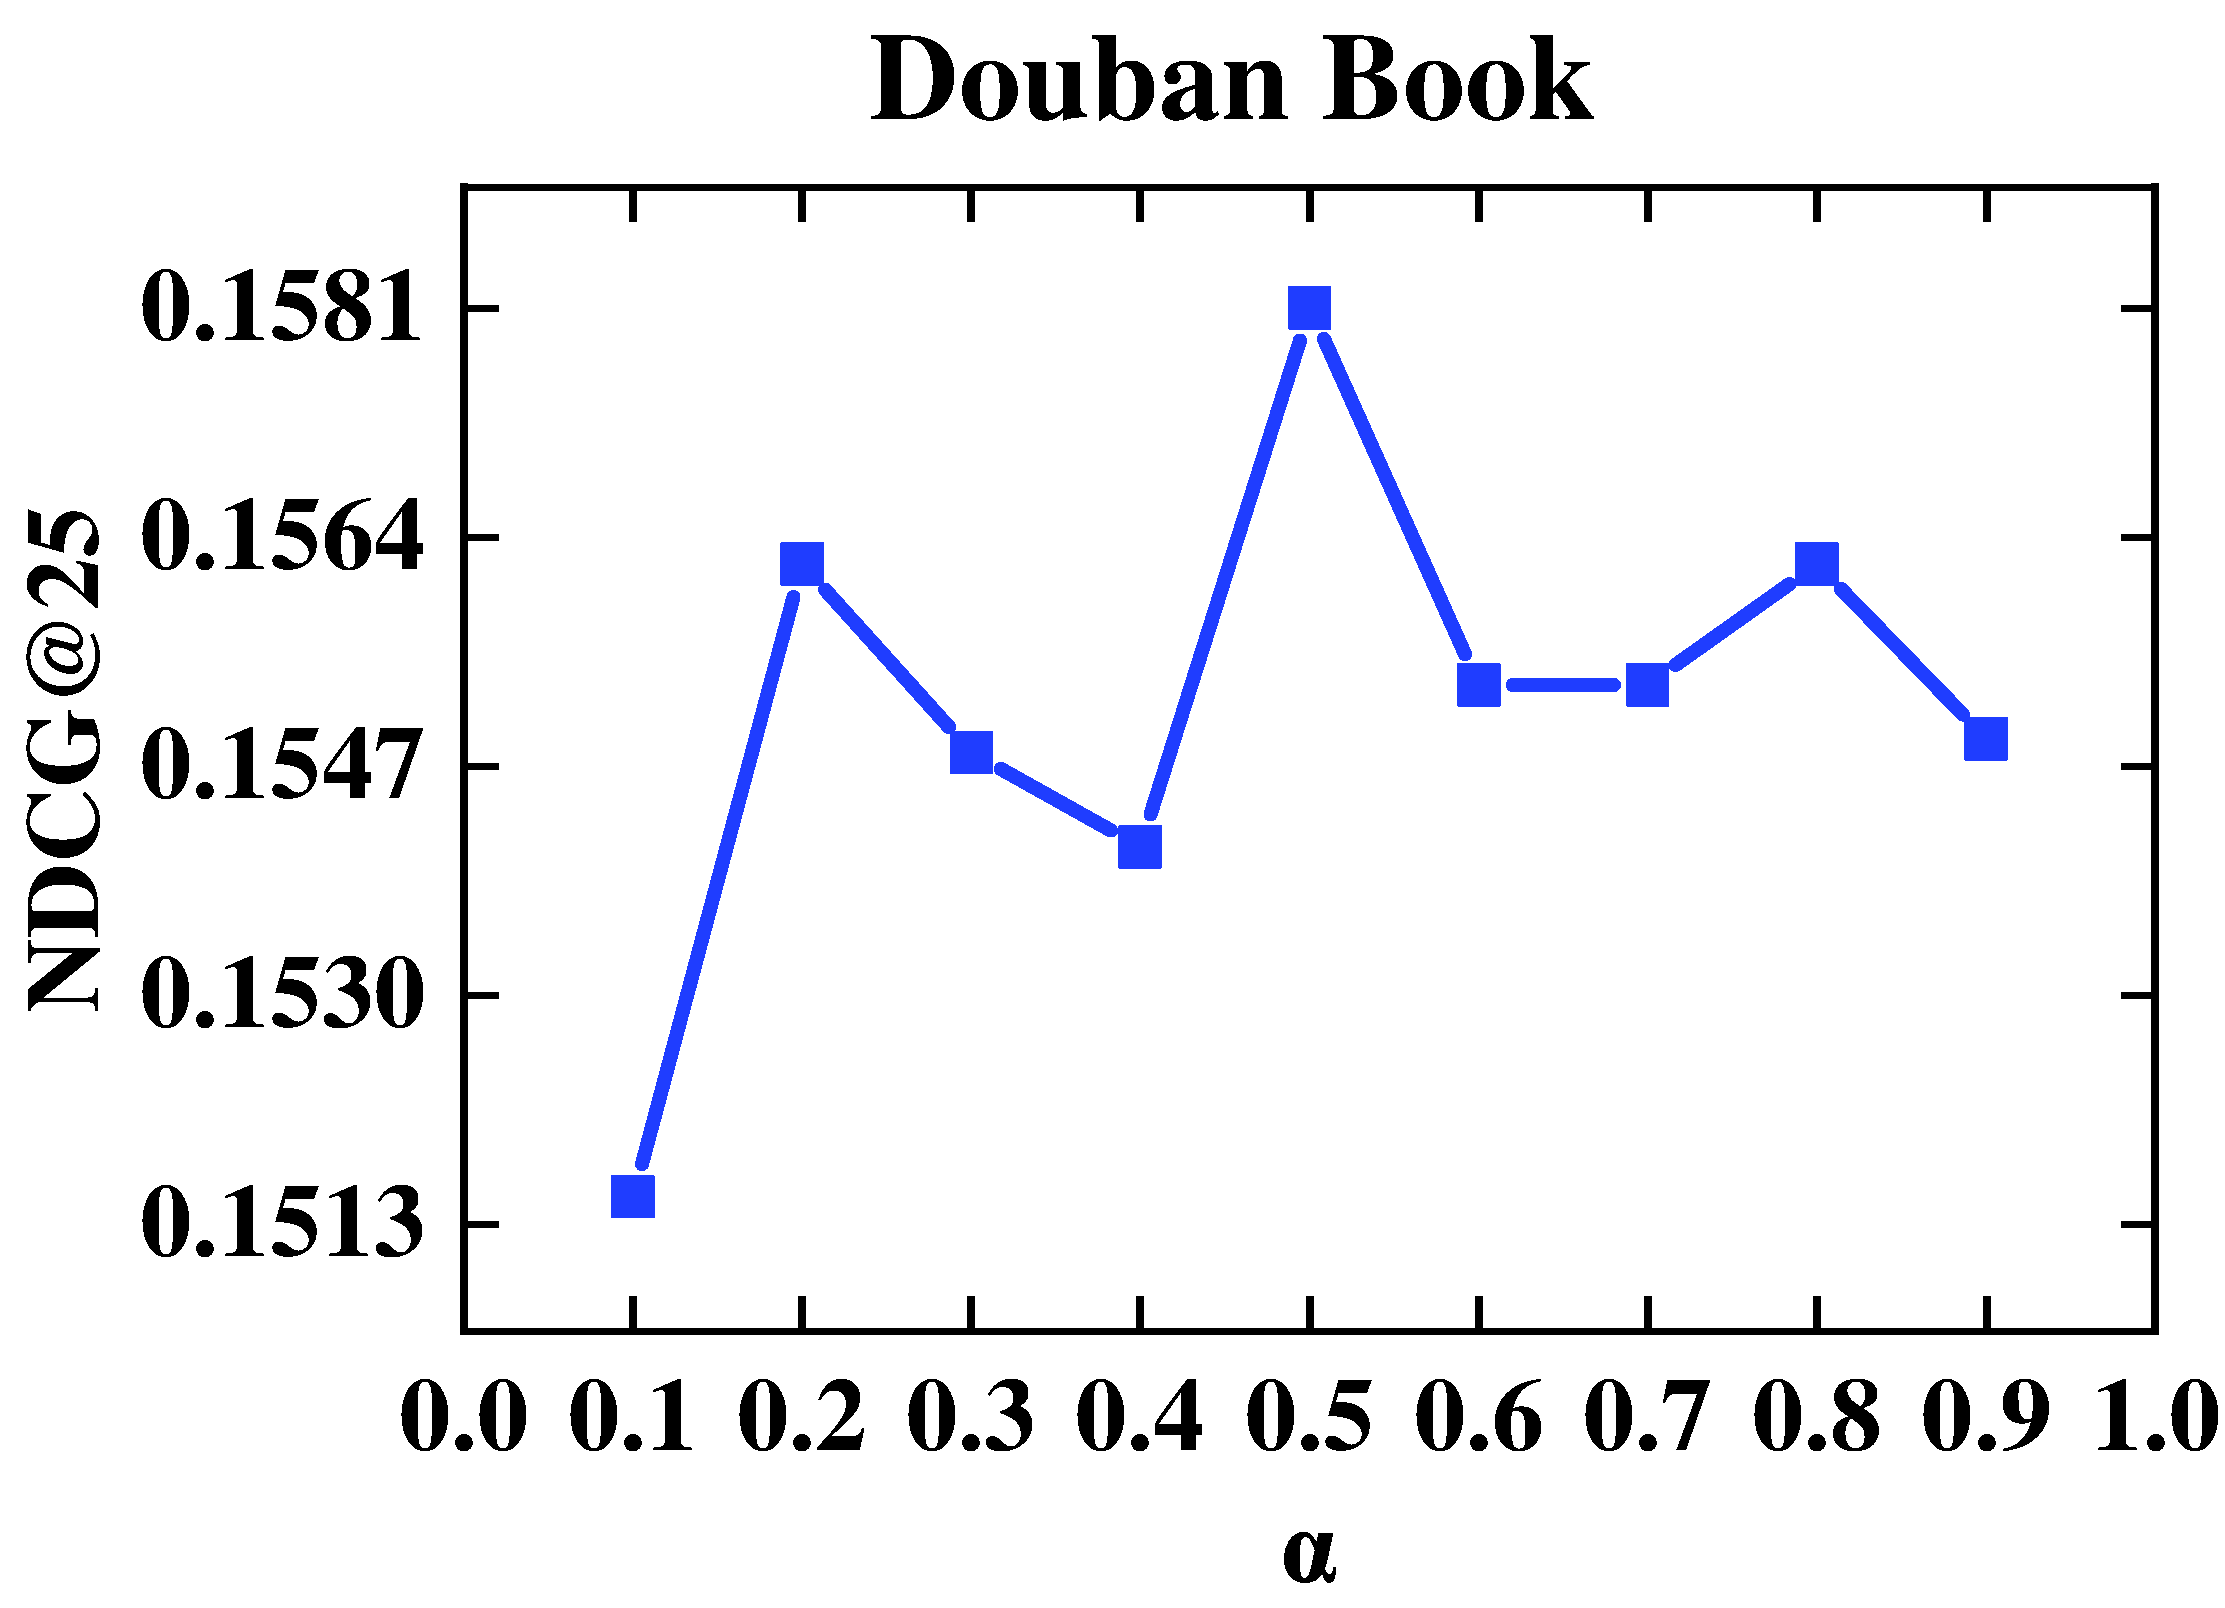
\includegraphics[width=0.4\textwidth]{fig/par/9.pdf}
    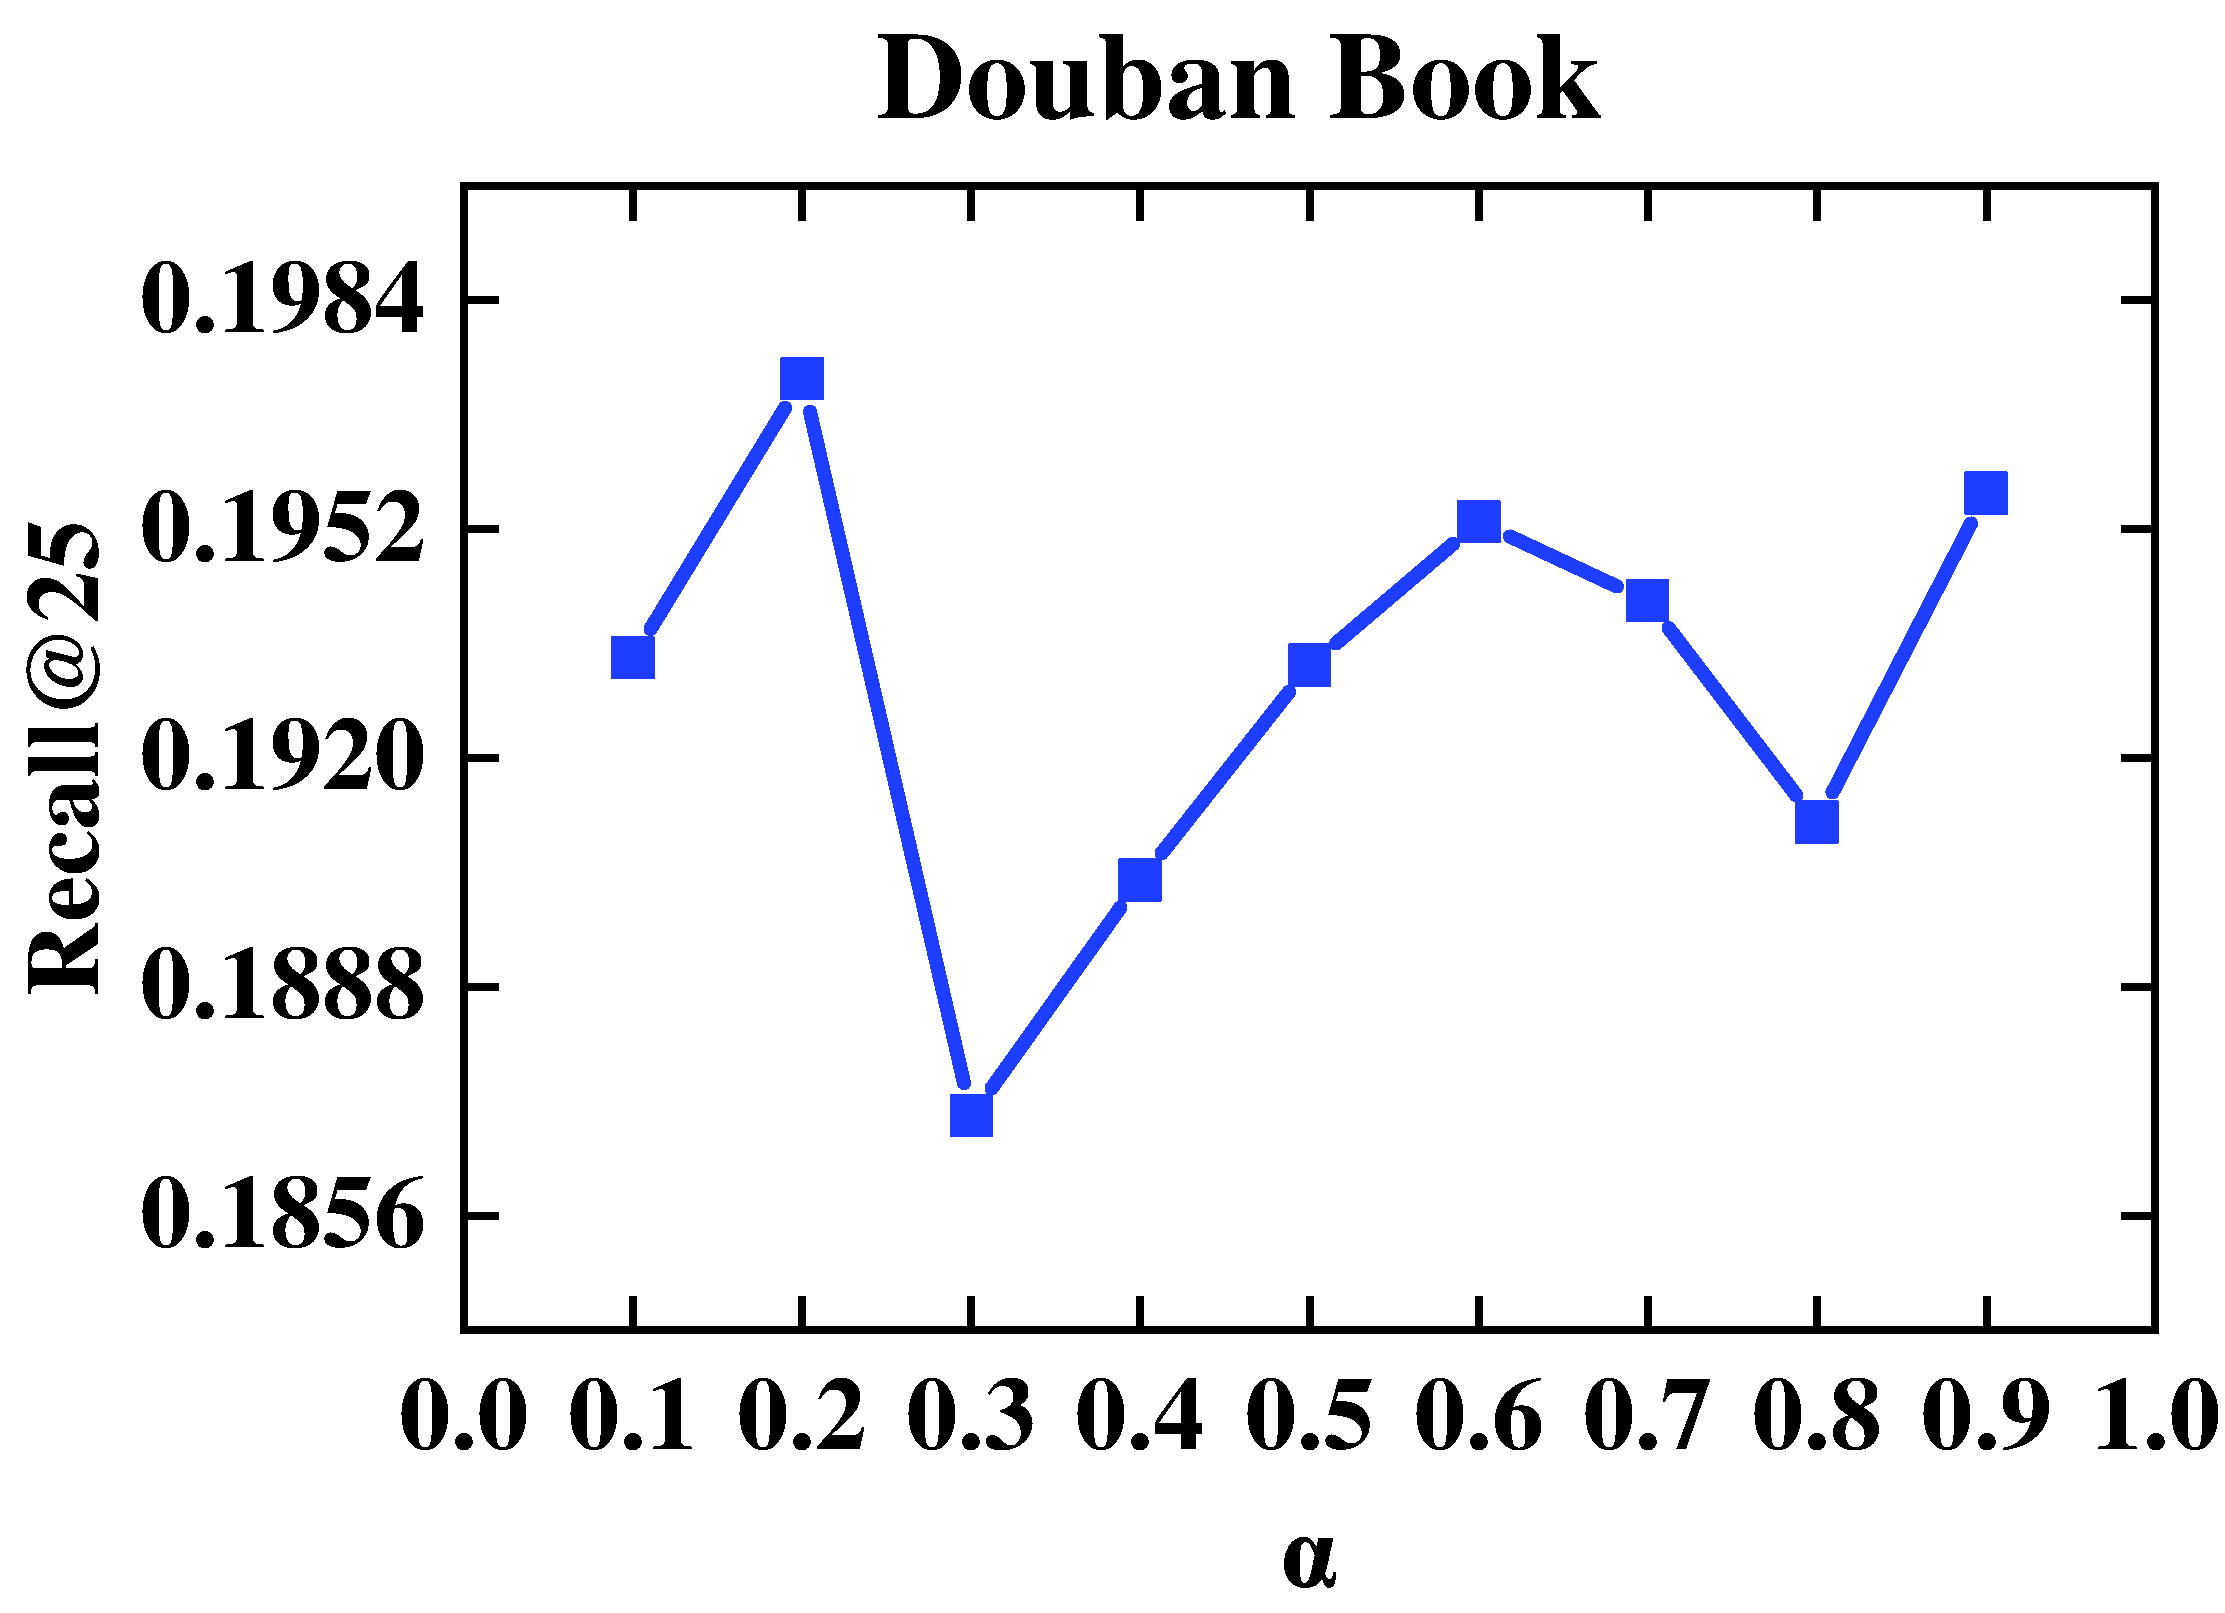
\includegraphics[width=0.4\textwidth]{fig/par/10.pdf}
    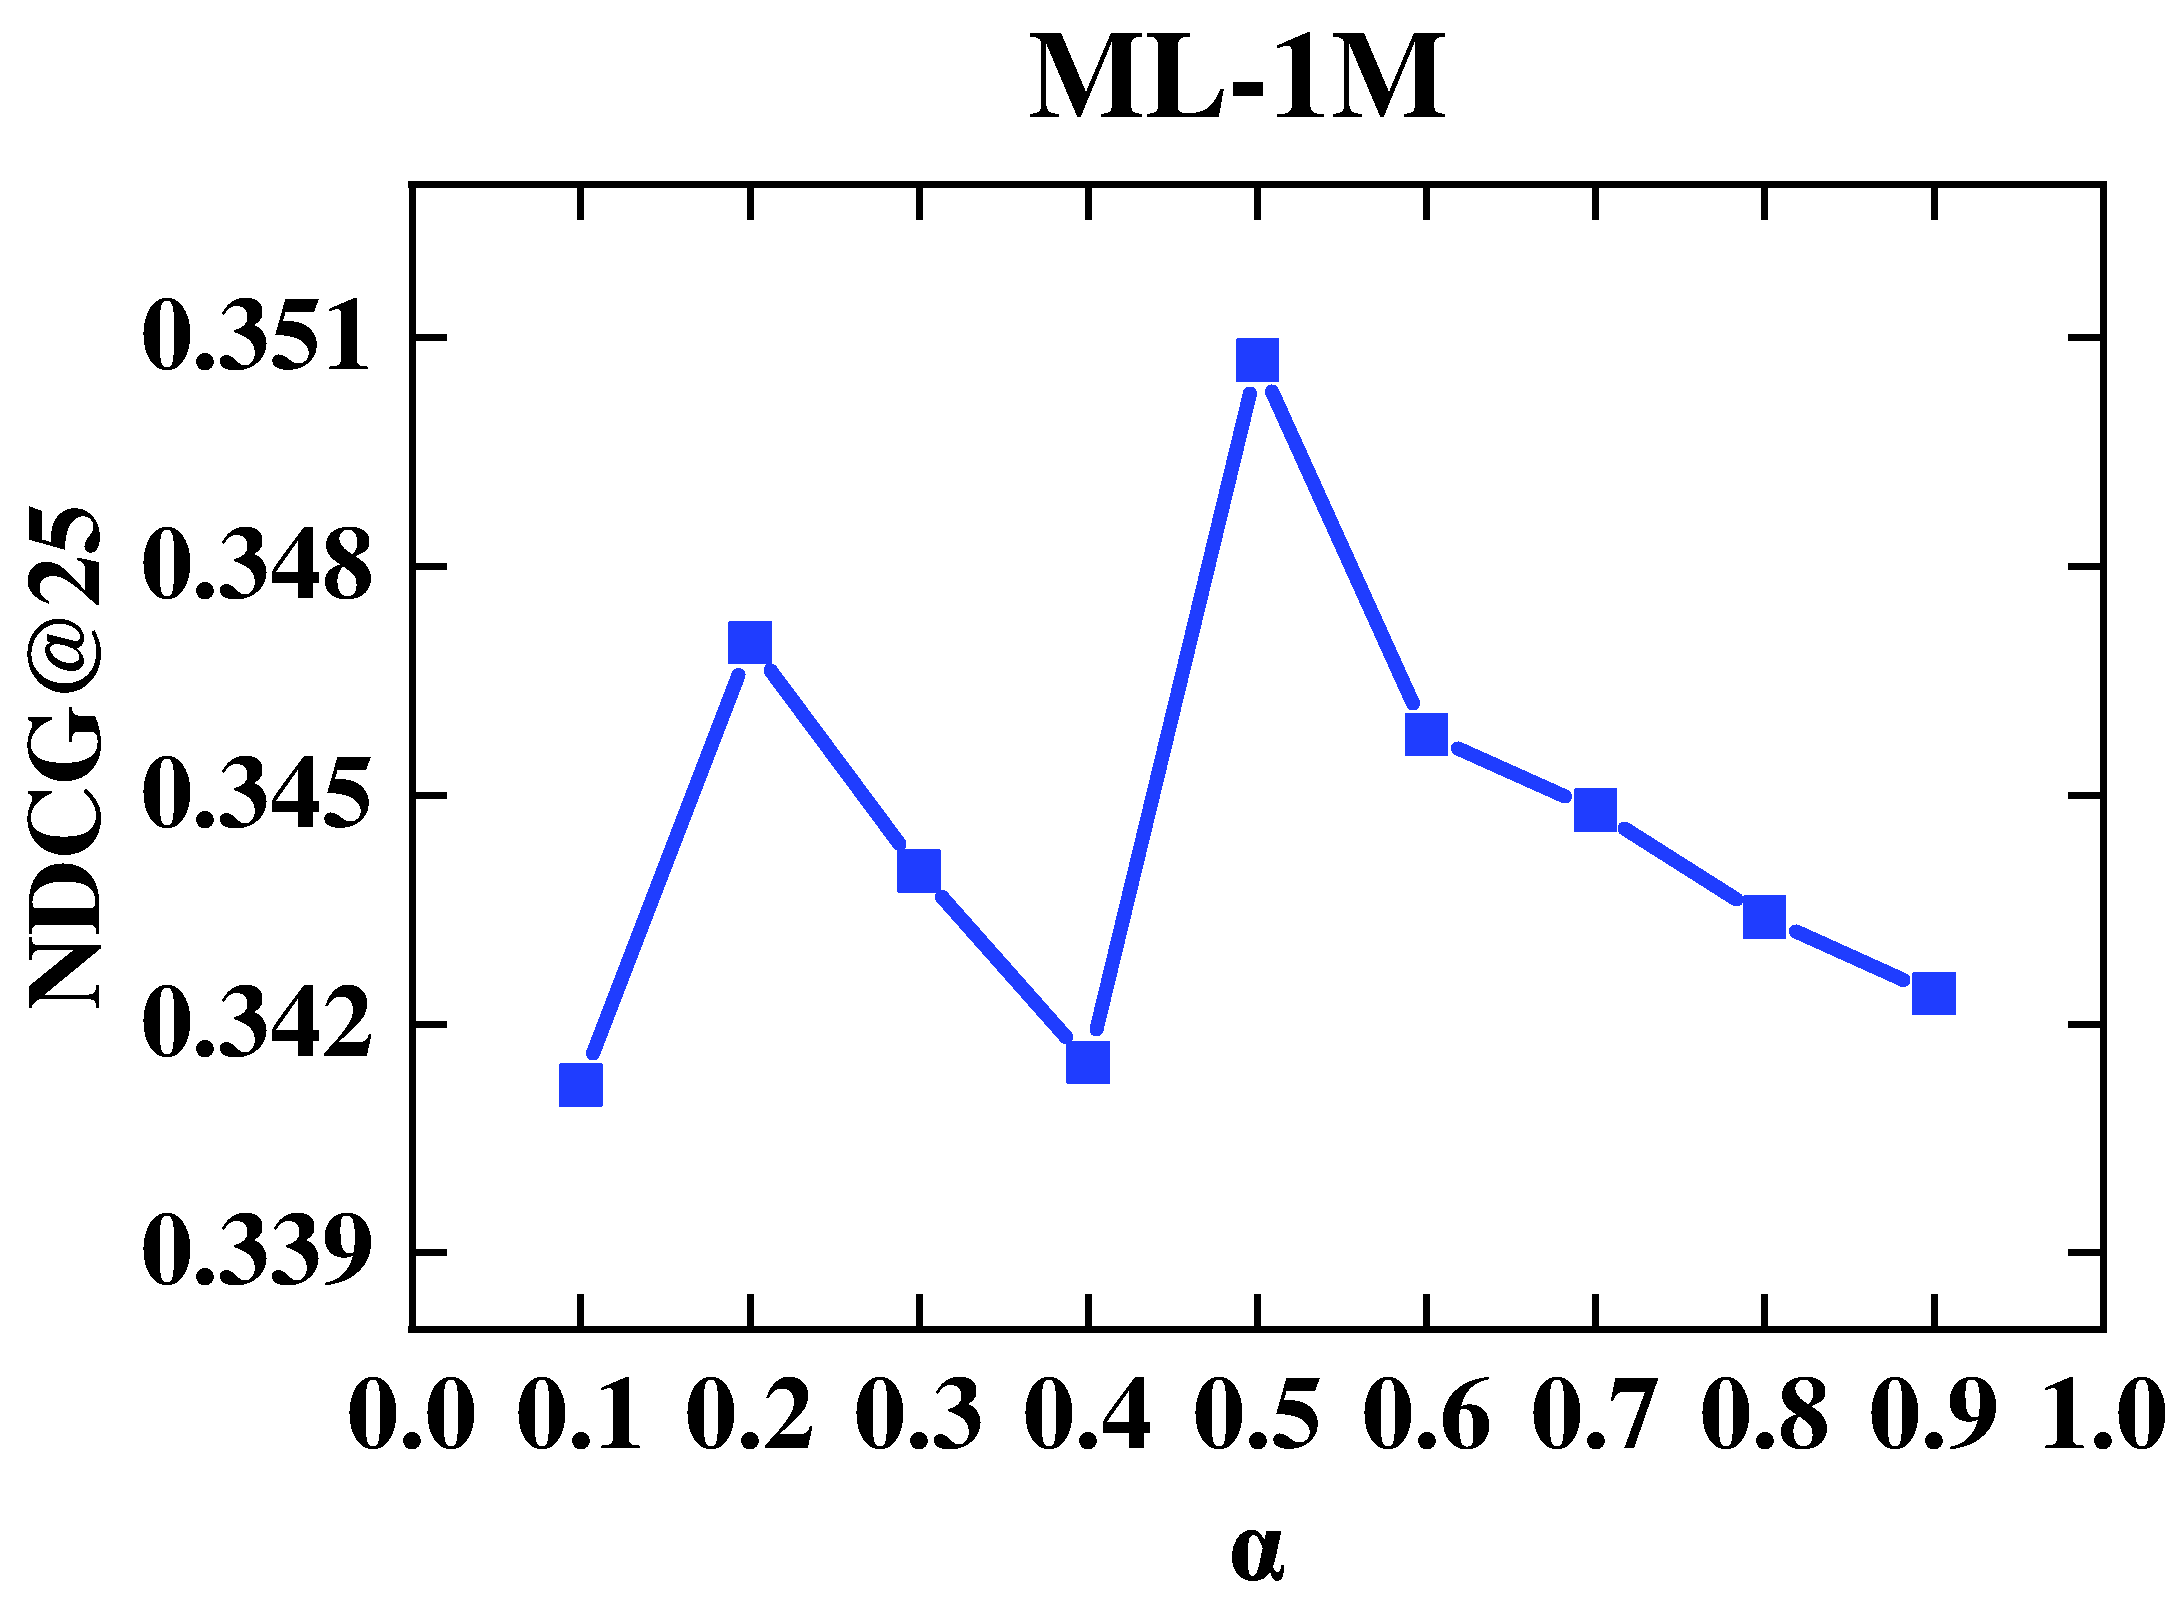
\includegraphics[width=0.4\textwidth]{fig/par/11.pdf}
    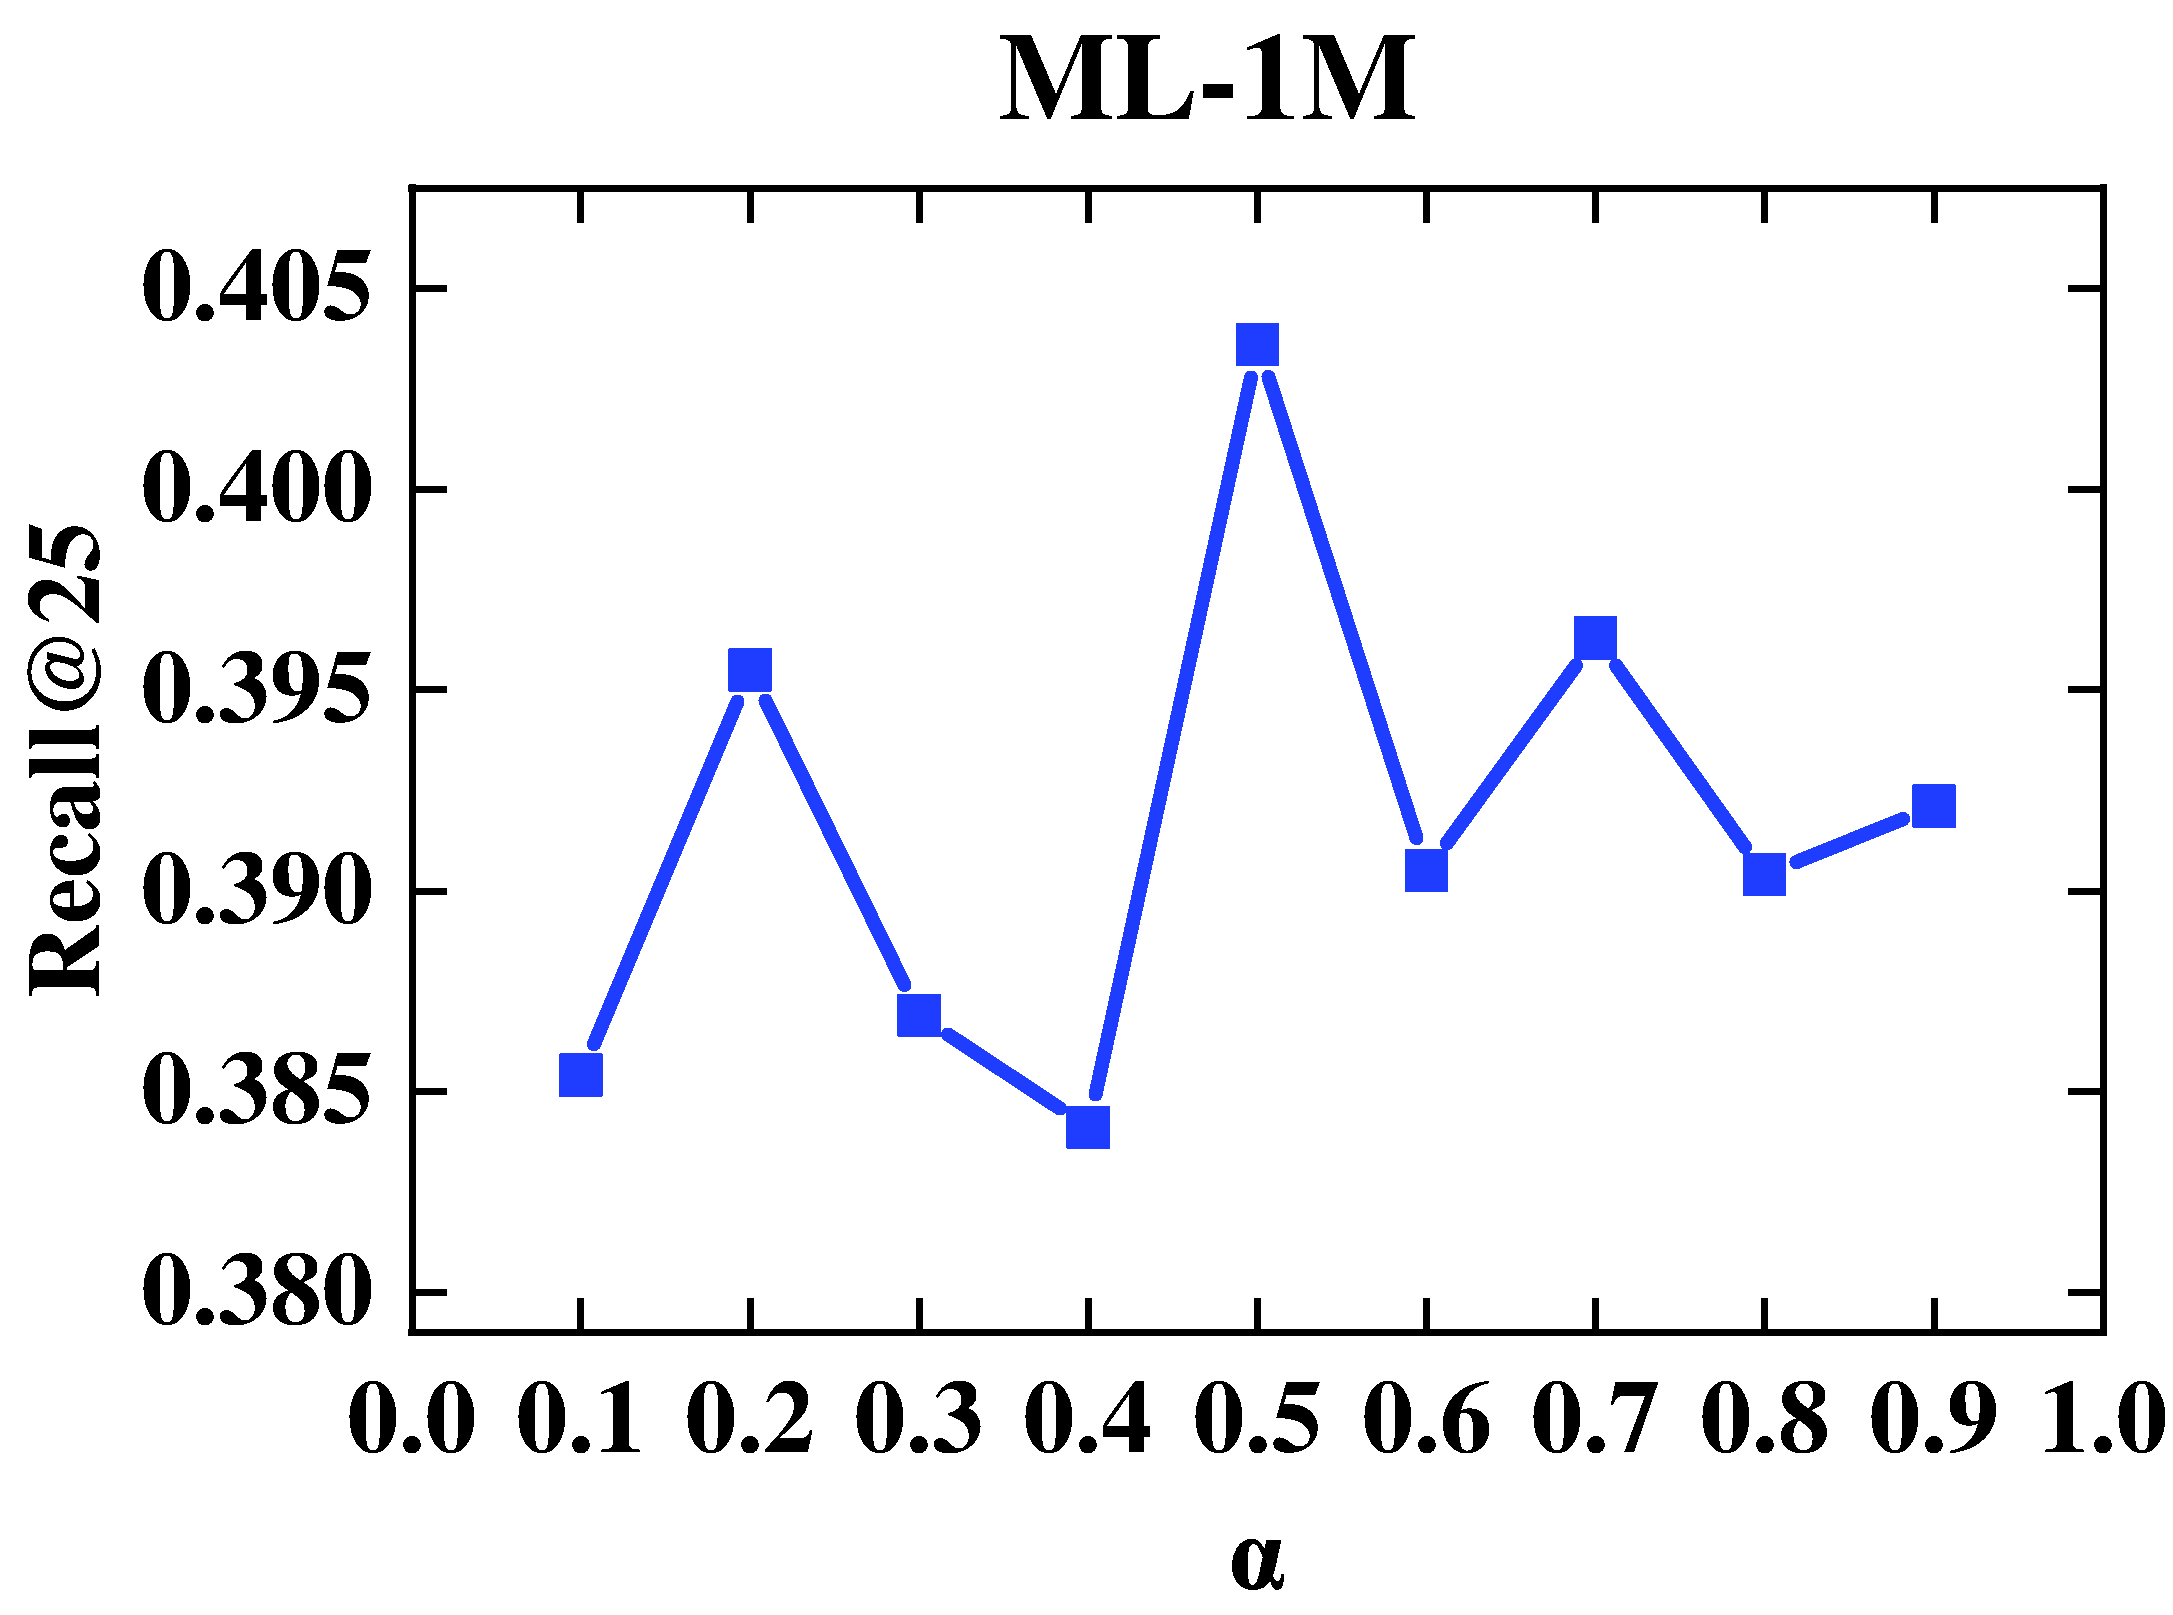
\includegraphics[width=0.4\textwidth]{fig/par/12.pdf}}

\caption{Impact of $\alpha$ on ML-1M, Douban Book } \label{alpha}
\end{figure*}

\subsubsection{Effect of SSL weight $\alpha$}\label{subsubsec2}

In this part, we discuss the effect of dropout ratio $\alpha$. The results are presented in Fig. \ref{alpha} in terms of NDCG@25 and Recall@25 on ML-1M and Douban Book datasets. As shown in Fig. \ref{alpha}, the best performance of ML-1M is obtained when $\alpha$ is 0.5 and best performance of Douban Book is obtained when $\alpha$ at around 0.5. We can observe that the performance curves of DSVAE trend to be worse when $\alpha$ exceeds a threshold.  It is not hard to explain that, when the value of $\alpha$ is too small, the interaction has a lower possibility to be contained in augmented data so that SSL task contributes less or even damages the performance of the main task.

\subsubsection{Effect of negative samples $\mathbf{N}_i$} \label{subsubsec2}
$\mathbf{N}_i$ controls sampling space of $\mathcal{L}_{rcl}$ on each user. We varied the amount of negative samples and summarized the performance in Fig. \ref{N_u}. 

We find that best result is achieved with different value of $\mathbf{N}_i$ for two datasets, where a large $\mathbf{N}_i$ leads to a better performance in most cases. On the other hand, large $\mathbf{N}_i$ will draw more noise into the learning framework and small $\mathbf{N}_i$ will lose more valuable information, two of which have negative effects on the learning model.




\begin{figure*}[!htb]
\centering

{\label{lambda}
    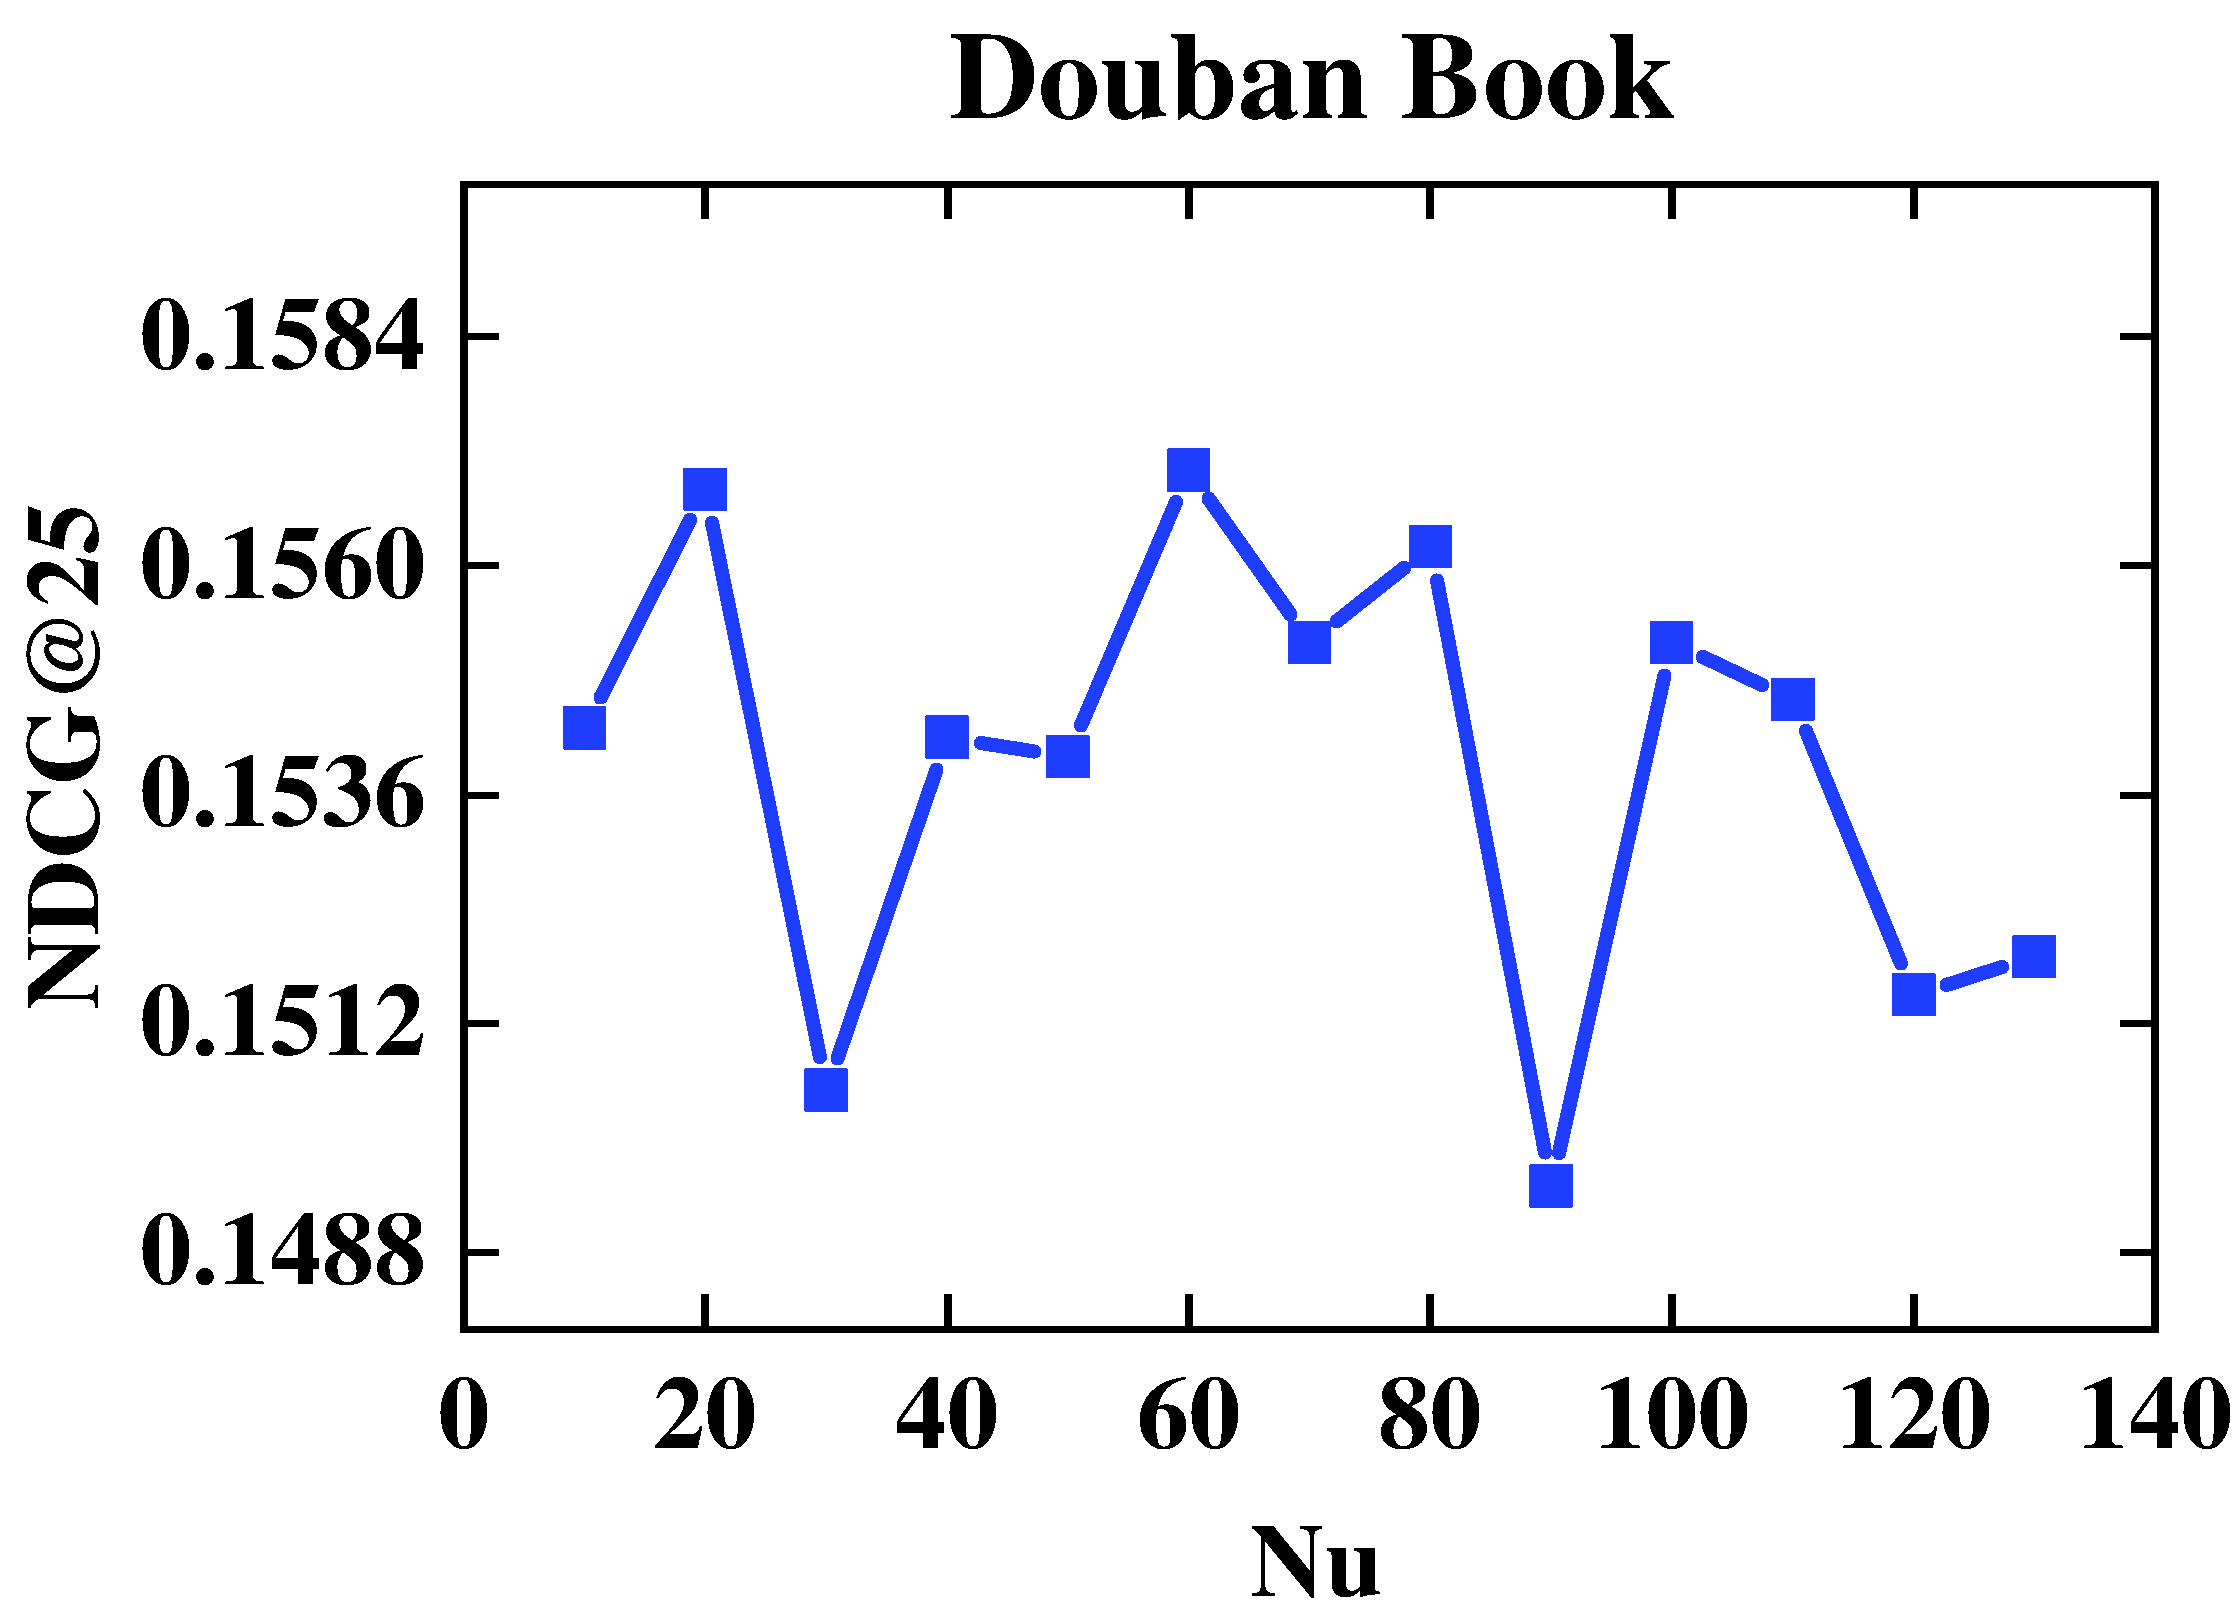
\includegraphics[width=0.4\textwidth]{fig/par/13.pdf}
    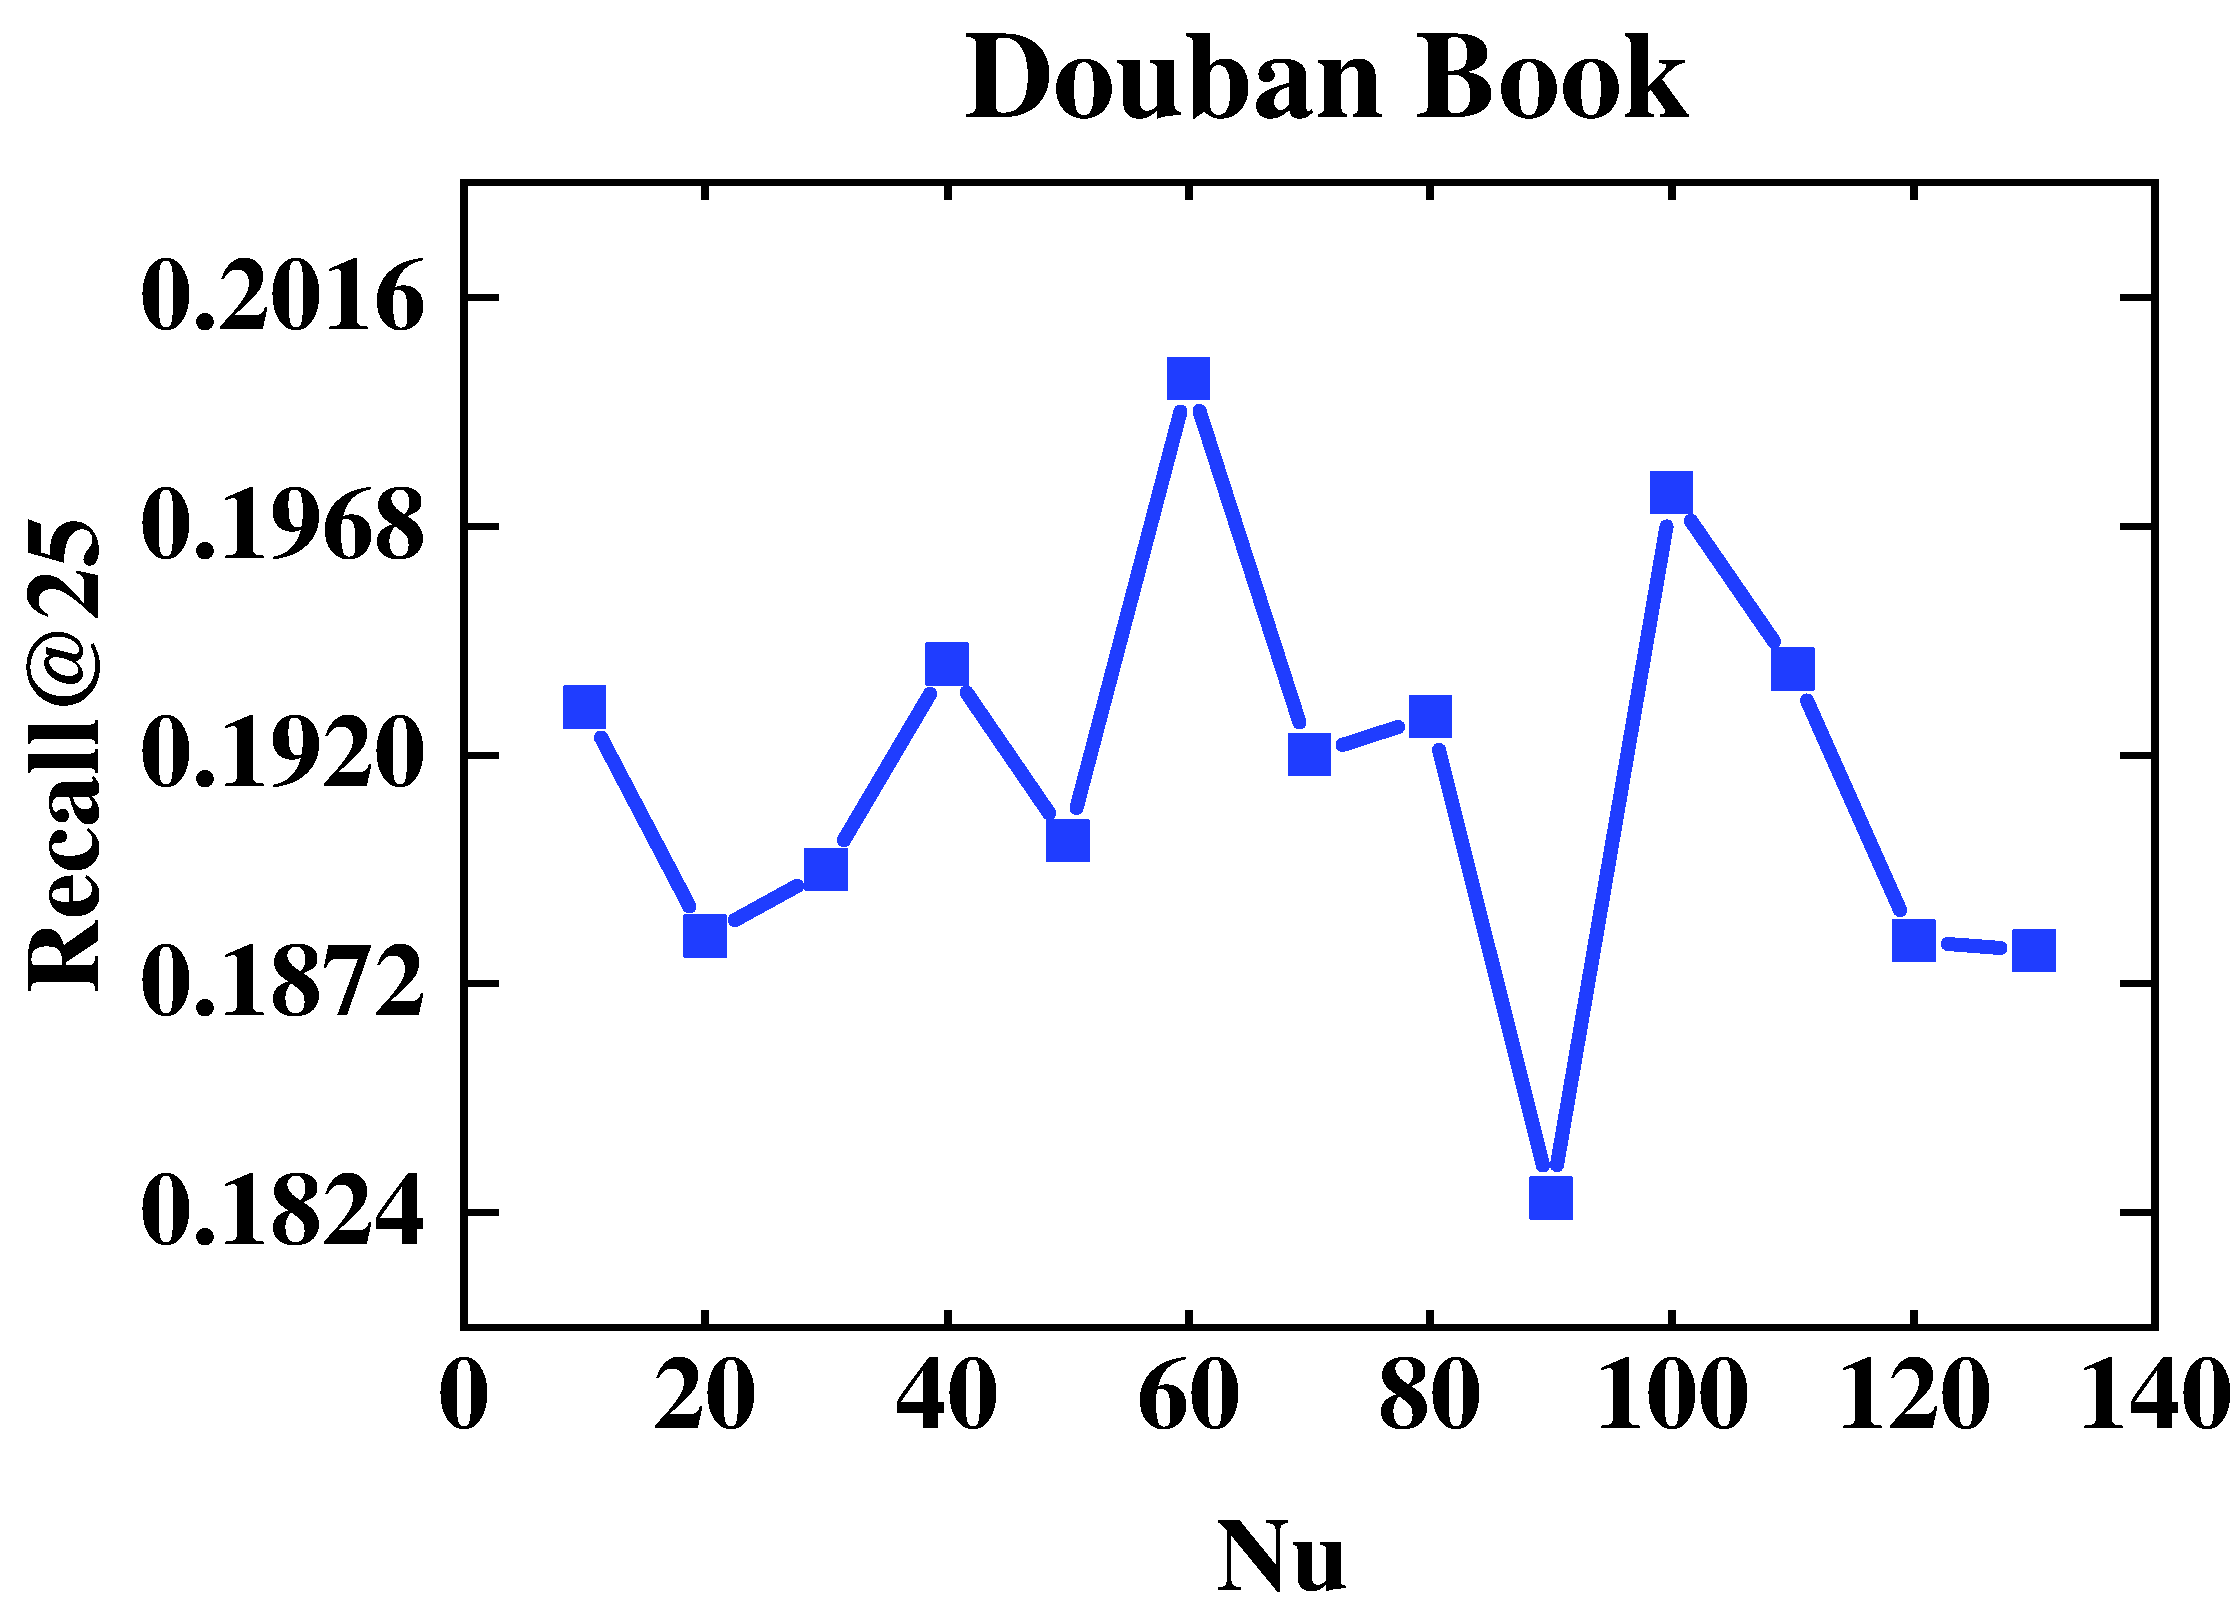
\includegraphics[width=0.4\textwidth]{fig/par/14.pdf}
    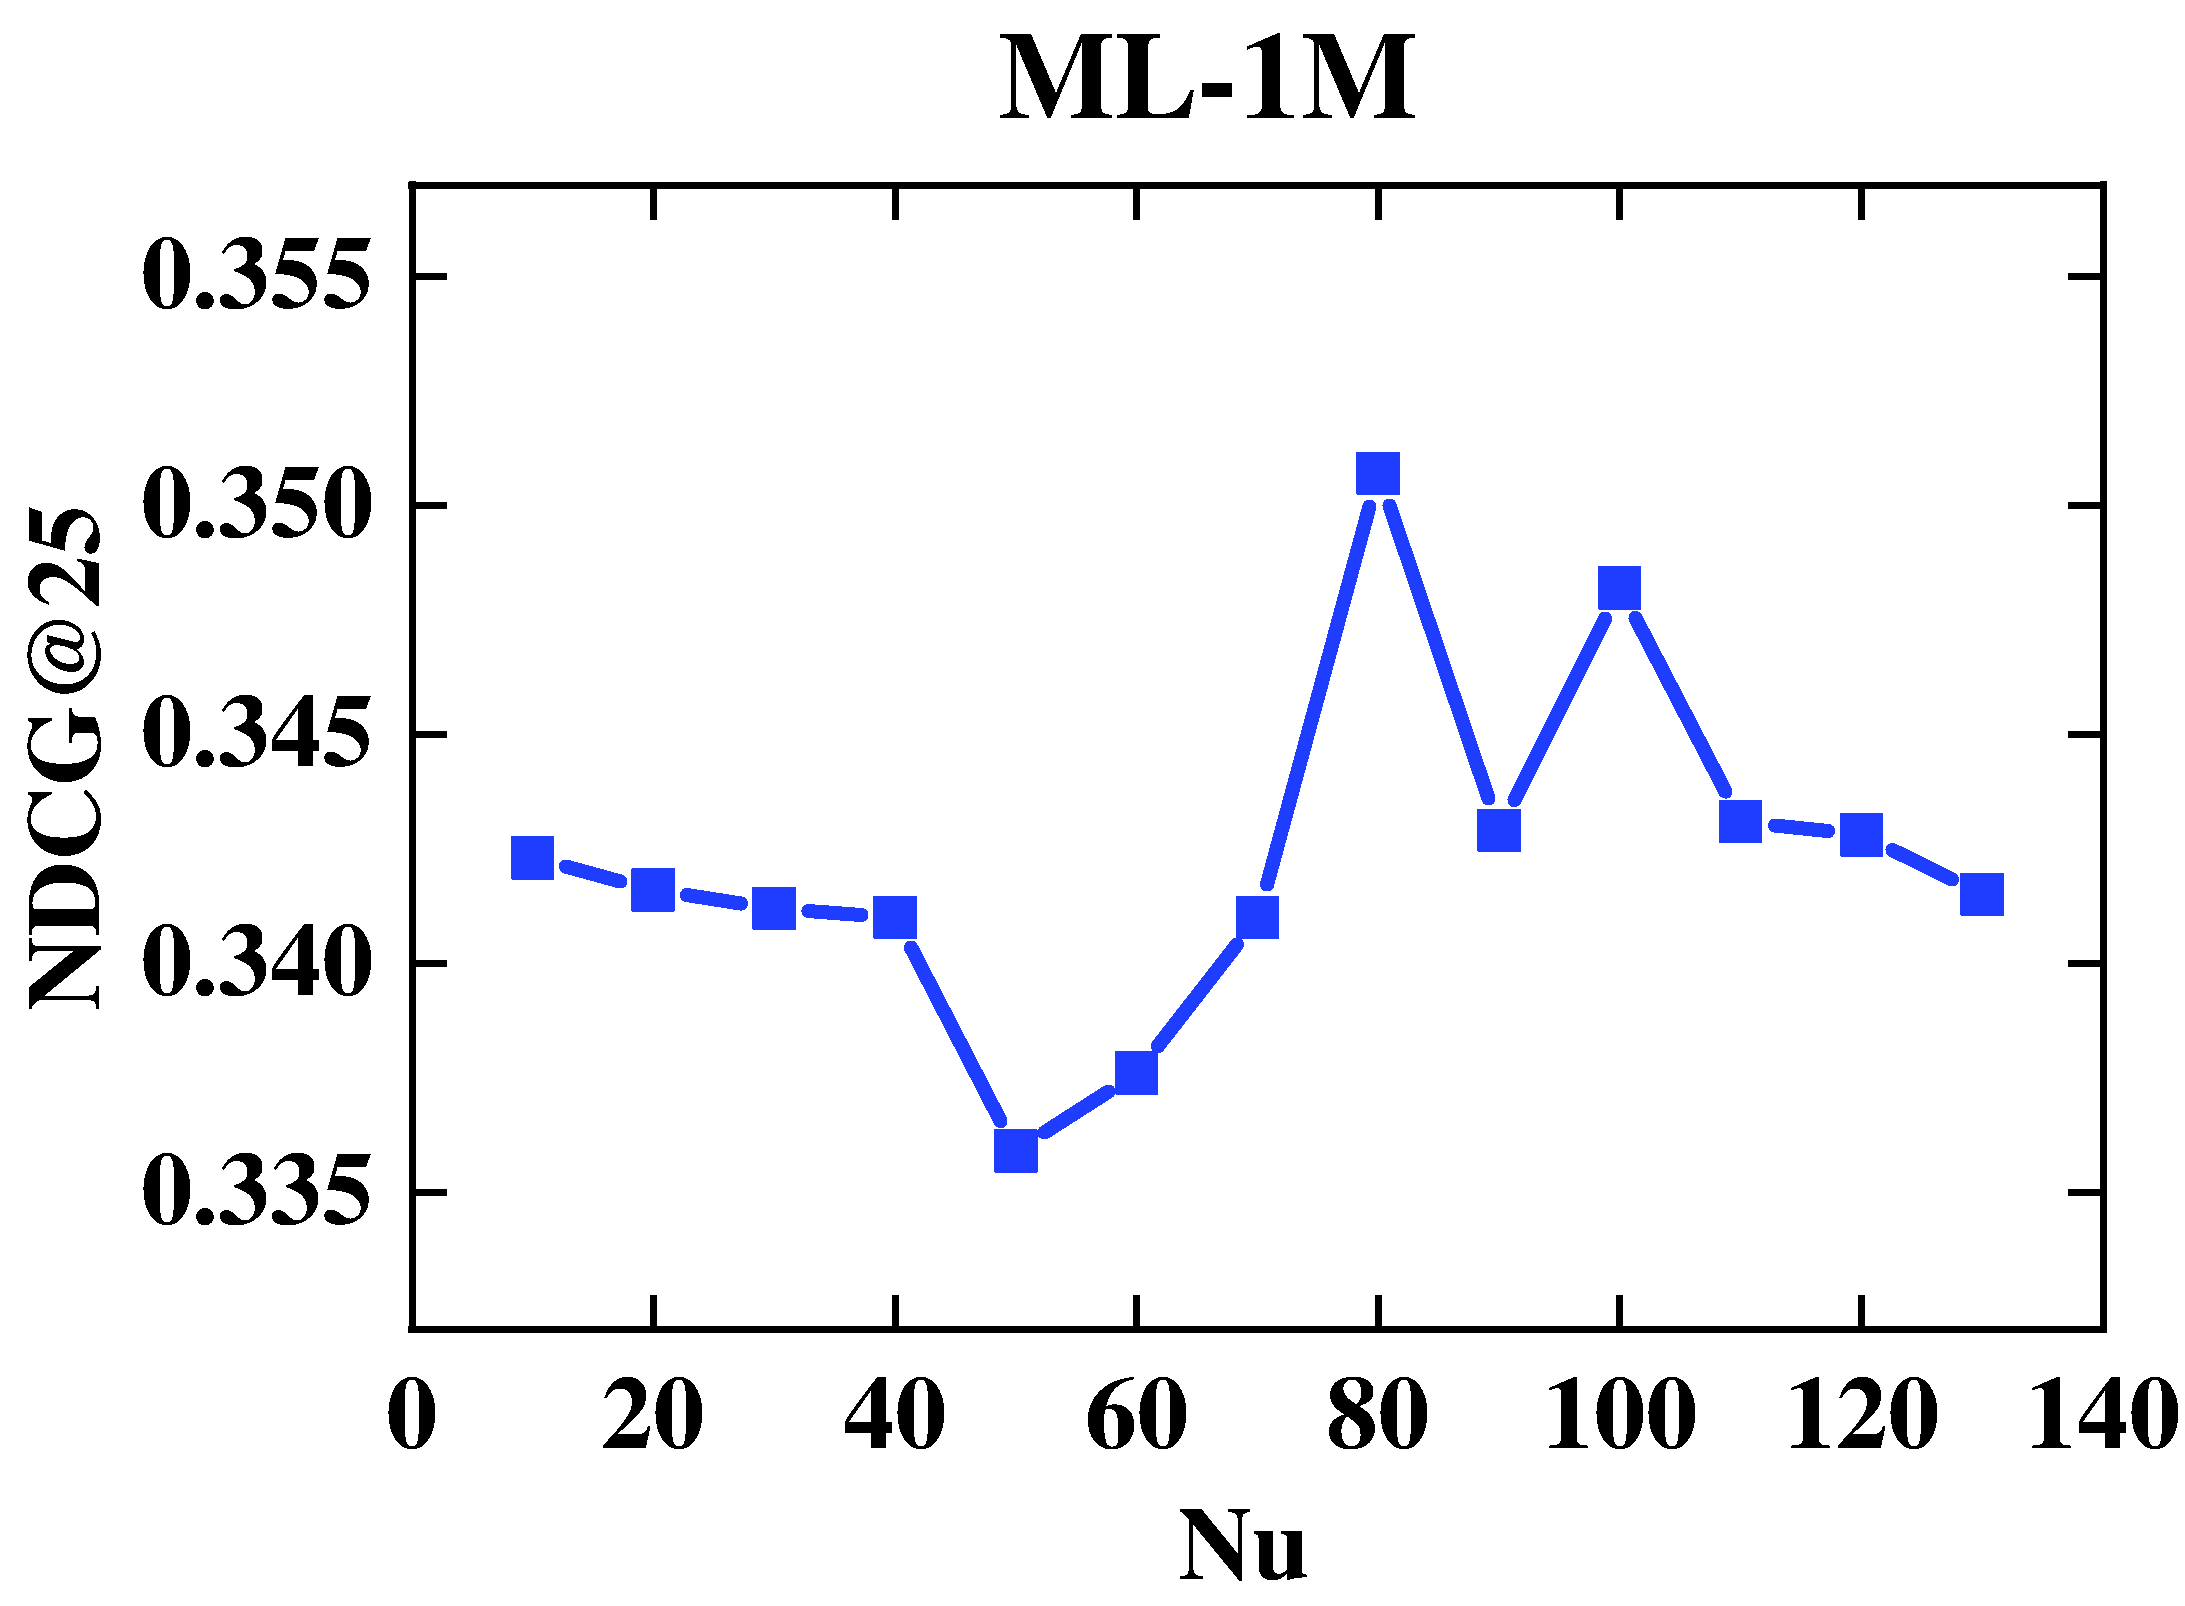
\includegraphics[width=0.4\textwidth]{fig/par/15.pdf}
    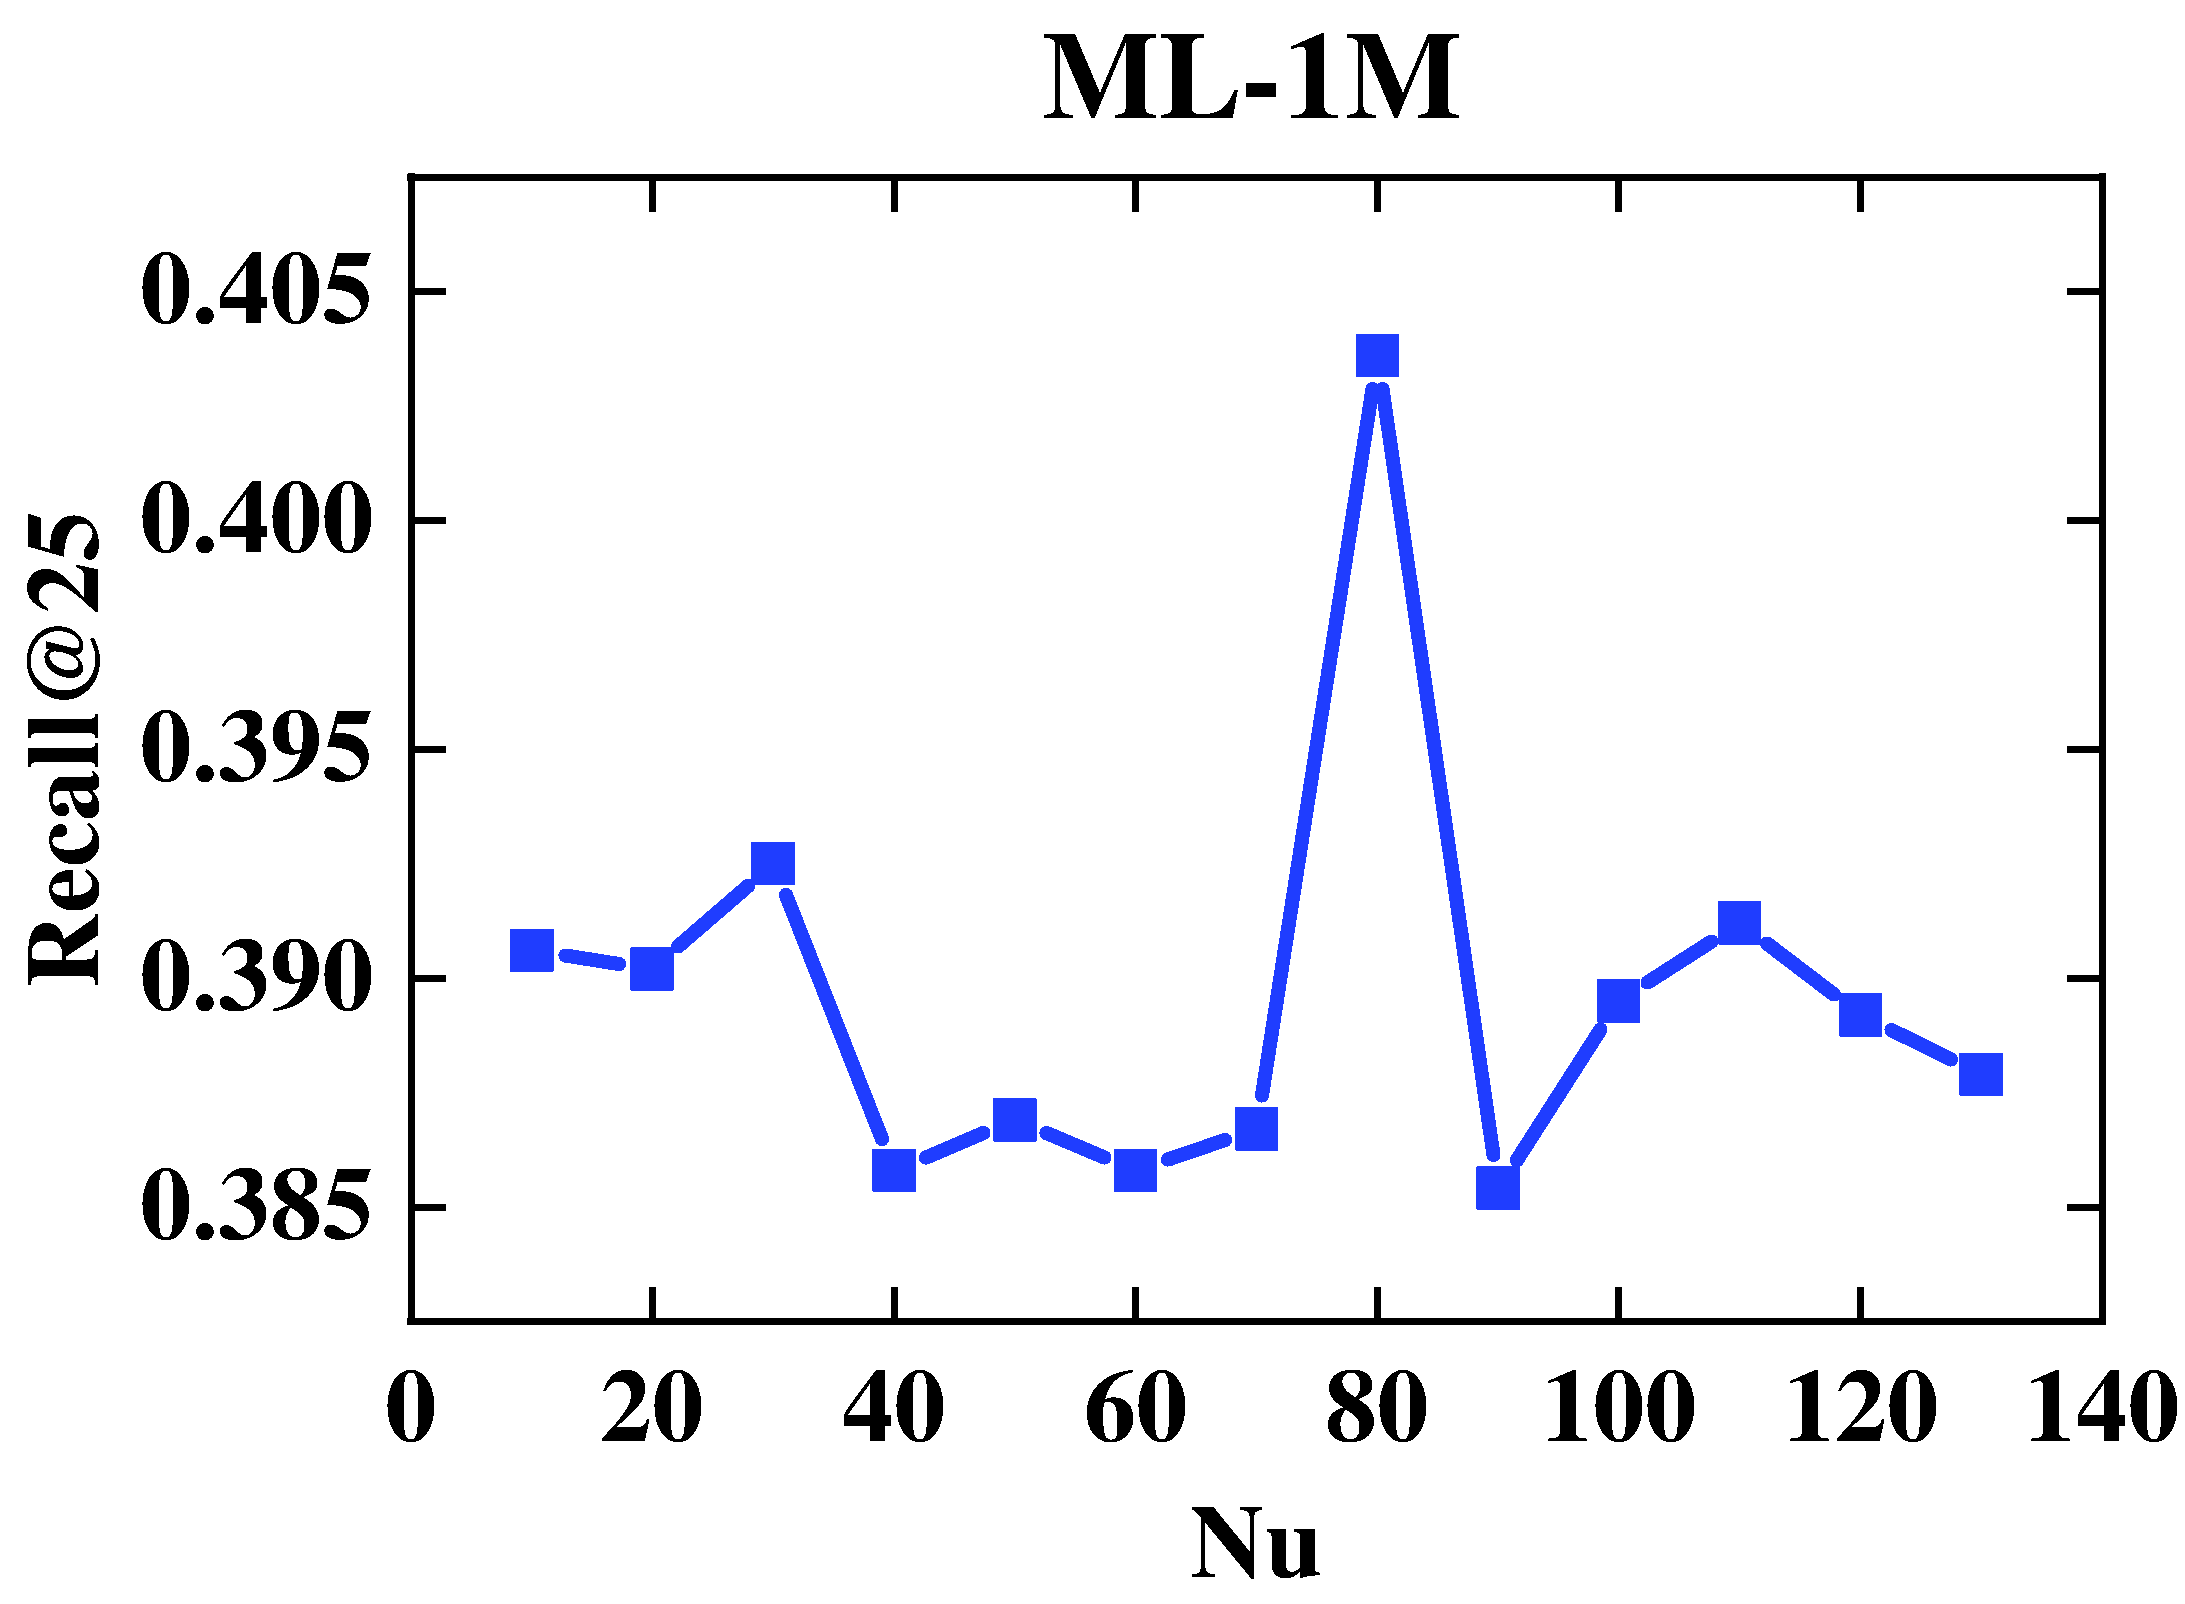
\includegraphics[width=0.4\textwidth]{fig/par/16.pdf}}
\caption{Impact of $\mathbf{N}_i$ on ML-1M, Douban Book } \label{N_u}
\end{figure*}



\section{Conclusion}\label{sec5}
In this paper, we have developed DSVAE, a new framework that integrates  two self-supervised tasks into a single variational autoencoder framework. In sharp contrast to existing VAE based CF models, our DSVAE approach considers both intrinsical correlation and individual difference to improve both the generalization ability of VAE model on sparse interaction datasets  and  personalized characteristic of recommendation results. Extensive experiments demonstrated that our DSVAE approach achieves better performance than state-of-the-art methods. In the future, we will create more powerful self-supervised tasks, as well as research on a per-train model which  utilizes self-supervised learning to obtain general user representation and then fine-tune top-K recommendation task with supervision signals.








%\begin{acknowledgements}
%If you'd like to thank anyone, place your comments here
%and remove the percent signs.
%\end{acknowledgements}


% Authors must disclose all relationships or interests that 
% could have direct or potential influence or impart bias on 
% the work: 
%
% \section*{Conflict of interest}
%
% The authors declare that they have no conflict of interest.

%\bibliographystyle{IEEEtran}
\bibliographystyle{spbasic}
\bibliography{reference}
% BibTeX users please use one of
%\bibliographystyle{spbasic}      % basic style, author-year citations
%\bibliographystyle{spmpsci}      % mathematics and physical sciences
%\bibliographystyle{spphys}       % APS-like style for physics
%\bibliography{}   % name your BibTeX data base

% Non-BibTeX users please use
%\begin{thebibliography}{}
%
% and use \bibitem to create references. Consult the Instructions
% for authors for reference list style.
%
%\bibitem{RefJ}
% Format for Journal Reference
%Author, Article title, Journal, Volume, page numbers (year)
% Format for books
%\bibitem{RefB}
%Author, Book title, page numbers. Publisher, place (year)
% etc
%\end{thebibliography}

\end{document}
% end of file template.tex

